%\documentclass[gmd,hvmath,online]{copernicus_discussions}  % to submit use this style
%DIF LATEXDIFF DIFFERENCE FILE
%DIF DEL draft-gmd-hydro.tex   Sun Feb  8 15:26:05 2015
%DIF ADD gmd-hydro.tex         Sun Feb  8 15:26:13 2015
\documentclass[gmd]{copernicus}   % two-column layout

\usepackage{amssymb,xspace}
\usepackage[T1]{fontenc}

% hyperref should be the last package we load
%DIF 8c8
%DIF < \usepackage[draft,pdftex,
%DIF -------
\usepackage[pdftex, %DIF > 
%DIF -------
                colorlinks=true,
                plainpages=false, % only if colorlinks=true
                linkcolor=blue,   % only if colorlinks=true
                citecolor=black,   % only if colorlinks=true
                urlcolor=magenta     % only if colorlinks=true
]{hyperref}

\ifx\text\undefined
\newcommand{\text}{\textrm}
\else
\fi

% math macros
\newcommand\bv{\mathbf{v}}
\newcommand\bV{\mathbf{V}}
\newcommand\bq{\mathbf{q}}
\newcommand\bQ{\mathbf{Q}}

\newcommand{\ddt}[1]{\ensuremath{\frac{\partial #1}{\partial t}}}
\newcommand{\Div}{\nabla\cdot}
\newcommand\eps{\epsilon}
\newcommand{\grad}{\nabla}

\newcommand{\Ntil}{N_{\text{til}}}
\newcommand{\hatNtil}{\hat N_{\text{til}}}
\newcommand{\Wtil}{W_{\text{til}}}
\newcommand{\Wtilmax}{W_{\text{til}}^{\text{max}}}

\newcommand{\Wlij}{W^l_{i,j}}
\newcommand{\Wij}{W_{i,j}}
\newcommand{\Plij}{P^l_{i,j}}
\newcommand{\Pij}{P_{i,j}}

\newcommand{\Nbreen}{Nordenski\"oldbreen\xspace}
 %DIF > 
\usepackage[]{lineno} %DIF > 
%DIF PREAMBLE EXTENSION ADDED BY LATEXDIFF
%DIF UNDERLINE PREAMBLE %DIF PREAMBLE
\RequirePackage[normalem]{ulem} %DIF PREAMBLE
\RequirePackage{color}\definecolor{RED}{rgb}{1,0,0}\definecolor{BLUE}{rgb}{0,0,1} %DIF PREAMBLE
\providecommand{\DIFadd}[1]{{\protect\color{blue}\uwave{#1}}} %DIF PREAMBLE
\providecommand{\DIFdel}[1]{{\protect\color{red}\sout{#1}}}                      %DIF PREAMBLE
%DIF SAFE PREAMBLE %DIF PREAMBLE
\providecommand{\DIFaddbegin}{} %DIF PREAMBLE
\providecommand{\DIFaddend}{} %DIF PREAMBLE
\providecommand{\DIFdelbegin}{} %DIF PREAMBLE
\providecommand{\DIFdelend}{} %DIF PREAMBLE
%DIF FLOATSAFE PREAMBLE %DIF PREAMBLE
\providecommand{\DIFaddFL}[1]{\DIFadd{#1}} %DIF PREAMBLE
\providecommand{\DIFdelFL}[1]{\DIFdel{#1}} %DIF PREAMBLE
\providecommand{\DIFaddbeginFL}{} %DIF PREAMBLE
\providecommand{\DIFaddendFL}{} %DIF PREAMBLE
\providecommand{\DIFdelbeginFL}{} %DIF PREAMBLE
\providecommand{\DIFdelendFL}{} %DIF PREAMBLE
%DIF END PREAMBLE EXTENSION ADDED BY LATEXDIFF

\begin{document}
\graphicspath{{figszip/}}

%\linenumbers

\title{Mass-conserving subglacial hydrology in \DIFdelbegin %DIFDELCMD < \\ %%%
\DIFdelend the Parallel Ice Sheet Model \DIFaddbegin \DIFadd{version 0.6}\DIFaddend }


\author[1]{E.~Bueler}
\author[2]{W.~\DIFdelbegin \DIFdel{Van }\DIFdelend \DIFaddbegin {\DIFadd{van}} \DIFaddend Pelt}

\affil[1]{Department of Mathematics and Statistics, University of Alaska Fairbanks, Alaska, USA}
\affil[2]{Institute for Marine and Atmospheric Research Utrecht, The Netherlands\footnote{Current address: Norwegian Polar Institute, Tromsø, Norway}}

%% The [] brackets identify the author to the corresponding affiliation, 1, 2, 3, etc. should be inserted.

\runningtitle{Subglacial hydrology in PISM}
\DIFdelbegin %DIFDELCMD < \runningauthor{Bueler and Van Pelt}
%DIFDELCMD < %%%
\DIFdelend \DIFaddbegin \runningauthor{Bueler and {van} Pelt}
\DIFaddend 

\correspondence{Ed Bueler (\texttt{elbueler@alaska.edu})}

%% These dates will be inserted by the Publication Production Office during the typesetting process.
\received{}
\pubdiscuss{} %% only important for two-stage journals
\revised{}
\accepted{}
\published{}

\firstpage{1}

\maketitle

\begin{abstract}
We describe and test a \DIFdelbegin \DIFdel{distributed }\DIFdelend \DIFaddbegin \DIFadd{two-horizontal-dimension }\DIFaddend subglacial hydrology model which combines \DIFdelbegin \DIFdel{a pressurized, plastic }\DIFdelend till with a \DIFaddbegin \DIFadd{distributed }\DIFaddend system of water-filled, linked cavities which open through \DIFdelbegin \DIFdel{sliding-generated cavitation  }\DIFdelend \DIFaddbegin \DIFadd{sliding }\DIFaddend and close through ice creep.  The addition of this sub-model to the Parallel Ice Sheet Model accomplishes three specific goals: (1) conservation of the mass of \DIFdelbegin \DIFdel{two-phase (solid/liquid) waterin the ice sheet}\DIFdelend \DIFaddbegin \DIFadd{water}\DIFaddend , (2) simulation of spatially- and temporally-variable basal shear stress from physical mechanisms based on a minimal number of free parameters, and (3) convergence under \DIFdelbegin \DIFdel{two-horizontal-dimensional grid refinementof the subglacial water amount and pressure}\DIFdelend \DIFaddbegin \DIFadd{grid refinement}\DIFaddend .  The model is a common generalization of \DIFdelbegin \DIFdel{at least }\DIFdelend four others: (i) the undrained plastic bed model of \cite{Tulaczyketal2000b}, (ii) a standard ``routing'' model used for identifying locations of subglacial lakes, (iii) the lumped englacial/subglacial model of \DIFdelbegin \DIFdel{\mbox{%DIFAUXCMD
\citep{Bartholomausetal2011}
}%DIFAUXCMD
}\DIFdelend \DIFaddbegin \DIFadd{\mbox{%DIFAUXCMD
\cite{Bartholomausetal2011}
}%DIFAUXCMD
}\DIFaddend , and (iv) the elliptic-pressure-equation model of \cite{Schoofetal2012}.  We \DIFdelbegin \DIFdel{use englacial porosity as a regularization, and we }\DIFdelend preserve physical bounds on the pressure.  In steady state \DIFdelbegin \DIFdel{the model generates a local }\DIFdelend \DIFaddbegin \DIFadd{a }\DIFaddend functional relationship between water amount and pressure \DIFaddbegin \DIFadd{emerges}\DIFaddend .  We construct an exact solution of the coupled, steady equations \DIFdelbegin \DIFdel{which is used }\DIFdelend \DIFaddbegin \DIFadd{and use it }\DIFaddend for verification of our explicit time-stepping, parallel numerical implementation.  We demonstrate the model at scale by five year simulations of the entire Greenland ice sheet at 2 km horizontal resolution, with one million nodes in the hydrology grid.
\end{abstract}


\introduction

Any \DIFdelbegin \DIFdel{reasonable }\DIFdelend \DIFaddbegin \DIFadd{continuum-physics-based }\DIFaddend dynamical model of the liquid water underneath and within a glacier or ice sheet has at least these two elements: the mass of the water is conserved and the water flows from high to low values of the modeled hydraulic potential.  Beyond that there are many variations considered in the literature.  Modeled aquifer geometry might be a system of linked cavities \citep{Kamb1987}, conduits \citep{Nye1976}, or a sheet \citep{CreytsSchoof2009}.  Geometry evolution processes might include the opening of cavities by sliding of the overlying ice past bedrock bumps \citep{Schoof2005cavitation}, the creation of cavities by interaction of the ice with deformable sediment \citep{Schoof2007deformable}, closure of cavities and conduits by creep \citep{Hewitt2011}, or melt on the walls of cavities and conduits which causes them to open \citep{Clarke05}.  Water could move in a macro-porous englacial system \DIFdelbegin \DIFdel{\mbox{%DIFAUXCMD
\citep{Bartholomausetal2011,Harperetal2010}
}%DIFAUXCMD
}\DIFdelend \DIFaddbegin \DIFadd{\mbox{%DIFAUXCMD
\citep{Bartholomausetal2011}
}%DIFAUXCMD
}\DIFaddend or it could be stored in a porous till \citep{Tulaczyketal2000}.

\DIFdelbegin \DIFdel{Successful models }\DIFdelend \DIFaddbegin \DIFadd{Models }\DIFaddend have combined subsets of these different morphologies and \DIFdelbegin \DIFdel{processes---for examples see \mbox{%DIFAUXCMD
\cite{FlowersClarke2002_theory,Hewitt2013,vanderWeletal2013,Werderetal2013,deFleurianetal2014}
}%DIFAUXCMD
.  It is not, however, always true that adding more processes makes a better model.  Especially when used to understand variations in ice flow and sliding, which is a goal here}\DIFdelend \DIFaddbegin \DIFadd{processes \mbox{%DIFAUXCMD
\citep{FlowersClarke2002_theory,Hewitt2013,HoffmanPrice2014,vanderWeletal2013,Werderetal2013,deFleurianetal2014}
}%DIFAUXCMD
.  However}\DIFaddend , the completeness of the modeled processes \DIFdelbegin \DIFdel{should }\DIFdelend \DIFaddbegin \DIFadd{must }\DIFaddend be balanced against the number of uncertain model parameters and the ultimate availability of observations with which to constrain them.

This paper describes a carefully-selected model for a distributed system of linked subglacial cavities, with additional storage of water in the pore spaces of subglacial till.  \DIFdelbegin \DIFdel{The mass conservation equation in our model describes the evolution of the sum of the transportable water in the distributed system and the water stored in the till.  }\DIFdelend Water in excess of the capacity of the till passes into the \DIFdelbegin \DIFdel{transport system, and in }\DIFdelend \DIFaddbegin \DIFadd{distributed transport system.  In }\DIFaddend this sense the model could be called a ``drained-and-conserved\DIFdelbegin \DIFdel{plastic bed}\DIFdelend '' extension of the ``undrained\DIFdelbegin \DIFdel{plastic bed'' }\DIFdelend \DIFaddbegin \DIFadd{'' plastic bed }\DIFaddend model of \cite{Tulaczyketal2000b}.

The \DIFdelbegin \DIFdel{goals of the current work are the implementation, verification, and practical demonstration of this two-dimensional subglacial hydrology model.  It must also be parallelizable, apply at a wide variety of spatial and temporal scales, exhibit convergence of solutions under grid refinement, and have as few parameters as practical.  The result is a sub-model of a comprehensive three-dimensional ice sheet model, the open-source Parallel Ice Sheet Model (PISM; }\texttt{\DIFdel{pism-docs.org}}%DIFAUXCMD
\DIFdel{).  The submodel can be used in any PISM run by a simple run-time option.
}%DIFDELCMD < 

%DIFDELCMD < %%%
\DIFdel{The }\DIFdelend cavities in our modeled distributed system open by sliding of the ice over bedrock roughness and \DIFdelbegin \DIFdel{they }\DIFdelend close by ice creep\DIFdelbegin \DIFdel{, }\DIFdelend \DIFaddbegin \DIFadd{.  These }\DIFaddend two physical processes \DIFdelbegin \DIFdel{which }\DIFdelend combine to determine the relationship between water amount and pressure.  Pressure is thereby determined non-locally over each connected component of the hydrological system.  No functional relation between subglacial water amount and pressure is assumed \citep[compare][]{FlowersClarke2002_theory}.  The \DIFdelbegin \DIFdel{subglacial water }\DIFdelend pressure solves an equation which is a parabolic regularization of the distributed pressure equation given in elliptic variational inequality form by \cite{Schoofetal2012}.

In cases where boreholes have actually been drilled to the ice base, till is \DIFaddbegin \DIFadd{often }\DIFaddend observed \citep{Hookeetal1997,Tulaczyketal2000,TrufferHarrisonEchelmeyer2000,TrufferHarrison2006}.  Laboratory experiments on the rheology of till \citep{Kamb1991,Hookeetal1997,Tulaczyketal2000,TrufferEchelmeyerHarrison2001} generally conclude that its deformation is well-approximated by a Mohr-Coulomb relation \citep{SchoofTill}.  For this reason we adopt a compressible-Coulomb-plastic till model when determining the effective pressure on the till as a function of the amount of water stored in it \citep{Tulaczyketal2000}.  Existing models which combine till and a mass conservation equation for the subglacial water are rather different from ours, as they either have only one-horizontal dimension \citep{vanderWeletal2013} or have a pressure equation which directly ties water pressure to water amount, which generates a porous medium equation form \citep{FlowersClarke2002_theory,deFleurianetal2014}.

\DIFdelbegin \DIFdel{Wall melt in the linked-cavity system can be calculated diagnostically from the modeled flux and hydraulic gradient.  If included as a contribution to the mass conservation equation, however, the addition of wall melt generates an unstable distributed system \mbox{%DIFAUXCMD
\citep{Walder1982}
}%DIFAUXCMD
, though such a system can be stabilized to some degree by bedrock bumps \mbox{%DIFAUXCMD
\citep{CreytsSchoof2009}
}%DIFAUXCMD
.  In this model, wall melt is not added into the mass conservation equation}\DIFdelend \DIFaddbegin \DIFadd{The major goals here are to implement, verify, and demonstrate this two-dimensional subglacial hydrology model.  The model is applicable at a wide variety of spatial and temporal scales but it has relatively-few parameters.  It is parallelized and it exhibits convergence of solutions under grid refinement.  It is a sub-model of a comprehensive three-dimensional ice sheet model, the open-source Parallel Ice Sheet Model (PISM; }\texttt{\DIFadd{pism-docs.org}}\DIFadd{); the sub-model can be added to any PISM run by a simple run-time option}\DIFaddend .

Conduits are \DIFdelbegin \DIFdel{also not includedin our model.  While the pressure and amount of water in conduits could evolve by physical processes, the existing theory }\DIFdelend \DIFaddbegin \DIFadd{not included.  Existing theories }\DIFaddend of conduits apparently \DIFdelbegin \DIFdel{requires }\DIFdelend \DIFaddbegin \DIFadd{require }\DIFaddend their locations to be fixed a priori \DIFdelbegin \DIFdel{\mbox{%DIFAUXCMD
\citep{Schoofmeltsupply,PimentelFlowers2011,Hewittetal2012,Hewitt2013,Werderetal2013}
}%DIFAUXCMD
}\DIFdelend \DIFaddbegin \DIFadd{\mbox{%DIFAUXCMD
\citep{Schoofmeltsupply,Hewitt2013,Werderetal2013}
}%DIFAUXCMD
}\DIFaddend .  Such lattice models have no known continuum limit in the map plane.  \DIFdelbegin \DIFdel{Because }\DIFdelend \DIFaddbegin \DIFadd{By contrast with conduits, linked-cavity models do not put the cavities at the nodes of a pre-determined lattice, exactly because the continuum limit of such a lattice model is known \mbox{%DIFAUXCMD
\citep{Hewitt2011}
}%DIFAUXCMD
, namely partial differential equation (PDE) }\eqref{eq:hewittcapacity} \DIFadd{in the current paper.  Regarding lattice models, because }\DIFaddend all PISM usage involves a run-time determination of grid resolution, \DIFdelbegin \DIFdel{which varies from 40 km to 10 mm in the applications documented in the PISM User's Manual \mbox{%DIFAUXCMD
\citep{pism-user-manual}
}%DIFAUXCMD
, }\DIFdelend all parameters must have grid-spacing-independent meaning.  Lattice or other \DIFdelbegin \DIFdel{fixed-grid }\DIFdelend \DIFaddbegin \DIFadd{input-grid-based }\DIFaddend models are therefore not acceptable as components of PISM.

\DIFaddbegin \DIFadd{Wall melt in the linked-cavity system, which is believed to be small \mbox{%DIFAUXCMD
\citep{Kamb1987}
}%DIFAUXCMD
, is not added into the mass conservation equation in our model.  (It can be calculated diagnostically from the modeled flux and hydraulic gradient, however.)  If included in mass conservation, the addition of wall melt can generate an unstable distributed system \mbox{%DIFAUXCMD
\citep{Walder1982}
}%DIFAUXCMD
, though such a system can be stabilized to some degree by bedrock bumps \mbox{%DIFAUXCMD
\citep{CreytsSchoof2009}
}%DIFAUXCMD
.
}

\DIFaddend The structure of the paper is as follows: Section \ref{sec:elements} considers basic physical principles, culminating with a fundamental advection-diffusion form of the mass conservation equation.  Section \ref{sec:tillmechanics} reviews what is known about till mechanical properties, water in till pore spaces, and shear stress at the base of a glacier.  In section \ref{sec:closures} we compare \DIFdelbegin \DIFdel{closures }\DIFdelend \DIFaddbegin \DIFadd{``closures'' }\DIFaddend which directly or indirectly determine the subglacial water pressure.  Based on all these elements, in section \ref{sec:newmodel} we summarize the new model and the role of its major fields.  In this section we also show how the model extends several published models, \DIFdelbegin \DIFdel{and }\DIFdelend we note properties of its steady states \DIFdelbegin \DIFdel{; }\DIFdelend \DIFaddbegin \DIFadd{(}\DIFaddend see also Appendix A\DIFdelbegin \DIFdel{.  In section \ref{sec:exactsolution} we compute an exact }\DIFdelend \DIFaddbegin \DIFadd{), and we compute a nearly-exact }\DIFaddend steady solution in the map-plane, a useful tool for verification.  In section \ref{sec:num} we present \DIFdelbegin \DIFdel{all }\DIFdelend \DIFaddbegin \DIFadd{the }\DIFaddend numerical schemes, with particular attention to time step restrictions and the treatment of advection\DIFdelbegin \DIFdel{.  Section \ref{sec:pismdoc} documents }\DIFdelend \DIFaddbegin \DIFadd{, and we document }\DIFaddend the PISM options and parameters seen by \DIFdelbegin \DIFdel{a user}\DIFdelend \DIFaddbegin \DIFadd{users}\DIFaddend .  Section \ref{sec:results} shows numerical results from the model, \DIFdelbegin \DIFdel{including }\DIFdelend \DIFaddbegin \DIFadd{starting with }\DIFaddend convergence under grid refinement in the verification case\DIFdelbegin \DIFdel{, and a demonstration of }\DIFdelend \DIFaddbegin \DIFadd{.  We then demonstrate }\DIFaddend the model in five year runs on a 2 km grid covering the entire Greenland ice sheet.


\section{Elements of subglacial hydrology} \label{sec:elements}

\subsection{Mass conservation}  We assume that liquid water is of constant density \DIFaddbegin \DIFadd{$\rho_w$; see Table \ref{tab:constants} for constants}\DIFaddend .  Thus the thickness of the layer of \DIFdelbegin \DIFdel{laterally-transportable (mobile) }\DIFdelend \DIFaddbegin \DIFadd{laterally-moving }\DIFaddend water, denoted by $W(t,x,y)$, determines its mass\DIFaddbegin \DIFadd{; see Table \ref{tab:symbols} for variable names and meanings}\DIFaddend .  In addition there is liquid water stored locally in the pore spaces of till \citep{Tulaczyketal2000b} which is also described by an effective thickness $\Wtil(t,x,y)$.  Such thicknesses are only meaningful compared to observations if they are regarded as averages over a horizontal scale of \DIFdelbegin \DIFdel{tens to thousands }\DIFdelend \DIFaddbegin \DIFadd{meters to hundreds }\DIFaddend of meters \citep{FlowersClarke2002_theory}.  \DIFdelbegin %DIFDELCMD < 

%DIFDELCMD < %%%
\DIFdel{The }\DIFdelend \DIFaddbegin \DIFadd{Thus the }\DIFaddend total effective thickness of the water at map-plane location $(x,y)$ and time $t$ is $W + \Wtil$.  This sum is the conserved quantity in our model.  In two map-plane dimensions the mass conservation equation is \citep[compare][]{Clarke05}
\begin{equation} \label{eq:conserve}
\frac{\partial W}{\partial t} + \frac{\partial \Wtil}{\partial t} + \Div \bq = \frac{m}{\rho_w}
\end{equation}
where \DIFdelbegin \DIFdel{$\Div = (\partial/\partial x) + (\partial/\partial y)$ }\DIFdelend \DIFaddbegin \DIFadd{$\Div = \partial/\partial x + \partial/\partial y$ }\DIFaddend denotes divergence, $\bq$ is the \DIFdelbegin \DIFdel{(vector ) }\DIFdelend \DIFaddbegin \DIFadd{vector }\DIFaddend water flux (\DIFdelbegin \DIFdel{units }\DIFdelend $\text{m}^2\,\text{s}^{-1}$), \DIFaddbegin \DIFadd{and }\DIFaddend $m$ is the total input to the subglacial hydrology (\DIFdelbegin \DIFdel{units }\DIFdelend $\text{kg}\,\text{m}^{-2}\,\text{s}^{-1}$)\DIFdelbegin \DIFdel{and $\rho_w$ is the density of fresh liquid water; see Table \ref{tab:constants} for this an other physical constants}\DIFdelend .  Note that the water flux $\bq$ is concentrated within the two-dimensional subglacial layer.

The water source $m$ in equation \eqref{eq:conserve} includes \DIFaddbegin \DIFadd{both }\DIFaddend melt on the \DIFdelbegin \DIFdel{lower surface }\DIFdelend \DIFaddbegin \DIFadd{base }\DIFaddend of the glacier and drainage \DIFaddbegin \DIFadd{to the bed }\DIFaddend from the glacier surface\DIFdelbegin \DIFdel{if that occurs}\DIFdelend .  In portions of ice sheets with cold surface conditions, such as Antarctica and the interior of Greenland, the basal melt rate part of $m$ is \DIFdelbegin \DIFdel{determined }\DIFdelend \DIFaddbegin \DIFadd{dominated }\DIFaddend by the energy balance at the base of the ice \citep{AschwandenBuelerKhroulevBlatter}\DIFdelbegin \DIFdel{.  The }\DIFdelend \DIFaddbegin \DIFadd{, and the }\DIFaddend Greenland results in section \ref{sec:results} use only that basal melt for $m$.  Drainage from the surface has also been added to $m$ in applications of our model \citep{vanPeltthesis}, but modelling such drainage is outside the scope of this paper.

%\subsection{Hydraulic potential \DIFaddbegin \DIFadd{and water pressure}\DIFaddend }  
\subsection{Hydraulic potential {\color{blue} and water pressure}}  
The  hydraulic potential $\psi(t,x,y)$ combines the pressure $P(t,x,y)$ of the transportable subglacial water and the gravitational potential of the top of the water layer \citep{Goelleretal2013,Hewittetal2012},
\begin{equation} \label{eq:potential}
\psi = P + \rho_w g\, (b+W).
\end{equation}
Here $z=b(x,y)$ is the bedrock elevation.

We have added the term ``$\rho_w g W$'' to the standard hydraulic potential formula $\psi = P + \rho_w g b$ \citep{Clarke05,Shreve1972} because differences in the potential at the \emph{top} of the subglacial water layer determine the driving potential gradient for a fluid layer.  \DIFdelbegin \DIFdel{The $W$ term in }%DIFDELCMD < \eqref{eq:potential} %%%
\DIFdel{makes the mass conservation equation diffusive, regardless of the action of other diffusive mechanisms; see subsection \ref{subsec:steady}.  }\DIFdelend When the water depth becomes substantial ($W\gg 1$ m), as it would be in a subglacial lake, this term keeps the modeled lakes from being singularities of the water thickness field \DIFdelbegin \DIFdel{.  Indeed, subglacial lakes of infinitesimal extent and infinite depth form at local minima of the hydraulic potential if this term is absent \mbox{%DIFAUXCMD
\citep{LeBrocqetal2009}
}%DIFAUXCMD
}\DIFdelend \DIFaddbegin \DIFadd{\mbox{%DIFAUXCMD
\citep[compare][]{LeBrocqetal2009}
}%DIFAUXCMD
}\DIFaddend .

Ice is a viscous fluid which has a stress field of its own.  The basal value of the downward normal stress, \DIFdelbegin \DIFdel{traditionally }\DIFdelend called the overburden pressure, is denoted by $P_o$.  We accept the shallow approximation that \DIFdelbegin \DIFdel{it }\DIFdelend \DIFaddbegin \DIFadd{this stress }\DIFaddend is hydrostatic \citep{GreveBlatter2009}\DIFdelbegin \DIFdel{:
}\DIFdelend \DIFaddbegin \DIFadd{,
}\DIFaddend \begin{equation} \label{eq:hydrostatic}
  P_o = \rho_i g H,
\end{equation}
where $H$ is the ice thickness.
\DIFdelbegin \DIFdel{Because }\DIFdelend \DIFaddbegin 

\DIFadd{Overpressure $P>P_o$ has been observed in ice sheets, but only for short durations \mbox{%DIFAUXCMD
\citep{Dasetal08}
}%DIFAUXCMD
.  In our model and others \mbox{%DIFAUXCMD
\citep{Schoofetal2012}
}%DIFAUXCMD
, however, because }\DIFaddend the condition $P>P_o$ is presumed to cause the ice to lift and thus reduce the pressure back to overburden $P=P_o$\DIFdelbegin \DIFdel{\mbox{%DIFAUXCMD
\citep{Schoofetal2012}
}%DIFAUXCMD
, it follows that }\DIFdelend \DIFaddbegin \DIFadd{, }\DIFaddend the pressure solution is subject to inequalities
\begin{equation}
0 \le P \le P_o. \label{eq:bounds}
\end{equation}
\DIFdelbegin \DIFdel{In temperate glaciers a similar upper bound applies because water rising to the surface through efficient englacial conduits is free to flow at the surface, ensuring $P\le (\rho_w/\rho_i) P_o$, at least if supraglacial geysers are regarded as exceptional \mbox{%DIFAUXCMD
\citep{Bartholomausetal2011,Bueler2014correspondence}
}%DIFAUXCMD
.
}\DIFdelend 

\subsection{Darcy flow}  \DIFdelbegin \DIFdel{Transportable }\DIFdelend \DIFaddbegin \label{subsec:darcy}  \DIFadd{Subglacial }\DIFaddend water flows from high to low hydraulic potential.  The simplest expression of this is a Darcy flux model for a water sheet,
\begin{equation}  \label{eq:fluxearly}
\bq = - K \,W\, \grad \psi
\end{equation}
where the hydraulic conductivity $K$ is a constant \citep{Clarke05}.  More generally \cite{Schoofetal2012} suggests \DIFaddbegin \DIFadd{a power law form
}\DIFaddend \begin{equation}  \label{eq:flux}
\bq = - k\, W^\alpha\, |\grad \psi|^{\beta-2} \grad \psi
\end{equation}
for $\alpha \ge 1$, $\beta>1$, and a coefficient $k>0$ with units that depend on $\alpha$ and $\beta$ (see Table \ref{tab:constants}).  \DIFdelbegin \DIFdel{The power-law form }%DIFDELCMD < \eqref{eq:flux} %%%
\DIFdel{is justified as an instance of a Manning or Darcy-Weisbach law \mbox{%DIFAUXCMD
\citep{Schoofetal2012}
}%DIFAUXCMD
.  }\DIFdelend \cite{Clarke05} suggests $\alpha=1$ and $\beta=2$, to give \eqref{eq:fluxearly} above, \cite{CreytsSchoof2009} use $\alpha=3/2$ and $\beta=3/2$, \cite{Hewitt2011,Hewitt2013} uses $\alpha=3$ and $\beta = 2$, and \cite{Hewittetal2012} suggest $\alpha=5/4$ and $\beta=3/2$.  The current paper implements law \eqref{eq:flux} generally but uses the \cite{Clarke05} and \cite{Hewittetal2012} exponents in an exact solution and in numerical experiments, respectively.  \DIFdelbegin \DIFdel{When we use }%DIFDELCMD < \eqref{eq:flux} %%%
\DIFdel{we }\DIFdelend \DIFaddbegin \DIFadd{We }\DIFaddend call $K = k\, W^{\alpha-1}\, |\grad \psi|^{\beta-2}$ the \emph{effective} hydraulic conductivity, so that equation \eqref{eq:fluxearly} applies formally throughout.

\subsection{Advection-diffusion decomposition}  \DIFaddbegin \label{subsec:advectdiffus}  \DIFaddend Combining \eqref{eq:potential} and \eqref{eq:flux}, and separating the term proportional to $\grad W$, we get the flux expression
\begin{align}
\bq &= - k  W^\alpha \left|\grad \psi\right|^{\beta-2} \grad \left(P + \rho_w g b\right)  \label{eq:firstfluxdecomp} \\
    &\qquad\qquad - \rho_w g k W^\alpha \left|\grad \psi\right|^{\beta-2} \grad W  \DIFdelbegin \DIFdel{.  }\DIFdelend \notag
\end{align}
\DIFdelbegin \DIFdel{The second term with $\grad W$ acts diffusively in the mass conservation equation }%DIFDELCMD < \eqref{eq:conserve}%%%
\DIFdel{.  On the other hand, because }\DIFdelend \DIFaddbegin \DIFadd{which suggests a mix of mechanisms.  If }\DIFaddend $P$ \DIFdelbegin \DIFdel{generally }\DIFdelend scales with the overburden pressure $P_o$, \DIFaddbegin \DIFadd{and if $|\grad (H+b)| \gg |\grad W|$, then }\DIFaddend the first flux term in \eqref{eq:firstfluxdecomp} will dominate\DIFdelbegin \DIFdel{in the common situation $|\grad H| \gg |\grad W|$}\DIFdelend \DIFaddbegin \DIFadd{.  The second term with $\grad W$ acts diffusively in the mass conservation equation }\eqref{eq:conserve}\DIFaddend .  We will see \DIFdelbegin \DIFdel{in subsection \ref{subsec:steady} }\DIFdelend that in near-steady-state circumstances \DIFdelbegin \DIFdel{the part of the transport velocity which is proportional to }\DIFdelend \DIFaddbegin \DIFadd{where there is significant sliding, the first term with }\DIFaddend $\grad P$ is also significantly diffusive in the mass conservation equation \DIFaddbegin \DIFadd{(subsection \ref{subsec:steady})}\DIFaddend .  In conditions far from steady state, however, the direction of $\grad P$ is \DIFaddbegin \DIFadd{presumably }\DIFaddend different from the direction $\grad W$.

We will construct our \DIFdelbegin \DIFdel{conservative }\DIFdelend numerical scheme based on decomposition \eqref{eq:firstfluxdecomp}.  To simplify the \DIFdelbegin \DIFdel{model }\DIFdelend \DIFaddbegin \DIFadd{expression }\DIFaddend slightly, the small thickness approximation $W\approx 0$ is made inside the absolute value signs in \eqref{eq:firstfluxdecomp}, namely
\begin{equation}
\left|\grad \psi\right| \approx \left|\grad \left(P + \rho_w g b \right)\right|.  \label{eq:Wsmall}
\end{equation}
This simplification, which makes no change in the $\beta=2$ case \DIFaddbegin \DIFadd{(see subsection \ref{subsec:darcy})}\DIFaddend , lets us \DIFdelbegin \DIFdel{define }\DIFdelend \DIFaddbegin \DIFadd{redefine }\DIFaddend the effective hydraulic conductivity as
\begin{equation}
K = k W^{\alpha-1} \left|\grad(P+\rho_w g b)\right|^{\beta - 2}. \label{eq:Kdefine}
\end{equation}
In terms of $K$ we define a velocity field and a diffusivity coefficient:
\begin{equation} \label{eq:vexpression}
  \bV = - K\, \grad \left(P + \rho_w g b\right), \qquad D = \rho_w g K W\DIFdelbegin \DIFdel{.
}\DIFdelend \DIFaddbegin \DIFadd{,
}\DIFaddend \end{equation}
\DIFdelbegin \DIFdel{Now }\DIFdelend \DIFaddbegin \DIFadd{so that }\DIFaddend \eqref{eq:firstfluxdecomp} is a clean advection-diffusion decomposition,
\begin{equation} \label{eq:qexpression}
  \bq = \bV\, W - D \grad W.
\end{equation}

From equations \eqref{eq:conserve} and \eqref{eq:qexpression} we now have an advection-diffusion-production equation for the evolution of the \DIFdelbegin \DIFdel{water amount}\DIFdelend \DIFaddbegin \DIFadd{conserved water amount $W+W_{til}$}\DIFaddend :
\begin{equation} \label{eq:adeqn}
  \frac{\partial W}{\partial t} + \frac{\partial \Wtil}{\partial t} = - \Div\left(\bV\, W\right) + \Div \left(D \grad W\right) + \frac{m}{\rho_w}.
\end{equation}
There are distinct numerical approximations \DIFdelbegin \DIFdel{(section \ref{sec:num}) }\DIFdelend for the advection term $\Div\left(\bV\, W\right)$ and the diffusion term $\Div \left(D \grad W\right)$, \DIFdelbegin \DIFdel{and they impose }\DIFdelend \DIFaddbegin \DIFadd{with }\DIFaddend time-step restrictions of different magnitudes \DIFdelbegin \DIFdel{.  We will see that equation }\DIFdelend \DIFaddbegin \DIFadd{(section \ref{sec:num}).  Equation }\DIFaddend \eqref{eq:adeqn} is often advection-dominated in the sense that $|\bV W| \gg |D \grad W|$, \DIFdelbegin \DIFdel{but the }\DIFdelend \DIFaddbegin \DIFadd{and }\DIFaddend numerical schemes for advection and diffusion must be tested in combination \DIFdelbegin \DIFdel{.  (We measure convergence of the combined numerical schemes in section \ref{sec:results}.)}%DIFDELCMD < 

%DIFDELCMD < %%%
\DIFdel{As is well known \mbox{%DIFAUXCMD
\citep{Clarke05}
}%DIFAUXCMD
, the flux $\bq$ depends significantly on the ice surface slope because the ice overburden pressure dominates the subglacial water pressure.  The model in this paper also generates pressure fields with this property in some circumstances, but the directions of hydraulic potential and surface gradients are significantly different in general because the pressure depends on physical mechanisms for the opening and closing of cavities}\DIFdelend \DIFaddbegin \DIFadd{(section \ref{sec:results})}\DIFaddend .

\subsection{Capacity of a linked-cavity distributed system}  \DIFaddbegin \label{subsec:cavities}  \DIFaddend The rate of change of the area-averaged thickness of the cavities in a distributed linked-cavity system \DIFdelbegin \DIFdel{can be described as }\DIFdelend \DIFaddbegin \DIFadd{is }\DIFaddend the difference of opening and closing rates \citep{Hewitt2011}.  This thickness $Y$, also called \DIFdelbegin \DIFdel{the bed separation}\DIFdelend \DIFaddbegin \DIFadd{``bed separation'' }\DIFaddend \citep{Bartholomausetal2011}, has \DIFaddbegin \DIFadd{generic }\DIFaddend evolution equation
\begin{equation}
\frac{\partial Y}{\partial t} = \mathcal{O}(|\bv_b|,Y) - \mathcal{C}(N,Y) \label{eq:hewittcapacity}
\end{equation}
where $\bv_b$ is the ice base (sliding) velocity and $N=P_o-P$ is the effective pressure on the cavity system.  Denoting $X_+= \max\{0,X\}$, we choose \DIFdelbegin \DIFdel{an }\DIFdelend \DIFaddbegin \DIFadd{a nonnegative }\DIFaddend opening term based on cavitation only:
\begin{equation}
\mathcal{O}(|\bv_b|,Y) = c_1 |\bv_b| (W_r - Y)_+. \label{eq:openingform}
\end{equation}
Here \DIFaddbegin \DIFadd{$c_1$ is a scaling coefficient and }\DIFaddend $W_r$ is a maximum roughness scale of the basal topography \citep{Schoofetal2012}\DIFaddbegin \DIFadd{; see Table \ref{tab:constants}}\DIFaddend .  The closing term models ice creep only \citep{Hewitt2011,Schoofetal2012}:
\begin{equation}
\mathcal{C}(N,Y) = c_2 A N^3 Y\DIFdelbegin \DIFdel{. }\DIFdelend \DIFaddbegin \DIFadd{, }\DIFaddend \label{eq:closingform}
\end{equation}
\DIFaddbegin \DIFadd{where $c_2$ is a scaling coefficient and $A$ is the softness of the ice.  }\DIFaddend We have used Glen exponent $n=3$ for concreteness and simplicity.  \DIFdelbegin \DIFdel{By }%DIFDELCMD < \eqref{eq:openingform} %%%
\DIFdel{the opening term $\mathcal{O}$ is nonnegative, and the }\DIFdelend \DIFaddbegin \DIFadd{The }\DIFaddend closing term $\mathcal{C}$ in \eqref{eq:closingform} is \DIFdelbegin \DIFdel{also }\DIFdelend nonnegative because our modeled pressure $P$ satisfies bounds $0\le P \le P_o$.

\DIFdelbegin \DIFdel{The physical intuition behind a model which combines }%DIFDELCMD < \eqref{eq:hewittcapacity} %%%
\DIFdel{with mass conservation }%DIFDELCMD < \eqref{eq:conserve} %%%
\DIFdel{and a Darcy flux relation like }%DIFDELCMD < \eqref{eq:flux} %%%
\DIFdel{is as follows.  If the cavity is larger than local water sources can immediately fill then the pressure should drop.  Lower pressure encourages water inflow and, by }%DIFDELCMD < \eqref{eq:closingform}%%%
\DIFdel{, it speeds cavity closure, bringing the pressure back up.  Conversely, if local water sources exceed capacity then increased pressure should push water out of the area and slow creep closure.
}%DIFDELCMD < 

%DIFDELCMD < %%%
\DIFdelend \section{Till hydrology and mechanics} \label{sec:tillmechanics}

Till with pressurized liquid water in its pore spaces \DIFdelbegin \DIFdel{can be }\DIFdelend \DIFaddbegin \DIFadd{is }\DIFaddend expected to support much of the ice overburden\DIFdelbegin \DIFdel{in areas where the ice base is not frozen}\DIFdelend .  When present, such saturated till is central to the complicated relationship between the amount of subglacial water and the speed of sliding.  Our model includes storage of subglacial water in till \DIFdelbegin \DIFdel{, potentially everywhere under the ice sheet, }\DIFdelend both because of its role in conserving the mass of liquid water and its role in determining basal shear stress.

We will assume throughout that liquid water or ice fills pore spaces in the till, and that there are no air- or vapor-filled pore spaces.  \DIFdelbegin \DIFdel{We suppose that when $m=0$ and }\DIFdelend \DIFaddbegin \DIFadd{When }\DIFaddend $\Wtil=0$ \DIFdelbegin \DIFdel{then }\DIFdelend \DIFaddbegin \DIFadd{in the model, }\DIFaddend the pore spaces in the till are \DIFaddbegin \DIFadd{regarded as }\DIFaddend filled with ice and the basal shear stress is \DIFdelbegin \DIFdel{correspondingly-high}\DIFdelend \DIFaddbegin \DIFadd{correspondingly high}\DIFaddend .  When $\Wtil$ \DIFdelbegin \DIFdel{is small the till will generally hold both liquid water and ice.  Only when $\Wtil$ }\DIFdelend attains sufficiently large values\DIFdelbegin \DIFdel{is the till conceived-of as entirely melted, at which point }\DIFdelend \DIFaddbegin \DIFadd{, however, the till is regarded as saturated with liquid, and }\DIFaddend a drop in effective pressure becomes possible (subsection \ref{subsec:effectivepressuretill} below).

%\subsection{Evolution of \DIFaddbegin \DIFadd{till-stored }\DIFaddend water \DIFdelbegin \DIFdel{amount}\DIFdelend \DIFaddbegin \DIFadd{layer thickness}\DIFaddend }  
\subsection{Evolution of {\color{blue} till-stored } water {\color{red} amount} {\color{blue} layer thickness}}  
\DIFdelbegin \DIFdel{While the thickness $W$ in }%DIFDELCMD < \eqref{eq:conserve} %%%
\DIFdel{describes the amount of water in subglacial cavities, and in the connections between cavities \mbox{%DIFAUXCMD
\citep{Kamb1987}
}%DIFAUXCMD
, the }\DIFdelend \DIFaddbegin \DIFadd{The }\DIFaddend water in till pore spaces is much less mobile \DIFaddbegin \DIFadd{than that in the linked-cavity system }\DIFaddend because of the very low hydraulic conductivity of till \DIFdelbegin \DIFdel{\mbox{%DIFAUXCMD
\citep{LingleBrown1987,Tulaczyketal2000,TrufferEchelmeyerHarrison2001}
}%DIFAUXCMD
}\DIFdelend \DIFaddbegin \DIFadd{\mbox{%DIFAUXCMD
\citep{LingleBrown1987,TrufferEchelmeyerHarrison2001}
}%DIFAUXCMD
}\DIFaddend .  Therefore we choose an evolution equation for $\Wtil$ \DIFdelbegin \DIFdel{for simplicity \mbox{%DIFAUXCMD
\citep{BBssasliding}
}%DIFAUXCMD
}\DIFdelend \DIFaddbegin \DIFadd{without horizontal transport for simplicity \mbox{%DIFAUXCMD
\citep{BBssasliding,Tulaczyketal2000}
}%DIFAUXCMD
}\DIFaddend , namely
\begin{equation}
\frac{\partial \Wtil}{\partial t} = \frac{m}{\rho_w} - C_d. \label{eq:tilldynamics}
\end{equation}
Here $C_d\ge 0$ is a fixed rate that makes the till gradually drain in the absence of water input\DIFdelbegin \DIFdel{.  Equation }%DIFDELCMD < \eqref{eq:tilldynamics} %%%
\DIFdel{is the same as equation (2) in \mbox{%DIFAUXCMD
\cite{Tulaczyketal2000b}
}%DIFAUXCMD
.  In practice }\DIFdelend \DIFaddbegin \DIFadd{; }\DIFaddend we choose $C_d=1$ mm/a, which is small compared to typical values of $m/\rho_w$.  Refreeze is also allowed, as a negative value for $m$.
\DIFdelbegin \DIFdel{Note that any water removed from the till}\DIFdelend \DIFaddbegin 

\DIFadd{As in \mbox{%DIFAUXCMD
\citep{BBssasliding}
}%DIFAUXCMD
, we constrain the layer thickness by
}\begin{equation}\DIFadd{
0 \le \Wtil \le \Wtilmax.  \label{eq:Wtilbounds}
}\end{equation}
\DIFadd{Any water in excess of the capacity of the till, i.e.~$\Wtilmax$, ``overflows'' the till and }\DIFaddend enters the transport system; it is conserved.  \DIFaddbegin \DIFadd{Because the source term $m$ in equation }\eqref{eq:tilldynamics}\DIFadd{, or the whole right side, can be negative, the lower bound in }\eqref{eq:Wtilbounds} \DIFadd{must be actively-enforced.  The upper bound in }\eqref{eq:Wtilbounds} \DIFadd{also relates to the effective pressure on the till, as we explain next.
}\DIFaddend 

\subsection{Effective pressure on the till} \label{subsec:effectivepressuretill}  \DIFdelbegin \DIFdel{There is extensive evidence that deformation }\DIFdelend \DIFaddbegin \DIFadd{Deformation }\DIFaddend of saturated till is well-modeled by a plastic (Coulomb friction) or nearly-plastic rheology \citep{Hookeetal1997,TrufferHarrisonEchelmeyer2000,Tulaczyketal2000,SchoofTill}.  \DIFdelbegin \DIFdel{The }\DIFdelend \DIFaddbegin \DIFadd{Its }\DIFaddend yield stress $\tau_c$ \DIFdelbegin \DIFdel{of such till }\DIFdelend satisfies the Mohr-Coulomb relation
\begin{equation}
\tau_c = c_0 + (\tan \varphi) \Ntil  \label{eq:mohrcoulomb}
\end{equation}
where $c_0$ is the till cohesion, $\varphi$ is the till friction angle, and $\Ntil$ is the effective pressure of the overlying ice on the saturated till \citep{CuffeyPaterson}.  (\DIFdelbegin \DIFdel{The }\DIFdelend \DIFaddbegin \DIFadd{Note that the }\DIFaddend effective pressure $N=P_o-P$ used in \DIFdelbegin \DIFdel{the next section }\DIFdelend \DIFaddbegin \DIFadd{section \ref{subsec:cavities} }\DIFaddend for modeling cavity closure is distinct from $\Ntil$ in \eqref{eq:mohrcoulomb}.  This distinction is \DIFdelbegin \DIFdel{justified }\DIFdelend \DIFaddbegin \DIFadd{again explained }\DIFaddend by the very low hydraulic conductivity of till.)

Let $e = V_w / V_s$ be the till void ratio, where $V_w$ is the volume of water in the pore spaces and $V_s$ is the volume of mineral solids \citep{Tulaczyketal2000}.  From the standard theory of soil mechanics and from laboratory experiments on till \citep{Hookeetal1997,Tulaczyketal2000}, a linear relation exists between the logarithm of $\Ntil$ and $e$,
\begin{equation}
e = e_0 - C_c \log_{10}\left(\Ntil / N_0\right).  \label{eq:voidpressure}
\end{equation}
Figure \ref{fig:Ntilfunctions}(a) shows a graph of \eqref{eq:voidpressure}.  Here $e_0$ is the void ratio at a reference effective pressure $N_0$ and $C_c$ is the coefficient of compressibility of the till.  Equivalently \DIFaddbegin \DIFadd{to }\eqref{eq:voidpressure}\DIFaddend , $\Ntil$ is an exponential function of $e$, namely $\Ntil = N_0 10^{(e_0 - e)/C_c}$ \citep[equation (15)]{vanderWeletal2013}\DIFdelbegin \DIFdel{.  Note that in }%DIFDELCMD < \eqref{eq:voidpressure}%%%
\DIFdel{, }\DIFdelend \DIFaddbegin \DIFadd{, so }\DIFaddend $\Ntil$ is nonzero for all finite values of $e$.

While \DIFdelbegin \DIFdel{equations }\DIFdelend \eqref{eq:voidpressure} \DIFdelbegin \DIFdel{suggest }\DIFdelend \DIFaddbegin \DIFadd{suggests }\DIFaddend that the effective pressure could be any positive number, in fact the area-averaged value of $\Ntil$ under ice sheets and glaciers has limits.  It cannot exceed the overburden pressure for any sustained period.  Furthermore, once the till is close to its maximum capacity then the excess water will be ``drained'' into a transport system.  We suppose this occurs at a small, fixed fraction \DIFaddbegin \DIFadd{$\delta$ }\DIFaddend of the overburden pressure.  Thus we assume bounds
\begin{equation}
\delta P_o \le \Ntil \le P_o  \label{eq:Ntilbounds}
\end{equation}
where $\delta = 0.02$ in the experiments in this paper.

The void ratio $e$ and the effective water layer thickness $\Wtil$ are describing the same thing, namely the amount of liquid water.  In fact, if $\Delta x$, $\Delta y$ are the horizontal dimensions of a rectangular patch of till \DIFaddbegin \DIFadd{with (mineral-portion) thickness $\eta$ }\DIFaddend then $V_w = \Wtil \,\Delta x \,\Delta y$ and $V_s = \eta \,\Delta x \,\Delta y$\DIFdelbegin \DIFdel{where $\eta$ is the thickness of the mineral portion of the till.  Because $e=V_w/V_s$ it follows that
}\DIFdelend \DIFaddbegin \DIFadd{.  Thus
}\DIFaddend \begin{equation}
e = \frac{\Wtil}{\eta}.  \label{eq:voidequivalent}
\end{equation}
On the other hand we \DIFdelbegin \DIFdel{will describe the maximum capacity of the till by specifying a maximum }\DIFdelend \DIFaddbegin \DIFadd{specify a maximum $\Wtilmax$ }\DIFaddend on the water layer thickness\DIFdelbegin \DIFdel{\mbox{%DIFAUXCMD
\citep{BBssasliding}
}%DIFAUXCMD
, that is, }\begin{displaymath}\DIFdel{
0 \le \Wtil \le \Wtilmax.  \label{eq:Wtilbounds}
}\end{displaymath}
%DIFAUXCMD
\DIFdelend \DIFaddbegin \DIFadd{, in bounds }\eqref{eq:Wtilbounds}\DIFadd{.  }\DIFaddend The minimum $\Ntil=\delta P_o$ of the effective pressure occurs at \DIFdelbegin \DIFdel{the maximum }\DIFdelend \DIFaddbegin \DIFadd{maximum values of }\DIFaddend void ratio $e$ and \DIFdelbegin \DIFdel{at maximum }\DIFdelend \DIFaddbegin \DIFadd{effective thickness }\DIFaddend $\Wtil$\DIFdelbegin \DIFdel{.  But then }\DIFdelend \DIFaddbegin \DIFadd{, so }\DIFaddend equations \eqref{eq:voidpressure} and \eqref{eq:voidequivalent} \DIFdelbegin \DIFdel{combine }\DIFdelend \DIFaddbegin \DIFadd{allow us }\DIFaddend to express the solid-till thickness $\eta$ in terms of our preferred parameters \DIFdelbegin \DIFdel{and the overburden pressure, }\DIFdelend \DIFaddbegin \DIFadd{$\Wtilmax$, $\delta$, $e_0$, $N_0$, and $C_c$:
}\DIFaddend \begin{equation}
\eta = \frac{\Wtilmax}{e_0 - C_c \log_{10}\left(\delta P_o / N_0\right)}.  \label{eq:etaexpression}
\end{equation}

From \eqref{eq:voidpressure}, \eqref{eq:voidequivalent}, and \eqref{eq:etaexpression}, the effective pressure $\Ntil$ can now be written as the following function of $\Wtil$:
\begin{equation}
\hatNtil = N_0 \left(\frac{\delta P_o}{N_0}\right)^s 10^{(e_0/C_c)\,(1-s)}
\label{eq:NtilofWtil}
\end{equation}
where $s = \Wtil/\Wtilmax$.  However, as noted above, $\Ntil$ is bounded\DIFdelbegin \DIFdel{, so the form we use }\DIFdelend \DIFaddbegin \DIFadd{:
}\begin{equation}\DIFadd{
\Ntil = \min\left\{P_o,\, \hatNtil\right\}.
\label{eq:Wtilpressure}
}\end{equation}
\DIFadd{This function }\DIFaddend is shown in Figure \ref{fig:Ntilfunctions}(b)\DIFdelbegin \DIFdel{:
}\begin{displaymath}\DIFdel{
\Ntil = \min\left\{P_o,\, \hatNtil\right\}.
\label{eq:Wtilpressure}
}\end{displaymath}
%DIFAUXCMD
\DIFdelend \DIFaddbegin \DIFadd{.
}\DIFaddend 

It follows from equations \eqref{eq:mohrcoulomb}\DIFaddbegin \DIFadd{, }\eqref{eq:NtilofWtil}\DIFadd{, }\DIFaddend and \eqref{eq:Wtilpressure} that the yield stress $\tau_c$ \DIFdelbegin \DIFdel{can be determined from the water amount }\DIFdelend \DIFaddbegin \DIFadd{is determined by the layer thickness }\DIFaddend $\Wtil$.  Regarding the parameters in this relation:
\renewcommand{\labelenumi}{(\emph{\roman{enumi}})}
\begin{enumerate}
\item Experiments on till suggest small values for cohesion \DIFaddbegin \DIFadd{$c_0$ in }\eqref{eq:mohrcoulomb}\DIFaddend , $0 \le c_0 \lesssim 1$ kPa \citep{Tulaczyketal2000}, and we choose $c_0=0$ for concreteness.
\item \DIFdelbegin \DIFdel{Observed }\DIFdelend \DIFaddbegin \DIFadd{Measured }\DIFaddend till friction angles $\varphi$ are in a $18^\circ$--\,$40^\circ$ range \citep{CuffeyPaterson}.  Simulations of the whole Antarctic \citep{Martinetal2011} and Greenlandic \citep{AschwandenAdalgeirsdottirKhroulev} ice sheets have been based on a hypothesis that the till friction angle $\varphi$ \DIFdelbegin \DIFdel{can depend }\DIFdelend \DIFaddbegin \DIFadd{depends }\DIFaddend on bed elevation \DIFdelbegin \DIFdel{, }\DIFdelend so as to \DIFdelbegin \DIFdel{accommodate }\DIFdelend \DIFaddbegin \DIFadd{model }\DIFaddend the submarine history of \DIFdelbegin \DIFdel{some }\DIFdelend \DIFaddbegin \DIFadd{low-elevation }\DIFaddend sediments.
\item The ratio $e_0/C_c$ can be determined by laboratory experiments on till samples \citep[e.g.][]{Hookeetal1997,Tulaczyketal2000}.  Values for the dimensionless constants $e_0$ and $C_c$ used \DIFdelbegin \DIFdel{in this paper }\DIFdelend \DIFaddbegin \DIFadd{here (Table \ref{tab:constants}) }\DIFaddend are from till samples from ice stream B in Antarctica \DIFdelbegin \DIFdel{, namely $e_0=0.69$ and $C_c=0.12$ in Figure 6 of \mbox{%DIFAUXCMD
\cite{Tulaczyketal2000}
}%DIFAUXCMD
, thus }\DIFdelend \DIFaddbegin \DIFadd{\mbox{%DIFAUXCMD
\citep{Tulaczyketal2000}
}%DIFAUXCMD
, and they give }\DIFaddend $e_0/C_c=5.75$ \DIFaddbegin \DIFadd{in }\eqref{eq:NtilofWtil}\DIFaddend .
\item The till capacity parameter $\Wtilmax$ could be set in a location-dependent manner from in situ \citep{Tulaczyketal2000} or seismic reflection \citep{Rooneyetal1987} evidence, but for simplicity we set it to a constant $2$ meters.
\end{enumerate}

\subsection{Sliding law}  \DIFdelbegin \DIFdel{The }\DIFdelend \DIFaddbegin \DIFadd{Observe that the }\DIFaddend ice sliding velocity \DIFaddbegin \DIFadd{$\mathbf{v}_b$ is an input into the subglacial hydrology model we are building, because of equation }\eqref{eq:openingform}\DIFadd{.  On the other hand, the yield stress $\tau_c$ is an output of the till-related part of the hydrology model (subsection \ref{subsec:effectivepressuretill}).  In an ice dynamics model like PISM, $\mathbf{v}_b$ }\DIFaddend is determined by solving a stress balance in which the vector basal shear stress $\boldsymbol\tau_b$ appears either as a boundary condition \citep{SchoofCoulombBlatter} or as a term in \DIFdelbegin \DIFdel{the }\DIFdelend \DIFaddbegin \DIFadd{a vertically-integrated }\DIFaddend balance \citep{SchoofStream,BBssasliding}.  In PISM\DIFdelbegin \DIFdel{the scalar yield stress }\DIFdelend \DIFaddbegin \DIFadd{, }\DIFaddend $\tau_c$ \DIFdelbegin \DIFdel{determines the basal shear stress }\DIFdelend \DIFaddbegin \DIFadd{and $\mathbf{v}_b$ combine to determine $\boldsymbol\tau_b$ }\DIFaddend through a sliding law
\begin{equation}
\boldsymbol\tau_b = - \tau_c \DIFdelbegin \DIFdel{\frac{\mathbf{u}}{|\mathbf{u}|^{1-q} u_0^q} }\DIFdelend \DIFaddbegin \DIFadd{\frac{\mathbf{v}_b}{|\mathbf{v}_b|^{1-q} v_0^q}. }\DIFaddend \label{eq:pseudobasalstress}
\end{equation}
where \DIFdelbegin \DIFdel{$\mathbf{u}$ is the sliding velocity of the base of the ice, }\DIFdelend $0\le q \le 1$ \DIFdelbegin \DIFdel{, and $u_0$ }\DIFdelend \DIFaddbegin \DIFadd{and $v_0$ }\DIFaddend is a threshold sliding \DIFdelbegin \DIFdel{velocity \mbox{%DIFAUXCMD
\citep{AschwandenAdalgeirsdottirKhroulev}
}%DIFAUXCMD
.
}\DIFdelend \DIFaddbegin \DIFadd{speed \mbox{%DIFAUXCMD
\citep{AschwandenAdalgeirsdottirKhroulev}
}%DIFAUXCMD
.
}

\DIFaddend Power law \eqref{eq:pseudobasalstress} generalizes, and includes as the case $q=0$, the purely-plastic (Coulomb) relation \DIFdelbegin \DIFdel{$\boldsymbol\tau_b = - \tau_c \mathbf{u}/|\mathbf{u}|$}\DIFdelend \DIFaddbegin \DIFadd{$\boldsymbol\tau_b = - \tau_c \mathbf{v}_b/|\mathbf{v}_b|$}\DIFaddend .  At least in the $q\ll 1$ cases, under \eqref{eq:pseudobasalstress} the till ``yields'' and the magnitude of the basal shear stress becomes nearly independent of \DIFdelbegin \DIFdel{$|\mathbf{u}|$ as $|\mathbf{u}| \gg u_0$}\DIFdelend \DIFaddbegin \DIFadd{$|\mathbf{v}_b|$, when $|\mathbf{v}_b| \gg v_0$}\DIFaddend .  Equation \eqref{eq:pseudobasalstress} could also be written in generic power-law form \DIFdelbegin \DIFdel{$\boldsymbol\tau_b = - \beta |\mathbf{u}|^{q-1} \mathbf{u}$ with coefficient $\beta = \tau_c / u_0^q$}\DIFdelend \DIFaddbegin \DIFadd{$\boldsymbol\tau_b = - \beta |\mathbf{v}_b|^{q-1} \mathbf{v}_b$ with coefficient $\beta = \tau_c / v_0^q$}\DIFaddend ; in the linear case $q=1$ we have \DIFdelbegin \DIFdel{$\beta = \tau_c/u_0$}\DIFdelend \DIFaddbegin \DIFadd{$\beta = \tau_c/v_0$}\DIFaddend .


\section{Closures to determine pressure} \label{sec:closures}

The evolution equations listed so far, namely \eqref{eq:adeqn}, \DIFdelbegin %DIFDELCMD < \eqref{eq:tilldynamics}%%%
\DIFdel{, and }%DIFDELCMD < \eqref{eq:hewittcapacity}%%%
\DIFdelend \DIFaddbegin \eqref{eq:hewittcapacity}\DIFadd{, and }\eqref{eq:tilldynamics}\DIFaddend , can be simplified to three equations in the four major variables $W$, $\Wtil$, $Y$, and $P$.  We do not yet know how to compute the water pressure $P$ or its rate of change $\partial P/\partial t$ given the other variables and data of the problem.  A closure is needed.

\subsection{Simplified closures without cavity evolution}  \DIFaddbegin \label{subsec:simplifiedclosures}  \DIFaddend We first consider two simple closures which appear in the literature but which do not use cavity evolution equation \eqref{eq:hewittcapacity} or similar physics.  \DIFdelbegin \DIFdel{These simplified closures differ in their physical motivation and the form of their mass conservation equations.  }\DIFdelend We list them because the resulting simplified conservation equations emerge as reductions of our more complete theory.  For simplicity we present them without till storage \DIFdelbegin \DIFdel{, that is, with }\DIFdelend \DIFaddbegin \DIFadd{(}\DIFaddend $\Wtilmax=0$\DIFdelbegin \DIFdel{in previous equations.  We state only }\DIFdelend \DIFaddbegin \DIFadd{) and only in }\DIFaddend the constant conductivity case ($\alpha=1$ and $\beta=2$\DIFdelbegin \DIFdel{in equation }%DIFDELCMD < \eqref{eq:flux}%%%
\DIFdelend ).

Setting the pressure equal to the overburden pressure is the simplest closure \citep{LeBrocqetal2009,Shreve1972}:
\begin{equation}
P = P_o.\label{eq:Pisoverburden}
\end{equation}
This model is sometimes used for ``routing'' subglacial water under ice sheets so as to identify subglacial lake locations \DIFdelbegin \DIFdel{\mbox{%DIFAUXCMD
\citep{Livingstoneetal2013,Siegertetal2009}
}%DIFAUXCMD
}\DIFdelend \DIFaddbegin \DIFadd{\mbox{%DIFAUXCMD
\citep{Goeller2014,Livingstoneetal2013,Siegertetal2009}
}%DIFAUXCMD
}\DIFaddend .  Straightforward calculations using equations \eqref{eq:conserve}, \eqref{eq:flux}, and \eqref{eq:Pisoverburden} show that the advection-diffusion form \eqref{eq:adeqn} has an ice-geometry-determined velocity \DIFdelbegin \DIFdel{,
}\begin{displaymath}\DIFdel{
  \frac{\partial W}{\partial t} = - \Div\left(\tilde\bV\, W\right) + \Div\left(\rho_w g k \,W\, \grad W\right) + \frac{m}{\rho_w}   \label{eq:PisoverConservation}
}\end{displaymath}
%DIFAUXCMD
\DIFdel{where
}\begin{displaymath}\DIFdel{
\tilde\bV = - \rho_w g k \left[\frac{\rho_i}{\rho_w} \grad h + \left(1-\frac{\rho_i}{\rho_w}\right) \grad b\right].
}\end{displaymath}
%DIFAUXCMD
\DIFdelend \DIFaddbegin \DIFadd{$\tilde\bV$,
}\begin{align}\DIFadd{
  \frac{\partial W}{\partial t} }&\DIFadd{= - \Div\left(\tilde\bV\, W\right) + \Div\left(\rho_w g k \,W\, \grad W\right) + \frac{m}{\rho_w},   \label{eq:PisoverConservation} }\\
\DIFadd{\tilde\bV }&\DIFadd{= - \rho_w g k \left[\frac{\rho_i}{\rho_w} \grad H + \left(1-\frac{\rho_i}{\rho_w}\right) \grad b\right]. \notag
}\end{align}
\DIFaddend 

Because the approximation $W\ll H$ is usually accepted, so that the hydraulic potential is insensitive to the water layer thickness, i.e.~$\psi = P_o + \rho_w g b$ \citep{LeBrocqetal2009}, the diffusion term \DIFdelbegin \DIFdel{$\Div\left(\rho_w g k \,W\, \grad W\right)$ on the right of }\DIFdelend \DIFaddbegin \DIFadd{in }\DIFaddend \eqref{eq:PisoverConservation} is usually not included.  With this common simplification, equation \eqref{eq:PisoverConservation} becomes \DIFdelbegin \DIFdel{a pure advection with a velocity $\tilde\bV$ which is independent of $W$}\DIFdelend \DIFaddbegin \DIFadd{an advection equation with a source term}\DIFaddend .  It therefore possesses characteristic curves\DIFdelbegin \DIFdel{\mbox{%DIFAUXCMD
\citep{Evans}
}%DIFAUXCMD
which are the }\emph{\DIFdel{a priori}} %DIFAUXCMD
\DIFdel{known }\DIFdelend \DIFaddbegin \DIFadd{, }\DIFaddend trajectories of the water flow \DIFdelbegin \DIFdel{.  These trajectories }\DIFdelend \DIFaddbegin \DIFadd{or ``pathways'' \mbox{%DIFAUXCMD
\citep{Livingstoneetal2013}
}%DIFAUXCMD
, which }\DIFaddend are determined by ice sheet geometry.  \DIFdelbegin %DIFDELCMD < 

%DIFDELCMD < %%%
\DIFdelend However, without \DIFdelbegin \DIFdel{a diffusion term}\DIFdelend \DIFaddbegin \DIFadd{the diffusion term, }\DIFaddend equation \eqref{eq:PisoverConservation} \DIFdelbegin \DIFdel{also }\DIFdelend exhibits continuum solutions with infinite water concentration at every location where the simplified potential $\psi = P_o + \rho_w g b$ has a minimum.  Applications \DIFdelbegin \DIFdel{using the simplified potential }\DIFdelend \DIFaddbegin \DIFadd{therefore }\DIFaddend only compute the characteristic curves \DIFdelbegin \DIFdel{\mbox{%DIFAUXCMD
\citep[i.e.~``pathways'',][]{Livingstoneetal2013}
}%DIFAUXCMD
}\DIFdelend themselves.  We \DIFdelbegin \DIFdel{therefore }\DIFdelend prefer equation \eqref{eq:PisoverConservation} as stated, \emph{with} the diffusion term, because it is well-posed for positive initial and boundary values on $W$ \citep[compare][]{Hewittetal2012}, so \DIFaddbegin \DIFadd{that }\DIFaddend numerical solutions can converge under sufficient grid refinement.

At an almost opposite extreme\DIFdelbegin \DIFdel{in terms of the mathematical form, the }\DIFdelend \DIFaddbegin \DIFadd{, our }\DIFaddend second simplified closure \DIFdelbegin \DIFdel{we consider assumes that }\DIFdelend \DIFaddbegin \DIFadd{makes }\DIFaddend the water pressure \DIFdelbegin \DIFdel{is locally determined by }\DIFdelend \DIFaddbegin \DIFadd{a function of }\DIFaddend the amount of water.  Specifically, \cite{FlowersClarke2002_theory} propose
\begin{equation}
P_{FC}(W) = P_o \left(\frac{W}{W_{\text{crit}}}\right)^{7/2}\DIFdelbegin \DIFdel{. }\DIFdelend \DIFaddbegin \DIFadd{, }\DIFaddend \label{eq:PofWFC}
\end{equation}
\DIFdelbegin \DIFdel{For Trapridge glacier}\DIFdelend \DIFaddbegin \DIFadd{where, for Trapridge glacier, }\DIFaddend \cite{FlowersClarke2002_trapridge} use $W_{\text{crit}}=0.1$ m.  Thus no separate pressure evolution equation needs to be solved\DIFdelbegin \DIFdel{\mbox{%DIFAUXCMD
\citep{PimentelFlowersSchoof2010,PimentelFlowers2011}
}%DIFAUXCMD
.
One obvious }\DIFdelend \DIFaddbegin \DIFadd{.
}

\DIFadd{One }\DIFaddend concern with form \eqref{eq:PofWFC} is that $P_{FC}(W)$ can be arbitrarily larger than overburden pressure \citep{Schoofetal2012}.  \DIFdelbegin %DIFDELCMD < 

%DIFDELCMD < %%%
\DIFdel{In the flat bedrock case$\grad b = 0$, we can derive an equation from }%DIFDELCMD < \eqref{eq:conserve}%%%
\DIFdelend \DIFaddbegin \DIFadd{In any case}\DIFaddend , \DIFdelbegin %DIFDELCMD < \eqref{eq:fluxearly}%%%
\DIFdel{, and }\DIFdelend \eqref{eq:PofWFC} \DIFdelbegin \DIFdel{, namely
}\begin{displaymath}\DIFdel{
\frac{\partial W}{\partial t} =  \Div \left(k\,W \grad P_{FC}(W)\right) + \frac{m}{\rho_w}. \label{eq:PofWFCConservation}
}\end{displaymath}
%DIFAUXCMD
\DIFdel{Equation }%DIFDELCMD < \eqref{eq:PofWFCConservation} %%%
\DIFdel{is }\DIFdelend \DIFaddbegin \DIFadd{is used in equations }\eqref{eq:conserve} \DIFadd{and }\eqref{eq:flux} \DIFadd{to yield }\DIFaddend a nonlinear diffusion which generalizes the porous-medium equation $\partial W/\partial t = \grad^2 (W^\gamma)$ \DIFdelbegin \DIFdel{\mbox{%DIFAUXCMD
\citep{Schoofetal2012,VazquezPME}
}%DIFAUXCMD
}\DIFdelend \DIFaddbegin \DIFadd{\mbox{%DIFAUXCMD
\citep{VazquezPME}
}%DIFAUXCMD
}\DIFaddend .  The main idea in such a nonlinear diffusion is that the direction of the flux is $-\grad W$.  \DIFdelbegin \DIFdel{Physically, however, it would seem that }\DIFdelend \DIFaddbegin \DIFadd{However, a Darcy-type model }\DIFaddend $\bq \sim -\grad \psi$ \DIFdelbegin \DIFdel{would give }\DIFdelend \DIFaddbegin \DIFadd{like }\eqref{eq:flux} \DIFadd{normally gives }\DIFaddend flux directions different from $-\grad W$ in many cases, especially in rapidly-evolving hydrologic systems\DIFaddbegin \DIFadd{, if the pressure is determined by a more physical closure.  We consider such a closure next}\DIFaddend .

\subsection{Full-cavity closure}  \DIFdelbegin \DIFdel{Requiring }\DIFdelend \DIFaddbegin \DIFadd{Simply requiring }\DIFaddend the subglacial layer to be full of water is \DIFdelbegin \DIFdel{a closure for the subglacial pressure $P$.  Following \mbox{%DIFAUXCMD
\cite{Bartholomausetal2011}
}%DIFAUXCMD
, we adopt it in our model}\DIFdelend \DIFaddbegin \DIFadd{also a closure \mbox{%DIFAUXCMD
\citep{Bartholomausetal2011}
}%DIFAUXCMD
, which we adopt}\DIFaddend :
\begin{equation}
W = Y.\label{eq:strongclosure}
\end{equation}
The consequences of this closure are \DIFdelbegin \DIFdel{actually }\DIFdelend explored at some length by \cite{Schoofetal2012}, \cite{Hewittetal2012}, and \cite{Werderetal2013}, \DIFdelbegin \DIFdel{where they }\DIFdelend \DIFaddbegin \DIFadd{who }\DIFaddend describe the full-cavity case as the ``normal pressure'' condition\DIFdelbegin \DIFdel{(e.g.~equation (4.13) in \mbox{%DIFAUXCMD
\cite{Schoofetal2012}
}%DIFAUXCMD
)}\DIFdelend .

Equation \eqref{eq:strongclosure} obviously allows us to eliminate either $W$ or $Y$ as a state variable.  We choose to eliminate $Y$ because $W$ is part of the conserved mass $W + \Wtil$.  \DIFdelbegin \DIFdel{Using equations }%DIFDELCMD < \eqref{eq:conserve}%%%
\DIFdel{, }%DIFDELCMD < \eqref{eq:hewittcapacity}%%%
\DIFdel{, and }%DIFDELCMD < \eqref{eq:strongclosure} %%%
\DIFdel{we can then derive
}\begin{displaymath}\DIFdel{
\mathcal{O}(|\bv_b|,W) - \mathcal{C}(N,W) + \ddt{\Wtil} + \Div\bq = \frac{m}{\rho_w}. \label{eq:elliptic}
}\end{displaymath}
%DIFAUXCMD
%DIFDELCMD < 

%DIFDELCMD < %%%
\DIFdelend In the zero till storage case\DIFdelbegin \DIFdel{(set $\Wtilmax=0$ so $\Wtil=0$), equation }%DIFDELCMD < \eqref{eq:elliptic} %%%
\DIFdel{is exactly the }\DIFdelend \DIFaddbegin \DIFadd{, equations }\eqref{eq:conserve}\DIFadd{, }\eqref{eq:hewittcapacity}\DIFadd{, and }\eqref{eq:strongclosure} \DIFadd{imply
}\begin{equation}\DIFadd{
\mathcal{O}(|\bv_b|,W) - \mathcal{C}(N,W) + \Div\bq = \frac{m}{\rho_w}. \label{eq:elliptic}
}\end{equation}
\DIFadd{which is exactly }\DIFaddend elliptic pressure equation (2.12) of \cite{Schoofetal2012}.  They \DIFdelbegin \DIFdel{solve }%DIFDELCMD < \eqref{eq:elliptic} %%%
\DIFdel{in one dimension with pressure boundary conditions at the lateral edges of the subglacial hydrologic system to determine the pressure $P$, and they }\DIFdelend argue that a model based on \eqref{eq:elliptic} should accommodate the possibility of partially-empty cavities with $W<Y$ \DIFdelbegin \DIFdel{and at zero pressure }\DIFdelend \DIFaddbegin \DIFadd{when }\DIFaddend $P=0$.  \DIFdelbegin \DIFdel{Direct evidence for such vapor/air-filled cavities does not exist for tidewater glaciers or ice sheets, though of course subglacial hydrology is poorly-observed generally.  In any case }\DIFdelend \DIFaddbegin \DIFadd{However, like \mbox{%DIFAUXCMD
\cite{Werderetal2013}
}%DIFAUXCMD
who implement the model in two dimensions, }\DIFaddend we accept a potential loss of model completeness by using a full-cavity model.

\DIFdelbegin \DIFdel{Overpressure $P>P_o$ has been observed in ice sheets \mbox{%DIFAUXCMD
\citep[for example]{Dasetal08,Bartholomausetal2011}
}%DIFAUXCMD
, but only for short durations.  Our modelled pressure satisfies $P\le P_o$; compare \mbox{%DIFAUXCMD
\cite{Werderetal2013}
}%DIFAUXCMD
.
}%DIFDELCMD < 

%DIFDELCMD < %%%
\DIFdelend 
%\subsection{\DIFdelbegin \DIFdel{Notional englacial }\DIFdelend \DIFaddbegin \DIFadd{Englacial }\DIFaddend porosity as a \DIFaddbegin \DIFadd{pressure }\DIFaddend regularization}  
\subsection{{\color{red} Notional englacial }  {\color{blue} Englacial } porosity as a {\color{blue} pressure } regularization}  
Englacial systems of cracks, crevasses, and moulins have been observed in glaciers \citep[for example]{Fountainetal2005,Bartholomausetal2008,Harperetal2010}, and these have been included in combined englacial/subglacial hydrology models \citep{FlowersClarke2002_theory,Bartholomausetal2011,Hewitt2013,Werderetal2013}.  The englacial system is generally parameterized as having macroporosity $0\le \phi < 1$.  If the englacial system is efficiently-connected to the subglacial water then the amount of englacial water is equivalent to the subglacial pressure\DIFdelbegin \DIFdel{.  Subglacial pressure }\DIFdelend \DIFaddbegin \DIFadd{, which }\DIFaddend is reflected by an englacial ``water table'' in such models.

\cite{Bueler2014correspondence} shows that \DIFdelbegin \DIFdel{an }\DIFdelend \DIFaddbegin \DIFadd{a distributed }\DIFaddend extension of the lumped englacial/subglacial model in \cite{Bartholomausetal2011} \DIFdelbegin \DIFdel{to the distributed case }\DIFdelend gives an equation similar to \eqref{eq:elliptic}\DIFdelbegin \DIFdel{, but with the crucial difference }\DIFdelend \DIFaddbegin \DIFadd{.  The crucial difference from }\eqref{eq:elliptic} \DIFadd{is }\DIFaddend that the equation is parabolic for the pressure and not elliptic (compare \cite{Hewittetal2012}).  Based on this analysis, \DIFdelbegin \DIFdel{we use a parabolic equation with constant notional englacial porosity $\phi=\phi_0$}\DIFdelend \DIFaddbegin \DIFadd{our model uses a parabolic regularization of }\eqref{eq:elliptic} \DIFadd{which has constant (notional) englacial porosity $\phi_0$}\DIFaddend :
\begin{align}
\frac{\phi_0}{\rho_w g} \ddt{P} &= - \Div \bq + \frac{m}{\rho_w} + \mathcal{C}(N,W)  \label{eq:regpressureequation} \\
  &\qquad\qquad - \mathcal{O}(|\bv_b|,W) - \ddt{\Wtil}. \notag
\end{align}
Compare equations (7) in \DIFdelbegin \DIFdel{\mbox{%DIFAUXCMD
\cite{Hewitt2013}
}%DIFAUXCMD
}\DIFdelend \DIFaddbegin \DIFadd{\mbox{%DIFAUXCMD
\citep{Hewitt2013}
}%DIFAUXCMD
}\DIFaddend and (24) in \DIFdelbegin \DIFdel{\mbox{%DIFAUXCMD
\cite{Werderetal2013}
}%DIFAUXCMD
}\DIFdelend \DIFaddbegin \DIFadd{\mbox{%DIFAUXCMD
\citep{Werderetal2013}
}%DIFAUXCMD
.  Unlike \mbox{%DIFAUXCMD
\cite{Werderetal2013}
}%DIFAUXCMD
, however, we do not add an englacial water amount variable to the conservation equation, and in this sense the porosity only serves to regularize the pressure equation}\DIFaddend .

\DIFdelbegin \DIFdel{Addition of }\DIFdelend \DIFaddbegin \DIFadd{Using }\DIFaddend englacial porosity as \DIFaddbegin \DIFadd{a regularization, as }\DIFaddend in \eqref{eq:regpressureequation}\DIFaddbegin \DIFadd{, }\DIFaddend allows a user-adjustable trade-off between temporal detail in the pressure evolution versus computational effort \citep{vanPeltthesis}.  If the englacial porosity $\phi_0$ is small \DIFdelbegin \DIFdel{, so that }\DIFdelend \DIFaddbegin \DIFadd{then }\DIFaddend there is a nearly impermeable ``cap'' on the subglacial system \DIFdelbegin \DIFdel{, as would occur under a thick ice sheet, then }\DIFdelend \DIFaddbegin \DIFadd{and }\DIFaddend equation \eqref{eq:regpressureequation} is stiff \citep{AscherPetzold}\DIFdelbegin \DIFdel{and indeed }\DIFdelend \DIFaddbegin \DIFadd{.  Equation }\eqref{eq:regpressureequation} \DIFadd{is then }\DIFaddend similar, in terms of numerical solution, to \DIFdelbegin \DIFdel{an elliptic equation .  If }\DIFdelend \DIFaddbegin \DIFadd{elliptic equation }\eqref{eq:elliptic}\DIFadd{.  Indeed, if elliptic equation }\eqref{eq:elliptic} \DIFadd{is used instead of }\eqref{eq:regpressureequation} \DIFadd{then the coupled hydrological equations system is differential-algebraic \mbox{%DIFAUXCMD
\citep{AscherPetzold}
}%DIFAUXCMD
, and hardest to solve numerically.  By contrast, if }\DIFaddend $\phi_0$ is \DIFdelbegin \DIFdel{relatively large }\DIFdelend \DIFaddbegin \DIFadd{larger }\DIFaddend then equation \eqref{eq:regpressureequation} causes local changes in subglacial pressure $P$ to be damped in the speed and range of \DIFdelbegin \DIFdel{their influence}\DIFdelend \DIFaddbegin \DIFadd{influence, }\DIFaddend on other parts of the connected subglacial hydrologic system\DIFdelbegin \DIFdel{.  In fact, the diffusive range of equation }%DIFDELCMD < \eqref{eq:regpressureequation} %%%
\DIFdel{is proportional to $\phi_0$.  If the elliptic equation }%DIFDELCMD < \eqref{eq:elliptic} %%%
\DIFdel{is used instead of }%DIFDELCMD < \eqref{eq:regpressureequation} %%%
\DIFdel{then the system is differential-algebraic in time \mbox{%DIFAUXCMD
\citep{AscherPetzold}
}%DIFAUXCMD
and hardest to solve numerically}\DIFdelend \DIFaddbegin \DIFadd{, and the numerical solution is easier}\DIFaddend .

\cite{Schoofetal2012} show that the \DIFdelbegin \DIFdel{time-independent }\DIFdelend mathematical problem encompassing \eqref{eq:elliptic}, constraints \eqref{eq:bounds}, and appropriate pressure boundary conditions can be written as an elliptic variational inequality \citep{KinderlehrerStampacchia}.  \DIFdelbegin \DIFdel{This }\DIFdelend \DIFaddbegin \DIFadd{Solving this }\DIFaddend variational inequality problem \DIFaddbegin \DIFadd{in two dimensions, at each time step, }\DIFaddend is asserted to be ``prohibitively expensive'' by \cite{Werderetal2013}\DIFdelbegin \DIFdel{when solved in two dimensions at each step of a time-stepping model}\DIFdelend .  Our adaptive explicit time-stepping scheme (section \ref{sec:num}\DIFaddbegin \DIFadd{)}\DIFaddend , by contrast, \DIFdelbegin \DIFdel{satisfies }\DIFdelend \DIFaddbegin \DIFadd{solves }\eqref{eq:regpressureequation}\DIFadd{, while satisfying }\DIFaddend constraints \eqref{eq:bounds}\DIFaddbegin \DIFadd{, }\DIFaddend at demonstrably-reasonable computational cost (section \ref{sec:results}).

Stiffness \DIFdelbegin \DIFdel{of pressure equation }%DIFDELCMD < \eqref{eq:regpressureequation} %%%
\DIFdelend \DIFaddbegin \DIFadd{in these pressure equations ultimately }\DIFaddend follows from the incompressibility of water and the relative non-distensibility (i.e.~hardness) of the ice and bedrock.  \cite{Clarke2003} addresses this in a physically-different \DIFdelbegin \DIFdel{way by including }\DIFdelend \DIFaddbegin \DIFadd{manner from englacial porosity.  He includes }\DIFaddend a relaxation (damping) parameter  ``$\beta$'' which is based on the small compressibility of water, but which is more than two orders of magnitude larger than the physical value.  Clarke's parameter $\beta$ appears in his equation exactly as \DIFdelbegin \DIFdel{the englacial porosity }\DIFdelend $\phi_0$ appears in equation \eqref{eq:regpressureequation}, multiplying the pressure time derivative.


%\section{\DIFdelbegin \DIFdel{A }\DIFdelend \DIFaddbegin \DIFadd{The }\DIFaddend new subglacial hydrology model in PISM} \label{sec:newmodel}
\section{{\color{red} A } {\color{blue} The } new subglacial hydrology model in PISM} \label{sec:newmodel}

%\subsection{Summary of \DIFdelbegin \DIFdel{equations and symbols}\DIFdelend \DIFaddbegin \DIFadd{the model}\DIFaddend }
\subsection{Summary of {\color{red} equations and symbols} {\color{blue} the model} }
 The major evolution equations for the model are mass conservation \eqref{eq:adeqn}, till-stored water \DIFdelbegin \DIFdel{amount }\DIFdelend \DIFaddbegin \DIFadd{layer thickness }\DIFaddend evolution \eqref{eq:tilldynamics}, and pressure evolution \eqref{eq:regpressureequation}.  \DIFdelbegin \DIFdel{Recalled }\DIFdelend \DIFaddbegin \DIFadd{Collected }\DIFaddend here for clarity they are:
\begin{align}
&\ddt{W} + \ddt{\Wtil} = - \Div\left(\bV\, W\right) + \Div \left(D \grad W\right) + \frac{m}{\rho_w}, \label{eq:bluebox} \\
&\frac{\partial \Wtil}{\partial t} = \frac{m}{\rho_w} - C_d, \notag \\
&\frac{\phi_0}{\rho_w g} \ddt{P} + \ddt{\Wtil} = - \Div\left(\bV\, W\right) + \Div \left(D \grad W\right) + \frac{m}{\rho_w} \notag \\
& \qquad \qquad \qquad + c_2 A (P_o - P)^3 W - c_1 |\bv_b| (W_r - W)_+\DIFdelbegin \DIFdel{, }\DIFdelend \DIFaddbegin \DIFadd{. }\DIFaddend \notag
\end{align}
\DIFdelbegin \DIFdel{using }\DIFdelend \DIFaddbegin \DIFadd{Also recall }\DIFaddend these definitions:
\begin{align*}
D    &= \rho_w g K W && \DIFdelbegin \DIFdel{\text{diffusivity of $W$} }\DIFdelend \DIFaddbegin \DIFadd{\text{diffusivity,} }\DIFaddend \\
K    &= k W^{\alpha-1} \left|\grad(P+\rho_w g b)\right|^{\beta-2} && \DIFdelbegin \DIFdel{\text{effective conductivity} }\DIFdelend \DIFaddbegin \DIFadd{\text{effective conductivity,} }\DIFaddend \\
P_o  &= \rho_i g H && \DIFdelbegin \DIFdel{\text{overburden pressure} }%DIFDELCMD < \\
%DIFDELCMD < %%%
\DIFdel{s    }%DIFDELCMD < &%%%
\DIFdel{= \Wtil / \Wtilmax }%DIFDELCMD < && %%%
\DIFdel{\text{$\Wtil$ relative to capacity} }\DIFdelend \DIFaddbegin \DIFadd{\text{overburden pressure, and} }\DIFaddend \\
\bV  &= - K \grad\left(P + \rho_w g b\right) && \DIFdelbegin \DIFdel{\text{velocity of $W$}}\DIFdelend \DIFaddbegin \DIFadd{\text{velocity}}\DIFaddend .
\end{align*}
\DIFaddbegin \DIFadd{Equations }\eqref{eq:bluebox} \DIFadd{are coupled to ice dynamics by Mohr-Coulomb equation }\eqref{eq:mohrcoulomb} \DIFadd{and till effective pressure equations }\eqref{eq:NtilofWtil}\DIFadd{, }\eqref{eq:Wtilpressure}\DIFadd{.
}

\DIFaddend The model includes \DIFaddbegin \DIFadd{these }\DIFaddend bounds on major variables:
\DIFdelbegin \DIFdel{$0\le W$, $0\le \Wtil \le \Wtilmax$, $0 \le P \le P_o$.  The model is also coupled to ice dynamics by Mohr-Coulomb equation }%DIFDELCMD < \eqref{eq:mohrcoulomb} %%%
\DIFdel{and till effective pressureequation }%DIFDELCMD < \eqref{eq:Wtilpressure}%%%
\DIFdel{, namely
}\begin{eqnarray*}\DIFdel{
\tau_c }&\DIFdel{= c_0 + (\tan \varphi)\, \Ntil, \label{eq:taucbox} }\\
 \DIFdel{\Ntil }&\DIFdel{= \min\left\{P_o,\, N_0 \left(\frac{\delta P_o}{N_0}\right)^s 10^{(e_0/C_c)\,(1-s)}\right\}. \notag
}\end{eqnarray*}
%DIFAUXCMD
\DIFdelend \DIFaddbegin \begin{equation}\DIFadd{
0\le W, \quad 0\le \Wtil \le \Wtilmax, \quad 0 \le P \le P_o.  \label{eq:allbounds}
}\end{equation}
\DIFadd{As a result of inequalities }\eqref{eq:allbounds}\DIFadd{, free boundaries arise in the domain at locations where, in particular, $m$ is sufficiently negative to drive $W$ to zero or where the pressure $P$ goes to zero or overburden.
}\DIFaddend 

\DIFdelbegin \DIFdel{The functions used above }\DIFdelend \DIFaddbegin \DIFadd{A coupled weak formulation of equations }\eqref{eq:bluebox} \DIFadd{and constraints }\eqref{eq:allbounds} \DIFadd{would be a mathematically-rigorous unified description of the free boundary conditions, but this paper takes a more pragmatic approach, as follows.  First, PISM uses a periodic domain for whole ice sheet computations (section \ref{sec:results}), so the computational domain has no classical boundary.  Second, inequalities }\eqref{eq:allbounds} \DIFadd{are enforced in our coupled explicit scheme by truncation/projection (section \ref{sec:num}).  Third, at ice-free land and ocean (i.e.~ice shelf or ice-free ocean) grid locations, pressure $P$ is determined by atmospheric or ocean pressure, respectively.  Fourth and finally, at ice-free land and ocean grid locations the mass conservation equation effectively have $m$ sufficiently negative so that water which flows or diffuses into that grid location during a time step is fully removed and thus $W=0$ and $\Wtil=0$; see the ``mask'' variables in section \ref{sec:num}.
}

\DIFadd{As in Table \ref{tab:symbols}, the functions in the model }\DIFaddend can be categorized into \emph{state} functions, which must be provided with initial values\DIFdelbegin \DIFdel{and which evolve according to the model}\DIFdelend , \emph{input} functions, which are either supplied by observations or by other components of an ice sheet model\DIFdelbegin \DIFdel{(e.g.~the stress balance in an ice dynamics model will provide $|\bv_b|$)}\DIFdelend , and \emph{output} functions which are supplied to other components of the ice sheet model\DIFdelbegin \DIFdel{(e.g.~the yield stress $\tau_c$ is fed back to the stress balance); see Table \ref{tab:symbols}}\DIFdelend .  In two-way coupling the ice dynamics model passes $H$, $m$, and $|\bv_b|$ to the subglacial hydrology model, and $\tau_c$ is \DIFdelbegin \DIFdel{passed the other way}\DIFdelend \DIFaddbegin \DIFadd{returned}\DIFaddend .

\subsection{Reduction to existing models}  Four reductions (limiting cases) of model \eqref{eq:bluebox} can now be stated precisely:

\renewcommand{\labelenumi}{\textbf{(\roman{enumi})}}
\begin{enumerate}
\item The zero till storage ($\Wtilmax=0$) and zero englacial porosity ($\phi_0=0$) case of \eqref{eq:bluebox} is \DIFaddbegin \DIFadd{essentially }\DIFaddend the model described by \cite{Schoofetal2012}\DIFdelbegin \DIFdel{, recalling }\DIFdelend \DIFaddbegin \DIFadd{.  Recalling }\DIFaddend that $\bq = - K W \grad \psi$, \DIFaddbegin \DIFadd{the equations are
}\DIFaddend \begin{align}
&\frac{\partial W}{\partial t} = - \Div\left( K W \grad \psi \right) + \frac{m}{\rho_w}, \label{eq:schoofsmodel} \\
&0 = \Div \left( K W \grad \psi \right) + \frac{m}{\rho_w} \notag \\
&\qquad \qquad + c_2 A (P_o - P)^3 W - c_1 |\bv_b| (W_r - W)_+.  \notag
\end{align}
The bounds $W \ge 0$ and $0 \le P \le P_o$ are unchanged.  Model \eqref{eq:bluebox} is a parabolic \DIFdelbegin \DIFdel{regularization }\DIFdelend \DIFaddbegin \DIFadd{version }\DIFaddend of \eqref{eq:schoofsmodel}\DIFdelbegin \DIFdel{based on }\DIFdelend \DIFaddbegin \DIFadd{, regularized using }\DIFaddend a notional connection to porous englacial storage, and with coupling to \DIFdelbegin \DIFdel{additional }\DIFdelend till storage.

\item The $P=P_o$ limit of \eqref{eq:bluebox}, in which \DIFdelbegin \DIFdel{physical processes for the evolution of pressure are }\DIFdelend \DIFaddbegin \DIFadd{the evolution equation for pressure is }\DIFaddend ignored, is essentially the model for ``routing'' water to subglacial lakes under cold ice sheets \DIFdelbegin \DIFdel{in }\DIFdelend \DIFaddbegin \DIFadd{used by }\DIFaddend \cite{Siegertetal2009} and \cite{Livingstoneetal2013}.  \DIFdelbegin \DIFdel{Assuming again that till storage is removed ($\Wtilmax=0$) then the model has only $W$ as a state variable, the single evolution equation is
}\begin{displaymath}\DIFdel{
\frac{\partial W}{\partial t} = - \Div\left(\bV\, W\right) + \Div \left(D \grad W\right) + \frac{m}{\rho_w}. \label{eq:lakesmodel}
}\end{displaymath}
%DIFAUXCMD
\DIFdel{along with the bound $W \ge 0$ and further-simplified definitions $K = k W^{\alpha-1} \left|\grad (P_o + \rho_w g b)\right|^{\beta-2}$ and $\bV = - K \grad \left(P_o + \rho_w g b\right)$.  }\DIFdelend As noted in section \ref{sec:closures}, the \DIFaddbegin \DIFadd{$\Wtilmax=0$ and }\DIFaddend $\alpha=1$ case of this model routes water with a velocity which is determined entirely by ice and bedrock geometry.
\DIFdelbegin \DIFdel{This reduced model is mostly an advection, but, because of }%DIFDELCMD < \eqref{eq:potential} %%%
\DIFdel{for the hydraulic potential, which implies some diffusion, model }%DIFDELCMD < \eqref{eq:lakesmodel} %%%
\DIFdel{has continuous solutions for $W$.
}\DIFdelend 

\item The non-distributed ``lumped'' form of \eqref{eq:bluebox}, in which, in particular, $\Div \bq = (q_{out} - q_{in})/L$ where $L$ is the length of \DIFdelbegin \DIFdel{a one-dimensional }\DIFdelend \DIFaddbegin \DIFadd{the }\DIFaddend glacier and $q_{out},q_{in}$ are given by observations, is the model of \cite{Bartholomausetal2011}; see \cite{Bueler2014correspondence}.

\item The undrained plastic bed (UPB) model of \cite{Tulaczyketal2000b} arises as the $W=0,\bq=0,\phi_0=0$ reduction of \eqref{eq:bluebox}.  This model depends on friction-heating feedback to keep $\Wtil$ bounded, which is not effective \DIFdelbegin \DIFdel{in a membrane-stress-inclusive theory in which }\DIFdelend \DIFaddbegin \DIFadd{if }\DIFaddend local friction heating is a non-local function of changes in till strength.  \cite{BBssasliding} therefore enforce $\Wtil \le \Wtilmax$ by \DIFdelbegin \DIFdel{non-conservatively }\DIFdelend removing water above the capacity \DIFaddbegin \DIFadd{$\Wtilmax$, giving a minimal non-conservative, but ``drained}\DIFaddend ,\DIFdelbegin \DIFdel{which is a minimal ``drained}\DIFdelend '' version of the UPB model.
\end{enumerate}

The above list does not imply that all possible subglacial hydrology models are \DIFdelbegin \DIFdel{subsumed in }\DIFdelend \DIFaddbegin \DIFadd{reductions of }\DIFaddend ours.  For example, the subglacial hydrology model of \cite{JohnsonFastook} is a variation on idea \textbf{(ii)} above but it is not a reduction.  The \cite{FlowersClarke2002_theory} model \DIFaddbegin \DIFadd{mentioned in subsection \ref{subsec:simplifiedclosures} }\DIFaddend is also not a reduction, \DIFdelbegin \DIFdel{although }\DIFdelend \DIFaddbegin \DIFadd{though }\DIFaddend a significant connection is explained in the \DIFdelbegin \DIFdel{section on steady states below.
Most significantly, }\DIFdelend \DIFaddbegin \DIFadd{Appendix.
}

\DIFadd{Two-dimensional }\DIFaddend models which include conduits \DIFdelbegin \DIFdel{\mbox{%DIFAUXCMD
\citep[among others]{Schoofmeltsupply,PimentelFlowers2011,Hewittetal2012}
}%DIFAUXCMD
}\DIFdelend \DIFaddbegin \DIFadd{\mbox{%DIFAUXCMD
\citep{Schoofmeltsupply}
}%DIFAUXCMD
}\DIFaddend are not reductions of our model.  Conduit evolution is numerically-straightforward to implement in one-dimensional hydrology models \DIFdelbegin \DIFdel{\mbox{%DIFAUXCMD
\citep{PimentelFlowers2011,Hewittetal2012,vanderWeletal2013}
}%DIFAUXCMD
}\DIFdelend \DIFaddbegin \DIFadd{\mbox{%DIFAUXCMD
\citep{Hewittetal2012,vanderWeletal2013}
}%DIFAUXCMD
, }\DIFaddend but when extended to two-horizontal dimensions all existing models \citep{Schoofmeltsupply,Hewitt2013,Werderetal2013} become ``lattice'' models without a known continuum limit.  \DIFaddbegin \DIFadd{Our model has no conduit-like evolution equations at all, though the gradient-descent locations of characteristic curves from models using idea }\textbf{\DIFadd{(ii)}} \DIFadd{may correspond to the locations of conduits in some cases.
}\DIFaddend 

\subsection{Steady states}  \label{subsec:steady}  \DIFdelbegin \DIFdel{The steady states of equations }%DIFDELCMD < \eqref{eq:bluebox} %%%
\DIFdel{are of physical modelling importance because the subglacial system can be close to steady state much of the time, but also because physical processes become decoupled in steady state, which helps us understand the model.
Specifically, the }\DIFdelend \DIFaddbegin \DIFadd{The }\DIFaddend steady form of model \eqref{eq:bluebox}, \DIFdelbegin \DIFdel{with }\DIFdelend \DIFaddbegin \DIFadd{stated using }\DIFaddend $\alpha=1$, $\beta=2$, and $\Wtilmax=0$ for simplicity, can be written as follows in terms of $\bV,\bq,W,P$:
\begin{align}
\bV &= - k \grad \left(P + \rho_w g b\right), \label{eq:Vsteady} \\
\bq &= \bV W - \rho_w g k W \grad W, \label{eq:qsteady} \\
0 &= - \Div \bq + \frac{m}{\rho_w}, \label{eq:masscontsteady} \\
0 &= c_2 A (P_o - P)^3 W - c_1 |\bv_b| (W_r - W)_+. \label{eq:openclosesteady}
\end{align}
\DIFdelbegin \DIFdel{Steady state equations }%DIFDELCMD < \eqref{eq:Vsteady}%%%
\DIFdel{--}%DIFDELCMD < \eqref{eq:openclosesteady} %%%
\DIFdel{are }\DIFdelend \DIFaddbegin \DIFadd{These steady state equations are also }\DIFaddend stated in the one-dimensional case by \cite{Schoofetal2012}\DIFdelbegin \DIFdel{model, where the decoupling is also noted; see equations (5.8) and (5.10) in \mbox{%DIFAUXCMD
\citep{Schoofetal2012}
}%DIFAUXCMD
}\DIFdelend \DIFaddbegin \DIFadd{, where traveling-wave exact solutions are also found.  Observe that the equations describing mass conservation }\eqref{eq:masscontsteady} \DIFadd{and cavity opening/closing processes }\eqref{eq:openclosesteady} \DIFadd{have become decoupled}\DIFaddend .

We \DIFdelbegin \DIFdel{can make four specific }\DIFdelend \DIFaddbegin \DIFadd{make three }\DIFaddend observations about solutions to \eqref{eq:Vsteady}--\eqref{eq:openclosesteady}\DIFdelbegin \DIFdel{, which we find are useful in understanding the time-dependent model at longer time-scales also}\DIFdelend :
\renewcommand{\labelenumi}{(\emph{\roman{enumi}})}
\begin{enumerate}
\item from \eqref{eq:openclosesteady} there is a functional relationship $P=P(W)$\DIFdelbegin \DIFdel{which determines the pressure given the water amount}\DIFdelend ,
\item by \eqref{eq:Vsteady} and \eqref{eq:openclosesteady}, the apparently advective flux ``$\bV W$'' in \eqref{eq:qsteady} actually acts diffusively, \DIFdelbegin \DIFdel{if sliding is occurring and if the water amount is either small or comparable to the roughness scale,
}%DIFDELCMD < \item %%%
\DIFdel{the water amount $W$ generally scales inversely with the conductivity, }\DIFdelend and
\item \DIFdelbegin \DIFdel{exact }\DIFdelend \DIFaddbegin \DIFadd{radial nearly-exact }\DIFaddend solutions can be constructed.
\end{enumerate}
In Appendix A we detail points (\emph{i}) \DIFdelbegin \DIFdel{, (}\emph{\DIFdel{ii}}%DIFAUXCMD
\DIFdel{), and (}\DIFdelend \DIFaddbegin \DIFadd{and (}\DIFaddend \emph{\DIFdelbegin \DIFdel{iii}\DIFdelend \DIFaddbegin \DIFadd{ii}\DIFaddend }).  Observation (\emph{\DIFdelbegin \DIFdel{iv}\DIFdelend \DIFaddbegin \DIFadd{iii}\DIFaddend }) is addressed \DIFdelbegin \DIFdel{in the nextsection}\DIFdelend \DIFaddbegin \DIFadd{next}\DIFaddend .

%\DIFdelbegin
\section{{\color{red} An exact steady state solution}}  %DIFAUXCMD
\addtocounter{section}{-1}%DIFAUXCMD
%\DIFdelend 
%\subsection{\DIFdelbegin \DIFdel{Radial equations}\DIFdelend \DIFaddbegin \DIFadd{A nearly-exact steady state solution}\DIFaddend }  
\subsection{{\color{red} Radial equations} {\color{blue} A nearly-exact steady state solution}}  
\DIFdelbegin \DIFdel{Steady equations }%DIFDELCMD < \eqref{eq:Vsteady}%%%
\DIFdel{--}%DIFDELCMD < \eqref{eq:openclosesteady} %%%
\DIFdel{are the basis on which we now build a }\DIFdelend \DIFaddbegin \label{subsec:exactsolution}  \DIFadd{For the purpose of verifying numerical schemes we have built a two-dimensional, }\DIFaddend nearly-exact solution for $W$ and $P$\DIFdelbegin \DIFdel{in the map-plane}\DIFdelend , in a case with nontrivial overburden pressure and ice sliding\DIFdelbegin \DIFdel{speed.  This solution is useful for verifying numerical schemes}\DIFdelend .  It depends on the numerical solution of a scalar first-order ordinary differential equation (ODE) initial value problem, something we can do with high accuracy.
\DIFdelbegin \DIFdel{Traveling wave exact solutions in one horizontal dimension appear in \mbox{%DIFAUXCMD
\cite{Schoofetal2012}
}%DIFAUXCMD
.
}\DIFdelend 

\DIFdelbegin \DIFdel{Consider }\DIFdelend \DIFaddbegin \DIFadd{We solve }\DIFaddend the flat bed \DIFdelbegin \DIFdel{case }\DIFdelend ($b=0$) \DIFdelbegin \DIFdel{.  Assuming dependence only on the radial coordinate $r = \sqrt{x^2+y^2}$, from }\DIFdelend \DIFaddbegin \DIFadd{angularly-symmetric case of coupled }\DIFaddend equations \eqref{eq:Vsteady}--\DIFdelbegin %DIFDELCMD < \eqref{eq:masscontsteady} %%%
\DIFdel{one may eliminate the velocity to get
}
{\color{red}
\begin{eqnarray*}
&q = - k W\, \left(\frac{dP}{dr} + \rho_w g \frac{dW}{dr}\right), \label{eq:rsflux} \\
&\frac{1}{r}\frac{d}{dr}\left(r\,q\right) = \frac{m}{\rho_w}. \label{eq:rsconserve}
\end{eqnarray*}
}
%DIFAUXCMD
%DIFDELCMD < 

%DIFDELCMD < %%%
\DIFdel{In the case of constant water input $m = m_0$, we can integrate }%DIFDELCMD < \eqref{eq:rsconserve} %%%
\DIFdel{from $0$ to $r$ and use symmetry ($q(0)=0$)to get
}\begin{displaymath}\DIFdel{
q(r) = \frac{m_0}{2\rho_w} \, r. \label{eq:qradial}
}\end{displaymath}
%DIFAUXCMD
\DIFdel{Suppose $h(r)$ is given so that $P_o(r)$ is also determined.  Assume that the scaled sliding speed $s_b(r)$ has a bounded derivative and that the solution $W(r)$ satisfies conditions $W_c < W < W_r$; these properties can be verified for the constructed solution.  By combining }%DIFDELCMD < \eqref{eq:PofWsteady}%%%
\DIFdel{, }%DIFDELCMD < \eqref{eq:dPdWsteady}%%%
\DIFdelend \DIFaddbegin \eqref{eq:openclosesteady}\DIFadd{.  By assuming spatially-constant water input ($m=m_0$)}\DIFaddend , \DIFdelbegin %DIFDELCMD < \eqref{eq:rsflux}%%%
\DIFdel{, and }%DIFDELCMD < \eqref{eq:qradial} %%%
\DIFdel{we can eliminate $q$ and $P$ to find
}
{\color{red}
\begin{eqnarray*}
&\omega_0\, r = - W\, \bigg[\frac{dP_o}{dr} - \frac{ds_b}{dr} \left(\frac{W_r - W}{W}\right)^{1/3}  \label{eq:WradialODE} \\
&\qquad \qquad \qquad + \left(\frac{s_b W_r}{3 W^{4/3} (W_r - W)^{2/3}} + \rho_w g\right) \frac{dW}{dr}\bigg] \notag
\end{eqnarray*}
}
%DIFAUXCMD
\DIFdel{where $\omega_0 = m_0 / (2 \rho_w k)$.
}%DIFDELCMD < 

%DIFDELCMD < %%%
\DIFdel{Equation }%DIFDELCMD < \eqref{eq:WradialODE} %%%
\DIFdel{is a }\DIFdelend \DIFaddbegin \DIFadd{a parabolic ice thickness profile in the radial coordinate $r$, and a particular profile of sliding---namely a function $|\bv_b(r)|$ with onset of sliding at location $r=5$ km, about one-fourth of the ice cap radius $r=22.5$ km---the equations reduce to a single }\DIFaddend first-order \DIFdelbegin \DIFdel{ordinary differential equation (ODE) for $W(r)$.  To put it in the standard form expected by a numerical ODE solver we solve it for $dW/dr$.
}%DIFDELCMD < 
\DIFdelend

\DIFdelbegin
%DIFDELCMD < %%%
%\subsection{\DIFdel{A nontrivial solution}}  %DIFAUXCMD
\subsection{{\color{red} A nontrivial solution}}  %DIFAUXCMD
\addtocounter{subsection}{-1}%DIFAUXCMD
%DIFDELCMD < \label{subsect:exactsoln}  %%%
\DIFdel{Though equation }%DIFDELCMD < \eqref{eq:WradialODE} %%%
\DIFdel{has a constant solution $W(r)=W_r$, to generate a nontrivial exact solution we will choose a positive thickness of ice at the margin (a cliff) so that $P_o(L^-)>0$.  At the ice margin $r=L$ we have water pressure $P=0$ so $W(L)=W_c(L^-)$ is the boundary condition for the ODE.  We assume that at the margin there is some sliding so that $s_b(L^-)>0$, and by }%DIFDELCMD < \eqref{eq:steadyboundfirst} %%%
\DIFdel{we require that $s_b(L^-) W_r > P_o(L^-)^3 W(L)$.  The condition at $r=L$ also satisfies $W(L) < W_r$.  Then we integrate }%DIFDELCMD < \eqref{eq:WradialODE} %%%
\DIFdelend \DIFaddbegin \DIFadd{ODE in $r$ for the water thickness $W(r)$.  The pressure $P(r)$ is then determined }\DIFaddend from \DIFdelbegin \DIFdel{$r=L$ to $r=0$.  The central water thickness value $W(0)$ is determined as part of the solution.
}%DIFDELCMD < 

%DIFDELCMD < %%%
\DIFdel{It is useful to have an ice cap geometry in which the surface gradient formula is simple so that $dP_o/dr$ in }%DIFDELCMD < \eqref{eq:WradialODE} %%%
\DIFdel{is also simple, so we choose a parabolic profile
}\begin{displaymath}\DIFdel{
H(r) = H_0 \left(1 - \frac{r^2}{R_0^2} \right) \label{eq:choosebodvardssonh}
}\end{displaymath}
%DIFAUXCMD
\DIFdel{where $H(0)=H_0$ is the height (thickness ) at the center of the ice cap.  It follows that $dP_o/dr = - C r$ where $C=2\rho_i g h_0 R_0^{-2}$.  We choose $L=0.9 R_0$ and we note that $H(L)=0.19 h_0$ is the size of the cliff.  }%DIFDELCMD < 

%DIFDELCMD < %%%
\DIFdel{The sliding speed could be determined by a model for stresses at the ice base and within the ice \mbox{%DIFAUXCMD
\citep{GreveBlatter2009}
}%DIFAUXCMD
, but for hydrology model verification we simply choose a well-behaved sliding speed function which has no sliding near the ice cap center, until a radius $r=R_1$ at which sliding increases:
}
\begin{displaymath}
{\color{red}
|\bv_b|(r) = \begin{cases} 0, & 0 \le r \le R_1, \\
                           v_0  \left(\frac{r-R_1}{L-R_1}\right)^5, & R_1 < r \le L.
             \end{cases}  \label{eq:choosevb}
}
\end{displaymath}
%DIFAUXCMD
\DIFdel{It follows from }%DIFDELCMD < \eqref{eq:definesb} %%%
\DIFdel{and }%DIFDELCMD < \eqref{eq:choosevb} %%%
\DIFdel{that $ds_b/dr$ in }%DIFDELCMD < \eqref{eq:WradialODE} %%%
\DIFdel{is bounded and continuous on $0\le r \le L$}\DIFdelend \DIFaddbegin \DIFadd{$W(r)$ by the functional relationship }\eqref{eq:PofWsteady} \DIFadd{which arises in steady state (Appendix A)}\DIFaddend .

\DIFdelbegin \DIFdel{Now we solve ODE }%DIFDELCMD < \eqref{eq:WradialODE} %%%
\DIFdel{with initial condition $W(L)$ and the specific values in Table \ref{tab:verifconstants}.  We }\DIFdelend \DIFaddbegin \DIFadd{To compute the nearly-exact solution we }\DIFaddend use adaptive numerical ODE solvers, both a Runge-Kutta \DIFdelbegin \DIFdel{4(5) Dormand-Prince }\DIFdelend method and a variable-order stiff solver, with relative tolerance $10^{-12}$ and absolute tolerance $10^{-9}$.  The two solvers gave \DIFdelbegin \DIFdel{essentially identical results .  Modest stiffness \mbox{%DIFAUXCMD
\citep{AscherPetzold}
}%DIFAUXCMD
of ODE }%DIFDELCMD < \eqref{eq:WradialODE} %%%
\DIFdel{is observed at $r\approx R_1$}\DIFdelend \DIFaddbegin \DIFadd{identical results to more than six digits}\DIFaddend .  The result $W(r)$ is shown in Figure \ref{fig:Wexact}\DIFdelbegin \DIFdel{.
}%DIFDELCMD < 

%DIFDELCMD < %%%
\DIFdel{Because equations }%DIFDELCMD < \eqref{eq:choosebodvardssonh} %%%
\DIFdel{and }%DIFDELCMD < \eqref{eq:choosevb} %%%
\DIFdel{imply a pressure functional relation $P=P(W,r)$ from }%DIFDELCMD < \eqref{eq:PofWsteady}%%%
\DIFdel{, we can also show in Figure \ref{fig:Wexact} }\DIFdelend \DIFaddbegin \DIFadd{, which also shows }\DIFaddend the regions of the $r,W$ plane which correspond to overpressure \DIFaddbegin \DIFadd{($P=P_o$ in our model)}\DIFaddend , normal pressure \DIFaddbegin \DIFadd{($0<P<P_o$)}\DIFaddend , and underpressure \DIFdelbegin \DIFdel{.  We see that $W(r)$ }\DIFdelend \DIFaddbegin \DIFadd{($P=0$).  Figure \ref{fig:Pexact} shows the corresponding pressure solution $P(r)$.  Starting at the margin, we see that the solution }\DIFaddend is in the normal pressure region as $r$ decreases\DIFdelbegin \DIFdel{from $r=L$ to $r=R_1$, but at $r=R_1$ the function $W(r)$ }\DIFdelend \DIFaddbegin \DIFadd{, until the onset of sliding ($r=5$ km).  At that location it }\DIFaddend switches into the overpressure case because there is no sliding.
\DIFdelbegin \DIFdel{Figure \ref{fig:Pexact} shows the corresponding pressure solution $P(r)=P(W(r))$ from }%DIFDELCMD < \eqref{eq:PofWsteady}%%%
\DIFdel{.  }%DIFDELCMD < 

%DIFDELCMD < %%%
\DIFdel{The reason for stiffness near $R_1$ is that as the sliding goes to zero the cavitation rate goes to zero.  Because creep closure balances cavitation in steady state, effective pressure also goes to zero ($P\to P_o$) .  The remaining active mechanisms in the model are the variable overburden pressure and the rate of water input, and they must exactly balance.  In this case }%DIFDELCMD < \eqref{eq:WradialODE} %%%
\DIFdel{reduces to the simpler form
}\begin{displaymath}\DIFdel{
\frac{dW}{dr} = - \frac{\varphi_o r W^{-1} + \frac{dP_o}{dr}}{\rho_w g}. \label{eq:WradialODEnoslide}
}\end{displaymath}
%DIFAUXCMD
\DIFdel{Though we have not derived it this way, Equation }%DIFDELCMD < \eqref{eq:WradialODEnoslide} %%%
\DIFdel{is the steady radial form of the mass conservation equation under the ``$P=P_o$'' closure, namely equation }%DIFDELCMD < \eqref{eq:PisoverConservation}%%%
\DIFdel{.
}\DIFdelend 

\DIFdelbegin \DIFdel{In equation }%DIFDELCMD < \eqref{eq:WradialODEnoslide} %%%
\DIFdel{we see that $dW/dr=0$ if $W$ satisfies $W = - \omega_0 r / (dP_o/dr)$.  In our case with geometry }%DIFDELCMD < \eqref{eq:choosebodvardssonh} %%%
\DIFdel{this reduces to a constant value $W^*= 0.21764$ m because $dP_o/dr$ is linear in $r$.  Both numerical ODE solvers used here confirm that $W(r)$ is asymptotic to this constant value $W^*$ as $r\to 0$, and that $W(r)\approx W^*$ within about 1}%DIFDELCMD < \% %%%
\DIFdel{on all of $0\le r \le R_1$.  This is seen in Figure \ref{fig:Wexact}}\DIFdelend \DIFaddbegin \DIFadd{Verification results using the nearly-exact solution appear in section \ref{sec:results}.  The numerical methods (next section) use a cartesian $(x,y)$ grid unrelated to the radial nearly-exact solution.  Thus numerical error comes from generic relationships between exact solution features and the grid}\DIFaddend .


\section{Numerical schemes}  \label{sec:num}

\DIFdelbegin \DIFdel{All the numerical schemes described in this section are implemented in parallel using the PETSc library \mbox{%DIFAUXCMD
\citep{petsc-user-ref}
}%DIFAUXCMD
.
}%DIFDELCMD < 

%DIFDELCMD < %%%
%\subsection{\DIFdel{Mass conservation: time-stepping}}  %DIFAUXCMD
\subsection{{\color{red} Mass conservation: time-stepping}}  %DIFAUXCMD
\addtocounter{subsection}{-1}%DIFAUXCMD
\DIFdel{The mass conservation equation }\DIFdelend \DIFaddbegin \DIFadd{The equations }\DIFaddend in model \eqref{eq:bluebox} \DIFdelbegin \DIFdel{will be discretized by an explicit , conservative finite difference method}\DIFdelend \DIFaddbegin \DIFadd{are discretized by explicit finite difference methods \mbox{%DIFAUXCMD
\citep{MortonMayers}
}%DIFAUXCMD
}\DIFaddend .   A centered, second-order scheme \DIFdelbegin \DIFdel{will be }\DIFdelend \DIFaddbegin \DIFadd{is }\DIFaddend applied to the diffusion part \DIFdelbegin \DIFdel{.  Two }\DIFdelend \DIFaddbegin \DIFadd{of the mass conservation equation in }\eqref{eq:bluebox}\DIFadd{, but two upwind-type }\DIFaddend schemes for the advection part \DIFdelbegin \DIFdel{will be }\DIFdelend \DIFaddbegin \DIFadd{are }\DIFaddend compared, namely first-order \DIFdelbegin \DIFdel{upwinding }\DIFdelend \DIFaddbegin \DIFadd{``donor cell'' upwinding \mbox{%DIFAUXCMD
\citep{LeVeque}
}%DIFAUXCMD
}\DIFaddend and a higher-order flux-limited upwind-biased method \DIFaddbegin \DIFadd{\mbox{%DIFAUXCMD
\citep{HundsdorferVerwer2010}
}%DIFAUXCMD
}\DIFaddend .  \DIFdelbegin %DIFDELCMD < 

%DIFDELCMD < %%%
\DIFdel{We first consider stable time steps.  Stability for the advection schemes occurs with a time step $\Delta t \le \Delta t_{\text{CFL}}$ where
}\begin{displaymath}\DIFdel{
\Delta t_{\text{CFL}} \left(\frac{\max |u|}{\Delta x} + \frac{\max |v|}{\Delta y}\right) = \frac{1}{2}. \label{eq:dtCFL}
}\end{displaymath}
%DIFAUXCMD
\DIFdel{Because of the additional diffusion process, for stability the time step should also satisfy $\Delta t \le \Delta t_{W}$  where \mbox{%DIFAUXCMD
\citep{MortonMayers}
}%DIFAUXCMD
}\begin{displaymath}\DIFdel{
\Delta t_W\, \max D \left(\frac{1}{\Delta x^2} + \frac{1}{\Delta y^2}\right) = \frac{1}{4}. \label{eq:dtDIFFW}
}\end{displaymath}
%DIFAUXCMD
\DIFdel{The condition $\Delta t \le \min\{\Delta t_{\text{CFL}}, \Delta t_W\}$ is sufficient for stability and convergence of the scheme.  (We show this for the first-order upwind scheme, but standard theory suggests the same conclusion for the higher-order flux-limited advection scheme \mbox{%DIFAUXCMD
\citep{HundsdorferVerwer2010}
}%DIFAUXCMD
.  )
}%DIFDELCMD < 

%DIFDELCMD < %%%
\DIFdel{We can understand the scale of these restrictions better by considering an example using the parameter values in Table \ref{tab:constants}.  We ran the model on a $\Delta x = \Delta y = 250$ m grid to approximate steady state for the subglacial hydrology of }%DIFDELCMD < \Nbreen %%%
\DIFdel{\mbox{%DIFAUXCMD
\citep{vanPeltthesis}
}%DIFAUXCMD
.  We used a hypothesized water input distribution with average value about 1 m $\text{a}^{-1}$, and a glacier-wide constant sliding rate of $50$ m $\text{a}^{-1}$.  The result is that the maximum computed water speed $|\bV|$ is about $0.2$ m $\text{s}^{-1}$ so the advective restriction }%DIFDELCMD < \eqref{eq:dtCFL} %%%
\DIFdel{is $\Delta t_{\text{CFL}} \approx 300\,\text{s} \approx 10^{-5}\,\text{a}$.  Computed diffusivity $D = \rho_w g K W$ has a maximum value that varies significantly in time, $0.1 \le \max D \le 5 \,\text{m}^2\,\text{s}^{-1}$.  Diffusive restriction }%DIFDELCMD < \eqref{eq:dtDIFFW} %%%
\DIFdel{using value $\max D=1\,\text{m}^2\,\text{s}^{-1}$ is $\Delta t_W \approx 8000\,\text{s} \approx 2.5 \times 10^{-4}\,\text{a}$.  Thus in this simulation $\Delta t_W \approx 25 \Delta t_{CFL}$.
}%DIFDELCMD < 

%DIFDELCMD < %%%
\DIFdel{This example suggests that, unless both the global peak velocity is unusually slow, and deep subglacial lakes develop so that $D$ is large, the diffusive time scale is significantly longer than the CFL time scale for a $250$ m grid.  The scaling $\Delta t_W = O(\Delta x^2)$ versus $\Delta t_{CFL} = O(\Delta x^1)$ makes it clear that under sufficient spatial grid refinement $\Delta t_W$ is the controlling restriction, but we suppose that $\Delta t_{CFL}$ is controlling for $\Delta x \gg 100$ m.  We will see below, however, that the time step restriction associated to an explicit time-stepping method for the pressure equation is typically shorter than either of $\Delta t_W,\Delta t_{CFL}$, and it scales as $O(\Delta x^2)$ like $\Delta t_W$.
}%DIFDELCMD < 

%DIFDELCMD < %%%
\DIFdel{If implicit time-stepping is used for the pressure equation, which requires variational inequality treatment to preserve physical pressure bounds \mbox{%DIFAUXCMD
\citep{Schoofetal2012}
}%DIFAUXCMD
, then the time scales $\Delta t_W, \Delta t_{CFL}$ addressed here are the only restrictions.  The time step restriction $\Delta t_W$ could also be removed by implicit steps for the mass-conservation equation, though it would seem this requires another variational inequality formulation because of the lower bound $W\ge 0$.  Our observation that $\Delta t_{CFL} \ll \Delta t_W$ for practical ice sheet grids suggests that implicit time-stepping for the mass-conservation equation is not beneficial}\DIFdelend \DIFaddbegin \DIFadd{All the numerical schemes are implemented in parallel using the PETSc library \mbox{%DIFAUXCMD
\citep{petsc-user-ref}
}%DIFAUXCMD
}\DIFaddend .

%\subsection{\DIFdelbegin \DIFdel{Mass }\DIFdelend \DIFaddbegin \DIFadd{Discretization of the mass }\DIFaddend conservation \DIFdelbegin \DIFdel{: spatial discretization}\DIFdelend \DIFaddbegin \DIFadd{equation}\DIFaddend }  
\subsection{{\color{red} Mass } {\color{blue} Discretization of the mass } conservation {\color{red} : spatial discretization} {\color{blue} equation} }  
\DIFaddbegin \label{subsec:Wfd}  \DIFaddend To set notation, suppose the rectangular computational domain has $M_x \times M_y$ gridpoints $(x_i,y_j)$ with uniform spacing $\Delta x,\Delta y$.  Let $\Wlij \approx W(t_l,x_i,y_j)$, $(\Wtil)_{ij}^l \approx \Wtil(t_l,x_i,y_j)$, and $\Plij \approx P(t_l,x_i,y_j)$ denote the numerical approximations.

We \DIFdelbegin \DIFdel{will }\DIFdelend compute velocity components and flux components at the staggered (cell-face-centered) points\DIFaddbegin \DIFadd{, }\DIFaddend shown in Figure \ref{fig:stencil}\DIFdelbegin \DIFdel{using }\DIFdelend \DIFaddbegin \DIFadd{, from }\DIFaddend centered finite difference approximations of equations \eqref{eq:vexpression} and \eqref{eq:qexpression}.  We use ``compass'' indices \DIFdelbegin \DIFdel{such as $u_e = u_{i+1/2,j}$ for }\DIFdelend \DIFaddbegin \DIFadd{for such staggered values, so that, for example, }\DIFaddend the ``east'' \DIFdelbegin \DIFdel{staggered value of $u$ and $v_n = v_{i,j+1/2}$ for the }\DIFdelend \DIFaddbegin \DIFadd{and }\DIFaddend ``north'' staggered \DIFdelbegin \DIFdel{value of $v$.  Similarly we use compass indices for staggered grid values of the water layer thickness, }\DIFdelend \DIFaddbegin \DIFadd{water layer thicknesses are }\DIFaddend computed by averaging regular grid values:
\DIFdelbegin \begin{eqnarray*}\DIFdel{
W_e }&\DIFdel{= (W_{i,j}^l + W_{i+1,j}^l)/2, \label{eq:stagW} }\\
\DIFdel{W_n }&\DIFdel{= (W_{i,j}^l + W_{i,j+1}^l)/2. \notag
}\end{eqnarray*}
%DIFAUXCMD
\DIFdelend \DIFaddbegin \begin{equation}\DIFadd{
W_e = (W_{i,j}^l + W_{i+1,j}^l)/2, \quad W_n = (W_{i,j}^l + W_{i,j+1}^l)/2. \label{eq:stagW}
}\end{equation}
\DIFaddend 

The nonlinear effective conductivity $K$ from \eqref{eq:Kdefine} is also needed at staggered locations.  As a notational convenience define $R=P+\rho_w g b$ and define these staggered-grid values \citep[compare][]{Mahaffy}:
\begin{align*}
&\Pi_e = \left|\frac{R_{i+1,j}-R_{i,j}}{\Delta x}\right|^2 \\
&\qquad \qquad + \left|\frac{R_{i+1,j+1}+R_{i,j+1} - R_{i+1,j-1}-R_{i,j-1}}{4\Delta y}\right|^2, \\
&\Pi_n = \left|\frac{R_{i+1,j+1}+R_{i+1,j} - R_{i-1,j+1}-R_{i-1,j}}{4\Delta x}\right|^2 \\
&\qquad \qquad + \left|\frac{R_{i,j+1}-R_{i,j}}{\Delta y}\right|^2.
\end{align*}
Thereby define
\begin{equation}
K_e = k W_e^{\alpha-1} \Pi_e^{(\beta-2)/2}, \quad K_n = k W_n^{\alpha-1} \Pi_n^{(\beta-2)/2}.  \label{eq:stagK}
\end{equation}
The velocity components \DIFaddbegin \DIFadd{$(u,v)$ of the water velocity $\mathbf{V}$ }\DIFaddend are then found by differencing:
\DIFdelbegin \begin{eqnarray*}\DIFdel{
u_e }&\DIFdel{= - K_e \left(\frac{P_{i+1,j}-P_{i,j}}{\Delta x} + \rho_w g \frac{b_{i+1,j}-b_{i,j}}{\Delta x}\right),  \label{eq:velocitycomp} }\\
\DIFdel{v_n }&\DIFdel{= - K_n \left(\frac{P_{i,j+1}-P_{i,j}}{\Delta y} + \rho_w g \frac{b_{i,j+1}-b_{i,j}}{\Delta y}\right). \notag
}\end{eqnarray*}
%DIFAUXCMD
\DIFdel{Similarly for diffusivity we have
}\DIFdelend \DIFaddbegin \begin{equation}\DIFadd{
u_e = - K_e \frac{R_{i+1,j}-R_{i,j}}{\Delta x}, \quad v_n = - K_n \frac{R_{i,j+1}-R_{i,j}}{\Delta y}.  \label{eq:velocitycomp}
}\end{equation}
\DIFadd{For diffusivity we simply have
}\DIFaddend \begin{equation}
D_e = \rho_w g K_e W_e, \DIFdelbegin %DIFDELCMD < \qquad %%%
\DIFdelend \DIFaddbegin \quad \DIFaddend D_n = \rho_w g K_n W_n.  \label{eq:diffusivitycomp}
\end{equation}
We get the remaining staggered-grid quantities by shifting indices\DIFdelbegin \DIFdel{:
}\begin{eqnarray*}\DIFdel{
u_w }&\DIFdel{= u_e\big|_{(i-1,j)}, \quad K_w = K_e\big|_{(i-1,j)}, \quad D_w = D_e\big|_{(i-1,j)}, }\\
\DIFdel{v_s }&\DIFdel{= v_n\big|_{(i,j-1)}, \quad K_s = K_n\big|_{(i,j-1)}, \quad D_s = D_n\big|_{(i,j-1)}.
}\end{eqnarray*}
%DIFAUXCMD
\DIFdelend \DIFaddbegin \DIFadd{.
}\DIFaddend 

\DIFdelbegin \DIFdel{Now we define }\DIFdelend \DIFaddbegin \DIFadd{Define }\DIFaddend $Q_e(u_e)$, $Q_w(u_w)$, $Q_n(v_n)$, and $Q_s(v_s)$ as the face-centered (staggered-grid) normal components of the advective flux $\bV W$\DIFdelbegin \DIFdel{.  These quantities are described in more detail }\DIFdelend \DIFaddbegin \DIFadd{; more detail is given }\DIFaddend in the next subsection.  \DIFdelbegin \DIFdel{They use only the staggered velocity component but there is upwinding to determine which $W$ value, or combination of $W$ values, is used.
}%DIFDELCMD < 

%DIFDELCMD < %%%
\DIFdelend The grid values of $\mathcal{D} = \Div \bq = \Div (\bV W) - \Div (D \grad W)$ using \eqref{eq:velocitycomp} and \eqref{eq:diffusivitycomp} now become:
\begin{align}
&\mathcal{D}_{i,j} =  \frac{Q_e(u_e) - Q_w(u_w)}{\Delta x} + \frac{Q_n(v_n) - Q_s(v_s)}{\Delta y}  \label{eq:fluxdivgrid} \\
&\qquad \qquad - \frac{D_e (W_{i+1,j}^l - \Wlij) - D_w (\Wlij - W_{i-1,j}^l)}{\Delta x^2} \notag \\
&\qquad \qquad - \frac{D_n (W_{i,j+1}^l - \Wlij) - D_s (\Wlij - W_{i,j-1}^l)}{\Delta y^2}.  \notag
\end{align}
\DIFdelbegin \DIFdel{To ensure conservation , }\DIFdelend \DIFaddbegin \DIFadd{Local conservation is ensured by using }\DIFaddend $Q_e(u_e)$ \DIFdelbegin \DIFdel{used }\DIFdelend in computing $\mathcal{D}_{i,j}$ \DIFdelbegin \DIFdel{must be the same as }\DIFdelend \DIFaddbegin \DIFadd{equal to }\DIFaddend $Q_w(u_w)$ used in \DIFdelbegin \DIFdel{computing }\DIFdelend $\mathcal{D}_{i+1,j}$, and \DIFdelbegin \DIFdel{similarly for ``north'' and ``south'' staggered fluxes; our formulas have these properties}\DIFdelend \DIFaddbegin \DIFadd{so on}\DIFaddend .

\DIFdelbegin \DIFdel{Now our }\DIFdelend \DIFaddbegin \DIFadd{Our }\DIFaddend scheme for approximating mass conservation equation \eqref{eq:adeqn} is
\begin{equation}
\frac{W_{i,j}^{l+1} - W_{i,j}^l}{\Delta t} + \frac{(\Wtil)_{i,j}^{l+1} - (\Wtil)_{i,j}^l}{\Delta t} = - \mathcal{D}_{i,j} + \frac{m_{ij}}{\rho_w}.    \label{eq:Wfd}
\end{equation}
The updated value of $\Wtil$, which appears on the left side of \eqref{eq:Wfd}, is computed by trivial integration of equation \eqref{eq:tilldynamics},
\DIFdelbegin \DIFdel{namely
}\DIFdelend \begin{equation}
(\Wtil)_{i,j}^{l+1} = (\Wtil)_{i,j}^l + \Delta t \left(\frac{m_{ij}}{\rho_w} - C_d\right).  \label{eq:tillupdatefd}
\end{equation}
The \DIFdelbegin \DIFdel{right-hand-side value }\DIFdelend \DIFaddbegin \DIFadd{given value $\Wtil^{l+1}$ }\DIFaddend is used if it is in the closed interval $[0,\Wtilmax]$, but otherwise the bounds $0\le \Wtil \le \Wtilmax$ are enforced.  Once $\Wtil^{l+1}$ is computed, the value of $W^{l+1}$ can be updated by \eqref{eq:Wfd} in a mass-conserving way.

Assuming no error in the flux components $Q$, the local truncation error \citep{MortonMayers} of scheme \eqref{eq:Wfd} would be $O(\Delta t^1 + \Delta x^2 + \Delta y^2)$ as an approximation of \eqref{eq:adeqn}.  The actual truncation error depends on the \DIFdelbegin \DIFdel{nature of the approximation which generates }\DIFdelend \DIFaddbegin \DIFadd{approximation of }\DIFaddend the discrete fluxes, \DIFaddbegin \DIFadd{addressed }\DIFaddend next.

\subsection{Discrete advective fluxes}  \label{subsect:discretefluxes}  We test two \DIFdelbegin \DIFdel{flux discretization schemes}%DIFDELCMD < \eqref{eq:Wfd}%%%
\DIFdel{, namely }\DIFdelend \DIFaddbegin \DIFadd{flux-discretization schemes, namely a }\DIFaddend first-order upwind \DIFaddbegin \DIFadd{scheme }\DIFaddend and the Koren flux-limited third-order scheme \citep{HundsdorferVerwer2010}.  Both schemes achieve non-oscillation and positivity, but with different local truncation error and complexity of implementation.  The third-order scheme is best explained as a modification of \DIFdelbegin \DIFdel{the better-known }\DIFdelend \DIFaddbegin \DIFadd{our }\DIFaddend conservative (``donor cell''; \cite{LeVeque}) first-order upwind scheme\DIFdelbegin \DIFdel{we use}\DIFdelend .

\DIFdelbegin \DIFdel{In fact}\DIFdelend \DIFaddbegin \DIFadd{For a flux-limited scheme}\DIFaddend , the following formulas apply in the cases $u_e \ge 0$, $u_e < 0$, $v_n \ge 0$, and $v_n < 0$, respectively:
\begin{align}
&Q_e(u_e) = u_e \left[W_{i,j} + \Psi(\theta_{i}) (W_{i+1,j} - W_{i,j})\right], \label{eq:adfluxes} \\ 
&Q_e(u_e) = u_e \left[W_{i+1,j} + \Psi\left((\theta_{i+1})^{-1}\right) (W_{i,j} - W_{i+1,j})\right],  \notag \\
&Q_n(v_n) = v_n \left[W_{i,j} + \Psi(\theta_{j}) (W_{i,j+1} - W_{i,j})\right], \notag \\
&Q_n(v_n) = v_n \left[W_{i,j+1} + \Psi\left((\theta_{j+1})^{-1}\right) (W_{i,j} - W_{i,j+1})\right]\DIFdelbegin \DIFdel{.}\DIFdelend \DIFaddbegin \DIFadd{,}\DIFaddend \notag
\end{align}
\DIFdelbegin \DIFdel{The }\DIFdelend \DIFaddbegin \DIFadd{where the }\DIFaddend subscripted $\theta$ quotients are
\DIFdelbegin \DIFdel{as follows:
}\DIFdelend
{\color{red}
\begin{align*}
\theta_i &= \frac{W_{i,j}-W_{i-1,j}}{W_{i+1,j} - W_{i,j}}, & (\theta_{i+1})^{-1} &= \frac{W_{i+2,j}-W_{i+1,j}}{W_{i+1,j} - W_{i,j}}, \\
\theta_j &= \frac{W_{i,j}-W_{i,j-1}}{W_{i,j+1} - W_{i,j}}, & (\theta_{j+1})^{-1} &= \frac{W_{i,j+2}-W_{i,j+1}}{W_{i,j+1} - W_{i,j}}.
\end{align*}
}
%DIFAUXCMD
 \DIFaddbegin \begin{equation*}\DIFadd{
\theta_i = \frac{W_{i,j}-W_{i-1,j}}{W_{i+1,j} - W_{i,j}}, \quad \theta_j = \frac{W_{i,j}-W_{i,j-1}}{W_{i,j+1} - W_{i,j}}.
}\end{equation*}
\DIFaddend 

The first-order upwind scheme simply sets $\Psi(\theta)=0$ in formulas \eqref{eq:adfluxes}.  The Koren scheme \DIFdelbegin \DIFdel{``limits '' }\DIFdelend \DIFaddbegin \DIFadd{limits }\DIFaddend its third-order and positive-coefficient correction to the upwind scheme by using this formula \citep{HundsdorferVerwer2010}:
\begin{equation}
\Psi(\theta) = \max\left\{0,\min\Big\{1,\theta,\frac{1}{3}+\frac{1}{6} \theta\Big\}\right\}.  \label{eq:korenPsi}
\end{equation}
When using the Koren flux-limiter the stencil in Figure \ref{fig:stencil} is extended because regular grid neighbors $W_{i+2,j}$, $W_{i-2,j}$, $W_{i,j+2}$, $W_{i,j-2}$ are also involved in updating $W_{i,j}$.  The flux-correction-limited Koren third-order scheme bypasses the first-order limitation of positive linear finite difference/volume schemes imposed by Godunov's barrier theorem \citep[section I.7.1]{HundsdorferVerwer2010} by \DIFdelbegin \DIFdel{having }\DIFdelend \DIFaddbegin \DIFadd{using }\DIFaddend a nonlinear correction formula\DIFdelbegin \DIFdel{, i.e. the combination of }%DIFDELCMD < \eqref{eq:adfluxes} %%%
\DIFdel{and }%DIFDELCMD < \eqref{eq:korenPsi} %%%
\DIFdel{above}\DIFdelend .  Though the Koren scheme is \DIFdelbegin \DIFdel{usually }\DIFdelend third-order where smoothness allows, it reverts to first-order at extrema and \DIFdelbegin \DIFdel{other non-smooth areas }\DIFdelend \DIFaddbegin \DIFadd{jumps }\DIFaddend where $\theta \gg 1$ or $\theta \ll 1$.

For either \DIFdelbegin \DIFdel{the first-order or Koren schemes}\DIFdelend \DIFaddbegin \DIFadd{scheme}\DIFaddend , if the water input $m$ is negative then we must actively enforce\DIFaddbegin \DIFadd{, by truncation, }\DIFaddend the positivity of the water thickness $W$.  \DIFdelbegin \DIFdel{Positivity }\DIFdelend \DIFaddbegin \DIFadd{In fact, positivity }\DIFaddend of the source-free advection-diffusion scheme\DIFdelbegin \DIFdel{is }\DIFdelend \DIFaddbegin \DIFadd{, }\DIFaddend a desirable property \DIFdelbegin \DIFdel{but it }\DIFdelend \DIFaddbegin \DIFadd{which we can show by standard methods \mbox{%DIFAUXCMD
\citep{HundsdorferVerwer2010}
}%DIFAUXCMD
, }\DIFaddend does not ensure positivity of the solution if there is  \DIFdelbegin \DIFdel{actual water removal(}\DIFdelend \DIFaddbegin \DIFadd{water removal, }\DIFaddend i.e.~if \DIFdelbegin \DIFdel{$(m/\rho_w) - \partial \Wtil/\partial t < 0$).
Therefore we project (reset) $W$ to be nonnegative at the end of each time step.  }\DIFdelend \DIFaddbegin \DIFadd{$m/\rho_w - \partial \Wtil/\partial t < 0$.
}\DIFaddend 

%\subsection{\DIFdel{Mass conservation: positivity and stability}}  %DIFAUXCMD
\subsection{{\color{red} Mass conservation: positivity and stability}}  %DIFAUXCMD
\addtocounter{subsection}{-1}%DIFAUXCMD
\DIFdelbegin \DIFdel{Explicit numerical scheme }%DIFDELCMD < \eqref{eq:Wfd} %%%
\DIFdelend 
%\subsection{\DIFadd{Discretization of the pressure equation}} 
\subsection{{\color{blue} Discretization of the pressure equation}} 
\DIFaddbegin  \label{subsec:Pfd}  \DIFadd{Pressure evolution equation }\eqref{eq:regpressureequation} \DIFadd{is a nonlinear diffusion with ``reaction'' terms from the opening and closing of cavities.  However, our numerical scheme for this equation is similar to the scheme }\DIFaddend for the mass conservation \DIFdelbegin \DIFdel{PDE }%DIFDELCMD < \eqref{eq:adeqn}%%%
\DIFdel{, combined with the first-order upwind case of formulas }%DIFDELCMD < \eqref{eq:adfluxes}%%%
\DIFdel{, is sufficiently simple so that we can analyze its stability properties.  For this scheme we now sketch a maximum principle argument which shows stability \mbox{%DIFAUXCMD
\citep{MortonMayers}
}%DIFAUXCMD
.
The argument also shows positivity \mbox{%DIFAUXCMD
\citep{HundsdorferVerwer2010}
}%DIFAUXCMD
as long as the total water input is nonnegative, but here only the case $m = 0$ and $\Wtilmax=0$ case is shown.  Also we consider only the upwinding case where the discrete velocities at cell interfaces are nonnegative: $u_e\ge 0$, $u_w\ge 0$, $v_n\ge 0$, $v_s\ge 0$.The other upwinding cases can be handled by similar arguments.}\DIFdelend \DIFaddbegin \DIFadd{equation (section \ref{subsec:Wfd}) because the spatial derivatives are actually the same in each equation, namely $\Div\bq$.  Thus we reuse the computation of those derivatives, namely scheme }\eqref{eq:fluxdivgrid}\DIFadd{, which gives $\mathcal{D}_{i,j}$.
}\DIFaddend 

\DIFdelbegin \DIFdel{Define $\nu_x = \Delta t/\Delta x$, $\nu_y = \Delta t/\Delta y$}\DIFdelend \DIFaddbegin \DIFadd{Let $\mathcal{O}_{ij}$, $\mathcal{C}_{ij}$ be the gridded values of the zeroth-order (i.e.~without spatial derivatives) opening and closing rates; see equations }\eqref{eq:openingform}\DIFaddend , \DIFdelbegin \DIFdel{$\mu_x = \Delta t/\Delta x^2$, and $\mu_y = \Delta t/\Delta y^2$.  Collecting terms in }%DIFDELCMD < \eqref{eq:Wfd} %%%
\DIFdel{to write the new value as a linear combination of the old values, we get
}\begin{eqnarray*}\DIFdel{
 W_{i,j}^{l+1} }&\DIFdel{= (\nu_x u_w + \mu_x D_w) W_{i-1,j}^l + (\mu_x D_e) W_{i+1,j}^l \notag }\\
      &\DIFdel{\qquad + (\nu_y v_s + \mu_y D_s) W_{i,j-1}^l + (\mu_y D_n) W_{i,j+1}^l  \notag }\\
      &\DIFdel{\qquad + \Big[1 - \nu_x u_e - \nu_y v_n \notag }\\
      &\DIFdel{\qquad\qquad - \mu_x (D_e + D_w) - \mu_y (D_n + D_s)\Big] \Wlij \notag }\\
  &\DIFdel{= \tilde A\, W_{i-1,j}^l + \tilde B\, W_{i+1,j}^l + \tilde C\, W_{i,j-1}^l \notag }\\
  &\DIFdel{\qquad + \tilde D\, W_{i,j+1}^l + \tilde E\, \Wlij. \label{eq:lincomb}
}\end{eqnarray*}
%DIFAUXCMD
\DIFdel{Because of our assumption about nonnegative velocities, and noting that the diffusivities are nonnegative, we see that coefficients $\tilde A,\tilde B,\tilde C,\tilde D$ are all nonnegative.  Only $\tilde E$ could be negative, depending on values of $\nu_x, \nu_y, \mu_x$, and $\mu_y$}\DIFdelend \DIFaddbegin \eqref{eq:closingform}\DIFadd{.  Define the sum of all zeroth-order terms:
}\begin{equation}\DIFadd{
Z_{ij} = \mathcal{C}_{ij} - \mathcal{O}_{ij} + \frac{m_{ij}}{\rho_w} - \frac{(\Wtil)_{ij}^{l+1} - (\Wtil)_{ij}^l}{\Delta t}.  \label{eq:defnZ}
}\end{equation}
\DIFadd{Using }\eqref{eq:fluxdivgrid} \DIFadd{for the flux divergence, the scheme for pressure equation }\eqref{eq:regpressureequation} \DIFadd{is
}\begin{equation}\DIFadd{
\frac{\phi_0}{\rho_w g} \frac{P_{i,j}^{l+1} - \Plij}{\Delta t} = - \mathcal{D}_{i,j} + Z_{ij}. \label{eq:Pfd}
}\end{equation}
\DIFadd{Because equation }\eqref{eq:defnZ} \DIFadd{uses the updated value $(\Wtil)_{ij}^{l+1}$, equation }\eqref{eq:tillupdatefd} \DIFadd{must be applied before }\eqref{eq:Pfd} \DIFadd{can be used to update $P$.  There are also special cases at the boundaries of the region where $W>0$; see subsection \ref{subsec:onestep}}\DIFaddend .

\DIFdelbegin \DIFdel{Requiring $\tilde E$ in }%DIFDELCMD < \eqref{eq:lincomb} %%%
\DIFdel{to be nonnegative is a sufficient stability condition \mbox{%DIFAUXCMD
\citep{MortonMayers}
}%DIFAUXCMD
, which we generate based on an equal split between advective and diffusive parts.  First there is a CFL restriction for the advection terms, namely $\nu_x \alpha_e + \nu_y \beta_n \le \frac{1}{2}$, which is }\DIFdelend 
%\subsection{\DIFadd{Stability of time-stepping}}  
\subsection{{\color{blue} Stability of time-stepping}}  
\DIFaddbegin \DIFadd{A sufficient }\DIFaddend condition \DIFdelbegin %DIFDELCMD < \eqref{eq:dtCFL} %%%
\DIFdel{when generalized to all upwinding cases.  The second is a time-step restriction on the diffusion , namely $\mu_x (D_e + D_w) + \mu_y (D_n + D_s) \le \frac{1}{2}$, which is condition }%DIFDELCMD < \eqref{eq:dtDIFFW}%%%
\DIFdel{.  If both }%DIFDELCMD < \eqref{eq:dtCFL} %%%
\DIFdel{and }%DIFDELCMD < \eqref{eq:dtDIFFW} %%%
\DIFdel{hold then the coefficient $\tilde E$ in }%DIFDELCMD < \eqref{eq:lincomb} %%%
\DIFdel{is nonnegative}\DIFdelend \DIFaddbegin \DIFadd{for stability of mass-conservation scheme }\eqref{eq:Wfd} \DIFadd{comes from combining sufficient conditions for stability of the advection and diffusion parts.  For the advection part we first define $\Delta t_{\text{CFL}}$, after the well-known Courant-Friedrichs-Lewy restriction for advection schemes \mbox{%DIFAUXCMD
\citep{MortonMayers}
}%DIFAUXCMD
, by
}\begin{equation}\DIFadd{
\Delta t_{\text{CFL}} \left(\frac{\max |u|}{\Delta x} + \frac{\max |v|}{\Delta y}\right) = \frac{1}{2}, \label{eq:dtCFL}
}\end{equation}
\DIFadd{where $\mathbf{V}=(u,v)$ is the velocity of the water in the distributed system.  For the diffusion part we define $\Delta t_{W}$ by
}\begin{equation}\DIFadd{
\Delta t_W\, \max D \left(\frac{1}{\Delta x^2} + \frac{1}{\Delta y^2}\right) = \frac{1}{4}. \label{eq:dtDIFFW}
}\end{equation}
\DIFadd{The condition $\Delta t \le \min\{\Delta t_{\text{CFL}}, \Delta t_W\}$ is sufficient for stability and convergence of scheme }\eqref{eq:Wfd} \DIFadd{if $\mathbf{V}$, $D$, and $m$ were all externally-provided functions, i.e.~in the case where the equations of }\eqref{eq:bluebox} \DIFadd{are decoupled.  We can show this by maximum principle arguments for the first-order upwind advection choice \mbox{%DIFAUXCMD
\citep{MortonMayers}
}%DIFAUXCMD
, but standard theory at least suggests the same conclusion for the higher-order flux-limited advection scheme \mbox{%DIFAUXCMD
\citep{HundsdorferVerwer2010}
}%DIFAUXCMD
}\DIFaddend .

\DIFdelbegin \DIFdel{Because the coefficients in linear combination }%DIFDELCMD < \eqref{eq:lincomb} %%%
\DIFdel{also add to one, as the reader may check, it follows  from }%DIFDELCMD < \eqref{eq:dtCFL} %%%
\DIFdel{and }%DIFDELCMD < \eqref{eq:dtDIFFW} %%%
\DIFdel{that the scheme is stable \mbox{%DIFAUXCMD
\citep{MortonMayers}
}%DIFAUXCMD
.  It also follows from }%DIFDELCMD < \eqref{eq:dtCFL} %%%
\DIFdelend \DIFaddbegin \DIFadd{These time-step restrictions can be understood by considering an example.  We ran the model on a $\Delta x = \Delta y = 250$ m grid to approximate steady state for the subglacial hydrology of }\Nbreen \DIFadd{\mbox{%DIFAUXCMD
\citep{vanPeltthesis}
}%DIFAUXCMD
.  We used realistic inputs for $H$, $b$, }\DIFaddend and \DIFdelbegin %DIFDELCMD < \eqref{eq:dtDIFFW} %%%
\DIFdel{that if $\Wlij\ge 0$ for all $i,j$ then }%DIFDELCMD < \eqref{eq:lincomb} %%%
\DIFdel{gives $W_{ij}^{l+1}\ge 0$, in this $m=0$ and $\Wtilmax=0$ case, which is our positivity claim.  Thus, under conditions }\DIFdelend \DIFaddbegin \DIFadd{$m$, but a spatially-constant ice sliding rate of $|\mathbf{v}_b|=50$ m $\text{a}^{-1}$; other parameter values were from Table \ref{tab:constants}.  The result is that the maximum computed water speed $|\bV|$ is about $0.2$ m $\text{s}^{-1}$ so }\DIFaddend \eqref{eq:dtCFL} \DIFdelbegin \DIFdel{and }%DIFDELCMD < \eqref{eq:dtDIFFW}%%%
\DIFdel{, scheme }%DIFDELCMD < \eqref{eq:Wfd} %%%
\DIFdel{is stable and positivity-preserving}\DIFdelend \DIFaddbegin \DIFadd{gives $\Delta t_{\text{CFL}} \approx 300\,\text{s}$.  Computed diffusivity $D = \rho_w g K W$ has a maximum value that varies significantly in time, $0.1 \le \max D \le 5 \,\text{m}^2\,\text{s}^{-1}$.  Using a typical value $\max D=1\,\text{m}^2\,\text{s}^{-1}$ in }\eqref{eq:dtDIFFW} \DIFadd{gives $\Delta t_W \approx 8000\,\text{s}$.  Thus in this simulation $\Delta t_W \approx 25 \Delta t_{CFL}$.  This example suggests that, unless both the maximum speed $|\mathbf{V}|$ is unusually low, and deep subglacial lakes develop so that $\max D$ is large, the diffusive time scale is significantly longer than the CFL time scale.  The scaling $\Delta t_W = O(\Delta x^2)$ versus $\Delta t_{CFL} = O(\Delta x^1)$ makes it clear that under sufficient spatial grid refinement $\Delta t_W$ is controlling, but we suspect that $\Delta t_{CFL}$ is controlling for $\Delta x > 100$ m}\DIFaddend .

\DIFdelbegin 
%\subsection{\DIFdel{Discretization of the pressure equation}}  %DIFAUXCMD
\subsection{{\color{red} Discretization of the pressure equation}}  %DIFAUXCMD
\addtocounter{subsection}{-1}%DIFAUXCMD
\DIFdel{The pressure evolution equation }%DIFDELCMD < \eqref{eq:regpressureequation} %%%
\DIFdel{is a nonlinear diffusion with additional ``reaction'' terms associated to opening and closing}\DIFdelend \DIFaddbegin \DIFadd{However, the time step restriction from the pressure equation scheme is typically shorter than either $\Delta t_W$ or $\Delta t_{CFL}$}\DIFaddend .  The time step restriction for \DIFdelbegin \DIFdel{our explicit pressure scheme }\DIFdelend \DIFaddbegin \DIFadd{scheme }\eqref{eq:Pfd} \DIFaddend is comparable to \DIFdelbegin %DIFDELCMD < \eqref{eq:dtDIFFW}%%%
\DIFdelend \DIFaddbegin \DIFadd{$\Delta t_W$}\DIFaddend , though the proof above for the stability of the mass conservation scheme does not suffice to prove stability.  \DIFdelbegin \DIFdel{That is, if }\DIFdelend \DIFaddbegin \DIFadd{Nonetheless we define $\Delta t_P$ by
}\begin{equation}\DIFadd{
\Delta t_P\, \left(\frac{2 \max D}{\phi_0}\right) \left(\frac{1}{\Delta x^2} + \frac{1}{\Delta y^2}\right) = 1. \label{eq:dtDIFFP}
}\end{equation}
\DIFadd{If }\DIFaddend the time step \DIFdelbegin \DIFdel{satisfies $\Delta t \le \Delta t_P$, where
}\DIFdelend \DIFaddbegin \DIFadd{is set by
}\DIFaddend \begin{equation}
\Delta t \DIFdelbegin \DIFdel{_P}%DIFDELCMD < \, \left(%%%
\DIFdel{\frac{2 \max D}{\phi_0}}%DIFDELCMD < \right) \left(%%%
\DIFdel{\frac{1}{\Delta x^2} + \frac{1}{\Delta y^2}}%DIFDELCMD < \right) %%%
\DIFdelend = \DIFdelbegin \DIFdel{1 }%DIFDELCMD < \label{eq:dtDIFFP}
%DIFDELCMD < %%%
\DIFdelend \DIFaddbegin \DIFadd{\min\{\Delta t_{\text{CFL}}, \Delta t_W, \Delta t_P\}.  }\label{eq:stablecombined}
\DIFaddend \end{equation}
then we \DIFdelbegin \DIFdel{assert that, and }\DIFdelend observe in practice that \DIFdelbegin \DIFdel{, the scheme }\DIFdelend \DIFaddbegin \DIFadd{the coupled scheme consisting of }\eqref{eq:Wfd}\DIFadd{, }\eqref{eq:tillupdatefd}\DIFadd{, and }\eqref{eq:Pfd} \DIFaddend is stable.
\DIFdelbegin \DIFdel{From }\DIFdelend \DIFaddbegin 

\DIFadd{Recalling }\DIFaddend \eqref{eq:dtDIFFW}\DIFdelbegin \DIFdel{the resulting time step }\DIFdelend \DIFaddbegin \DIFadd{, however, }\DIFaddend $\Delta t_P$ is \DIFaddbegin \DIFadd{actually }\DIFaddend a fraction of $\Delta t_W$\DIFdelbegin \DIFdel{:
}\begin{displaymath}\DIFdel{
\Delta t_P = 2 \phi_0\, \Delta t_W.  \label{eq:dtDIFFPfromW}
}\end{displaymath}
%DIFAUXCMD
%DIFDELCMD < 

%DIFDELCMD < %%%
\DIFdel{We can again be quantitative in a particular example.  Consider the same 250 m simulation of the hydrology of }\DIFdelend \DIFaddbegin \DIFadd{, namely $\Delta t_P = 2 \phi_0\, \Delta t_W$.  If we return to the above example for }\DIFaddend \Nbreen\DIFdelbegin \DIFdel{as earlier.  With }\DIFdelend \DIFaddbegin \DIFadd{, with }\DIFaddend $\phi_0 = 0.01$ we have \DIFdelbegin \DIFdel{$\Delta t_P$ which is 50 times smaller than $\Delta t_W$ and half of $\Delta t_{\text{CFL}}$:
}
{\color{red}
\begin{align*}
  &\Delta t_W            \approx 8000 \text{ s} &&\text{ from \eqref{eq:dtDIFFW}}, \\
  &\Delta t_{\text{CFL}} \approx 300  \text{ s} &&\text{ from \eqref{eq:dtCFL}}, \\
  &\Delta t_P            \approx 160  \text{ s} &&\text{ from \eqref{eq:dtDIFFPfromW}.}
\end{align*}
}
%DIFAUXCMD
\DIFdel{This analysis suggests that the numerical scheme for pressure diffusion, given next, may often have }\DIFdelend \DIFaddbegin \DIFadd{$\Delta t_W \approx 8000$ s, $\Delta t_{\text{CFL}} \approx 300$ s, and $\Delta t_P \approx 160$ s.  In this case the pressure scheme has }\DIFaddend the shortest time step, but it \DIFdelbegin \DIFdel{may be }\DIFdelend \DIFaddbegin \DIFadd{is }\DIFaddend comparable to CFL.  \DIFdelbegin \DIFdel{Note that $\Delta t_{\text{CFL}}=O(\Delta x)$ while $\Delta t_W$ and }\DIFdelend \DIFaddbegin \DIFadd{Because }\DIFaddend $\Delta t_P$ \DIFdelbegin \DIFdel{are }\DIFdelend \DIFaddbegin \DIFadd{is }\DIFaddend $O(\Delta x^2)$\DIFdelbegin \DIFdel{.  The time step restriction }\DIFdelend \DIFaddbegin \DIFadd{, the pressure scheme restriction is certainly controlling for sufficiently-fine grids.  However, the time step }\DIFaddend $\Delta t_P$ \DIFdelbegin \DIFdel{scales with the adjustable regularizing }\DIFdelend \DIFaddbegin \DIFadd{also scales with }\DIFaddend porosity $\phi_0$\DIFaddbegin \DIFadd{, }\DIFaddend so we can make it more or less severe \DIFaddbegin \DIFadd{by adjusting that parameter}\DIFaddend .

\DIFdelbegin \DIFdel{The scheme we use }\DIFdelend \DIFaddbegin \DIFadd{If implicit time-stepping were instead used }\DIFaddend for the pressure equation\DIFdelbegin %DIFDELCMD < \eqref{eq:regpressureequation} %%%
\DIFdel{is similar to the scheme we have just presented for the mass continuity equation }%DIFDELCMD < \eqref{eq:adeqn}%%%
\DIFdel{.  Denote $\psi_{i,j}^l = P_{i,j}^l + \rho_w g (b_{i,j}^l + W_{i,j}^l)$.  Let $\mathcal{O}_{ij} = c_1 |\bv_b|_{i,j} \left(W_r - \Wlij\right)_+$ and $\mathcal{C}_{ij} = c_2 A \left(\rho_i g H_{i,j} - \Plij\right)^3 \Wlij$ be the gridded values of the cavitation-opening and creep-closure rates.  Also define the sum of all zero order (i.e.~without spatial derivatives) terms
}\begin{displaymath}\DIFdel{
Z_{ij} = \mathcal{C}_{ij} - \mathcal{O}_{ij} + \frac{m_{ij}}{\rho_w} - \frac{(\Wtil)_{ij}^{l+1} - (\Wtil)_{ij}^l}{\Delta t}.  \label{eq:defnZ}
}\end{displaymath}
%DIFAUXCMD
\DIFdel{Using }%DIFDELCMD < \eqref{eq:fluxdivgrid} %%%
\DIFdel{for the flux divergence, the scheme for pressure equation }%DIFDELCMD < \eqref{eq:regpressureequation} %%%
\DIFdel{is now
}\begin{displaymath}\DIFdel{
\frac{\phi_0}{\rho_w g} \frac{P_{i,j}^{l+1} - \Plij}{\Delta t} = - \mathcal{D}_{i,j} + Z_{ij},  \label{eq:Pfd}
}\end{displaymath}
%DIFAUXCMD
\DIFdel{or, in explicit update form,
}\begin{displaymath}\DIFdel{
P_{i,j}^{l+1} = \Plij + \frac{\rho_w g\,\Delta t}{\phi_0} \left(- \mathcal{D}_{i,j} + Z_{ij}\right). \label{eq:Pfdupdate}
}\end{displaymath}
%DIFAUXCMD
\DIFdel{Because equation}%DIFDELCMD < \eqref{eq:defnZ} %%%
\DIFdel{uses the updated value $(\Wtil)_{ij}^{l+1}$, equation }%DIFDELCMD < \eqref{eq:tillupdatefd} %%%
\DIFdel{must be applied before }%DIFDELCMD < \eqref{eq:Pfdupdate} %%%
\DIFdel{can be used to update $P$ to the new time $t_{l+1}$.
}%DIFDELCMD < 

%DIFDELCMD < %%%
\DIFdel{There are special cases at the boundaries of the active subglacial layer: (}\emph{\DIFdel{i}}%DIFAUXCMD
\DIFdel{) where there is no ice $H_{i,j}=0$ and land ($b_{i,j}>0$) we set $P_{i,j}^{l+1}=0$, (}\emph{\DIFdel{ii}}%DIFAUXCMD
\DIFdel{) where the ice is floating we set $P_{i,j}^{l+1}=(P_o)_{i,j}$, and (}\emph{\DIFdel{iii}}%DIFAUXCMD
\DIFdel{) where there is grounded ice ($H_{i,j}>0$) and no water ($W_{i,j}^l=0$) we set $P_{i,j}^{l+1}=(P_o)_{i,j}$ if there is no basal sliding and $P_{i,j}^{l+1}=0$ if there is sliding (because of cavitation; see equation }%DIFDELCMD < \eqref{eq:PofWsteady}%%%
\DIFdel{)}\DIFdelend \DIFaddbegin \DIFadd{, which requires overt variational inequality treatment to preserve physical pressure bounds \mbox{%DIFAUXCMD
\citep{Schoofetal2012}
}%DIFAUXCMD
, then the time scales $\Delta t_W, \Delta t_{CFL}$ addressed here are the only restrictions.  The time step restriction $\Delta t_W$ could also be removed by implicit steps for the mass-conservation equation, though again this requires a variational inequality formulation because of the lower bound $W\ge 0$.  Our observation above that $\Delta t_{CFL} \ll \Delta t_W$ for practical ice sheet grids suggests that implicit time-stepping for the mass-conservation equation is not beneficial}\DIFaddend .

\subsection{One time step of the model}  \DIFaddbegin \label{subsec:onestep}  \DIFaddend Mathematical model \eqref{eq:bluebox} evolves \DIFaddbegin \DIFadd{the fields }\DIFaddend $W$, $\Wtil$, and $P$.  Here we describe one time step of the fully-discretized \DIFdelbegin \DIFdel{evolution.  For convenience we treat }\DIFdelend \DIFaddbegin \DIFadd{coupled evolution.
}

\DIFadd{For convenience only we denote }\DIFaddend the ice geometry\DIFaddbegin \DIFadd{, bed geometry, }\DIFaddend and sliding speed \DIFdelbegin \DIFdel{as fixed, and so $h_{i,j}$}\DIFdelend \DIFaddbegin \DIFadd{(i.e.~$H_{i,j}$}\DIFaddend , $b_{i,j}$, $(P_o)_{i,j}$, and $|\bv_b|_{i,j}$\DIFdelbegin \DIFdel{are all denoted as }\DIFdelend \DIFaddbegin \DIFadd{) as though they were all }\DIFaddend time-independent.  \DIFdelbegin %DIFDELCMD < 

%DIFDELCMD < %%%
\DIFdel{The ice }\DIFdelend \DIFaddbegin \DIFadd{The }\DIFaddend geometry may be quite general, with ice-free land\DIFdelbegin \DIFdel{or floating ice }\DIFdelend \DIFaddbegin \DIFadd{, floating ice shelf, or ice-free ocean }\DIFaddend allowed at any location $(x_i,y_j)$.  \DIFdelbegin \DIFdel{The ice geometry }\DIFdelend \DIFaddbegin \DIFadd{In fact, the geometry data }\DIFaddend determines boolean ``masks'' \DIFdelbegin \DIFdel{for gridcell state (}\DIFdelend \DIFaddbegin \DIFadd{on the grid, }\DIFaddend based on zero \DIFaddbegin \DIFadd{as the }\DIFaddend sea level elevation\DIFdelbegin \DIFdel{):
}\DIFdelend \DIFaddbegin \DIFadd{:
}\DIFaddend \begin{align*}
\text{\texttt{icefree}}_{i,j} &= (\DIFdelbegin \DIFdel{h}\DIFdelend \DIFaddbegin \DIFadd{H}\DIFaddend _{i,j} \DIFdelbegin \DIFdel{> }\DIFdelend \DIFaddbegin \DIFadd{= }\DIFaddend 0)\, \&\, (\DIFdelbegin \DIFdel{h_{i,j} = }\DIFdelend b_{i,j} \DIFaddbegin \DIFadd{> 0}\DIFaddend ), \\
\text{\texttt{float}}_{i,j}   &= (\rho_i \DIFdelbegin \DIFdel{(}\DIFdelend H\DIFdelbegin \DIFdel{_{\text{float}})}\DIFdelend _{i,j} < - \rho_{sw}\, b_{i,j})\DIFdelbegin \DIFdel{.
}\DIFdelend \DIFaddbegin \DIFadd{,
}\DIFaddend \end{align*}
\DIFdelbegin \DIFdel{Here we take a sea-water density }\DIFdelend \DIFaddbegin \DIFadd{where }\DIFaddend $\rho_{sw}=1028.0$ \DIFdelbegin \DIFdel{and define $H_{\text{float}}=h_{i,j} / (1 - r)$ as the thickness of the ice if it is floating, where $r=\rho_i / \rho_{sw}$.  Note that }\DIFdelend \DIFaddbegin \DIFadd{is sea-water density.  Note }\DIFaddend $\text{\texttt{float}}_{i,j}$ is \DIFdelbegin \DIFdel{also true in ice-free ocean }\DIFdelend \DIFaddbegin \DIFadd{true both where there is floating ice shelf and where the ocean is ice-free}\DIFaddend .  The subglacial hydrology model exists only for grounded ice, that is, only if both \DIFaddbegin \DIFadd{flags }\DIFaddend \texttt{icefree} and \texttt{float} are false.
\DIFdelbegin \DIFdel{The other mask cases provide boundary conditions when they are neighbors to grounded ice-filled cells.
}\DIFdelend 

One time step follows this algorithm:

\renewcommand{\labelenumi}{\emph{(\roman{enumi})}}
\begin{enumerate}
\item Start with values $\Wlij$, $(\Wtil)_{i,j}^l$, $\Plij$ which satisfy \DIFdelbegin \DIFdel{the }\DIFdelend bounds $W\ge 0$, $0\le \Wtil \le \Wtilmax$, and $0 \le P \le P_o$.
\item Get $(\Wtil)_{i,j}^{l+1}$ by \eqref{eq:tillupdatefd}.  Enforce $0\le \Wtil \le \Wtilmax$.  If $\text{\texttt{icefree}}_{i,j}$ or $\text{\texttt{float}}_{i,j}$ then set $(\Wtil)_{i,j}^{l+1}=0$.
\item Get $W$ values averaged onto the staggered grid from \eqref{eq:stagW}, staggered grid values of the effective conductivity $K$ from \eqref{eq:stagK}, velocity components $u$, $v$ at staggered grid locations from \eqref{eq:velocitycomp}, and staggered grid values of the diffusivity $D$ from \eqref{eq:diffusivitycomp}.
\item Get time step \DIFdelbegin \DIFdel{$\Delta t = \min\{\Delta t_{\text{CFL}}, \Delta t_W, \Delta t_P\}$ using criteria }%DIFDELCMD < \eqref{eq:dtCFL}%%%
\DIFdel{, }%DIFDELCMD < \eqref{eq:dtDIFFW}%%%
\DIFdel{, and }%DIFDELCMD < \eqref{eq:dtDIFFPfromW}%%%
\DIFdelend \DIFaddbegin \DIFadd{$\Delta t$ from }\eqref{eq:stablecombined}\DIFaddend .
\item Using \eqref{eq:adfluxes} and a \DIFdelbegin \DIFdel{particular }\DIFdelend flux-limiter \DIFaddbegin \DIFadd{$\psi(\theta)$}\DIFaddend , compute the advective fluxes $Q_e(\alpha_e)$ \DIFdelbegin \DIFdel{at all staggered-grid points $(i+1/2,j)$ }\DIFdelend and $Q_n(\beta_n)$ at all staggered-grid points\DIFdelbegin \DIFdel{$(i,j+1/2)$}\DIFdelend .
\item Get \DIFaddbegin \DIFadd{flux divergence }\DIFaddend approximations $\mathcal{D}_{i,j}$ \DIFdelbegin \DIFdel{of the flux divergence }\DIFdelend from \eqref{eq:fluxdivgrid}.
\DIFdelbegin \DIFdel{For each direction (i.e.~$x$- and $y$-directions), do not compute the divided-difference contribution to the flux divergence in }%DIFDELCMD < \eqref{eq:fluxdivgrid} %%%
\DIFdel{if either neighbor is }\texttt{\DIFdel{icefree}} %DIFAUXCMD
\DIFdel{or }\texttt{\DIFdel{float}}%DIFAUXCMD
\DIFdel{.
}\DIFdelend \item If $\text{\texttt{icefree}}_{i,j}$ then set $P_{i,j}^{l+1}=0$.  If $\text{\texttt{float}}_{i,j}$ then set $P_{i,j}^{l+1} = (P_o)_{i,j}$.  If $\Wlij=0$\DIFdelbegin \DIFdel{and }\DIFdelend \DIFaddbegin \DIFadd{, and if }\DIFaddend $\text{\texttt{icefree}}_{i,j}$ and $\text{\texttt{float}}_{i,j}$ are both false, then \DIFaddbegin \DIFadd{either }\DIFaddend set $P_{i,j}^{l+1} = (P_o)_{i,j}$ \DIFdelbegin \DIFdel{.  Then use }%DIFDELCMD < \eqref{eq:Pfdupdate} %%%
\DIFdel{to compute values for }\DIFdelend \DIFaddbegin \DIFadd{(no sliding) or $P_{i,j}^{l+1} = 0$ (any sliding).  Otherwise use }\eqref{eq:Pfd} \DIFadd{to compute }\DIFaddend $P_{i,j}^{l+1}$\DIFdelbegin \DIFdel{at the remaining locations}\DIFdelend .
\item If $P_{i,j}^{l+1}$ does not satisfy bounds $0 \le P \le P_o$ then \DIFdelbegin \DIFdel{reset (project ) }\DIFdelend \DIFaddbegin \DIFadd{truncate/project }\DIFaddend into this range.
\item If $\text{\texttt{icefree}}_{i,j}$ or $\text{\texttt{float}}_{i,j}$ then set $W_{i,j}^{l+1}=0$.  Otherwise use \eqref{eq:Wfd} to compute values for $W_{i,j}^{l+1}$.
\item If $W_{i,j}^{l+1}<0$ then \DIFdelbegin \DIFdel{reset (project ) }\DIFdelend \DIFaddbegin \DIFadd{truncate/project to get }\DIFaddend $W_{i,j}^{l+1}=0$.
\item Update time $t_{l+1}=t_l+\Delta t$ and repeat at \emph{(i)}.
\end{enumerate}

\medskip
This recipe goes with a reporting scheme for mass conservation.  Note that in steps \emph{(ii)} and \emph{(ix)} water is lost or gained at the margin where either the ice thickness goes to zero on land (margins), or at locations where the ice becomes floating (grounding lines).  Because such loss/gain may be the modeling goal---users want hydrological discharge---these amounts are reported.  This reporting scheme also tracks the projections in step \emph{(x)}, which represent a mass conservation error which goes to zero \DIFdelbegin \DIFdel{under }\DIFdelend \DIFaddbegin \DIFadd{in }\DIFaddend the continuum limit $\Delta t\to 0$.


\DIFdelbegin 
%\section{\DIFdel{PISM options for hydrology models}} %DIFAUXCMD
\section{{\color{red} PISM options for hydrology models}} %DIFAUXCMD
\addtocounter{section}{-1}%DIFAUXCMD
%DIFDELCMD < \label{sec:pismdoc}
%DIFDELCMD < 

%DIFDELCMD < %%%
\DIFdel{In this section we document the runtime options for the PISM hydrology model \mbox{%DIFAUXCMD
\citep{pism-user-manual}
}%DIFAUXCMD
.  There are three choices of model equations, namely }\texttt{\DIFdel{distributed}}%DIFAUXCMD
\DIFdel{, }\texttt{\DIFdel{routing}}%DIFAUXCMD
\DIFdel{, and }\texttt{\DIFdel{null}}%DIFAUXCMD
\DIFdel{.  The first of these is the complete model described in this paper.  The other two are reductions; we list them in order of decreasing complexity}\DIFdelend 
\DIFaddbegin 
%\subsection{\DIFadd{Run-time options for hydrology models}} 
\subsection{{\color{blue} Run-time options for hydrology models}} 
\label{subsec:pismdoc}  \DIFadd{Option }\texttt{\DIFadd{-hydrology NAME}}\DIFadd{, where }\texttt{\DIFadd{NAME}} \DIFadd{is one of the three headings below, chooses the model equations}\DIFaddend .

\DIFdelbegin 
%\subsection{\texttt{\DIFdel{distributed}}}  %DIFAUXCMD
\subsection{\texttt{{\color{red} distributed}}}  %DIFAUXCMD
\addtocounter{subsection}{-1}%DIFAUXCMD
\DIFdel{This most-complete PISM hydrology model is chosen by runtime option }\texttt{\DIFdel{-hydrology distributed}}%DIFAUXCMD
\DIFdel{.  It is }\DIFdelend \DIFaddbegin \medskip
\noindent \texttt{\DIFadd{distributed}}\DIFadd{:}\quad  \DIFadd{This model is }\DIFaddend governed by the full set of equations \eqref{eq:bluebox} in section \ref{sec:newmodel}\DIFdelbegin \DIFdel{; see also Tables \ref{tab:constants}and \ref{tab:symbols}}\DIFdelend \DIFaddbegin \DIFadd{.  The full set of parameters (Table \ref{tab:constants}) and variables (Table \ref{tab:symbols}) are active in this model}\DIFaddend .

\DIFdelbegin
%\subsection{\texttt{\DIFdel{routing}}}  %DIFAUXCMD
\subsection{\texttt{{\color{red} routing}}}  %DIFAUXCMD
\addtocounter{subsection}{-1}%DIFAUXCMD
\DIFdel{This model is chosen by option }\texttt{\DIFdel{-hydrology routing}}%DIFAUXCMD
\DIFdel{.  It is governed by a subset of equations }%DIFDELCMD < \eqref{eq:bluebox}%%%
\DIFdel{, with the equation for evolution of pressure $P$ removed, and with the replacement $P\mapsto P_o = \rho_i g H$ in defining $K$, $\bV$, and $\psi$.  Thus the equations simplify to:
}
{\color{red}
\begin{align*}
&\ddt{W} + \ddt{\Wtil} = - \Div\left(\bV\, W\right) + \Div \left(D \grad W\right) + \frac{m}{\rho_w}, \label{eq:routingmodel} \\
&\frac{\partial \Wtil}{\partial t} = \frac{m}{\rho_w} - C_d, \notag
\end{align*}
}
%DIFAUXCMD
\DIFdel{along with }\DIFdelend \DIFaddbegin \medskip
\noindent \texttt{\DIFadd{routing}}\DIFadd{:}\quad  \DIFadd{In this reduced model the equation for pressure evolution is replaced by $P = P_o$.  The evolution equations for the state variables $W$ and $W_{til}$, and the }\DIFaddend bounds $0\le W$ and $0\le \Wtil \le \Wtilmax$\DIFdelbegin \DIFdel{.  The determination of $\Ntil$ and $\tau_c$ is }\DIFdelend \DIFaddbegin \DIFadd{, are }\DIFaddend unchanged.

\DIFdelbegin 
\subsection{\texttt{{\color{red} null}}}  %DIFAUXCMD
\addtocounter{subsection}{-1}%DIFAUXCMD
\DIFdel{This non-conserving model is chosen by option }\texttt{\DIFdel{-hydrology null}}%DIFAUXCMD
\DIFdel{.  It is the default hydrology model in PISM}\DIFdelend \DIFaddbegin \medskip
\noindent \texttt{\DIFadd{null}}\DIFadd{:}\quad  \DIFadd{This further-reduced model is non-conserving}\DIFaddend .  It has only the state variable $\Wtil$ \DIFdelbegin \DIFdel{.  The equations are the same as in }%DIFDELCMD < \eqref{eq:routingmodel} %%%
\DIFdel{except that there is no ``$W$'' and the first of equations }%DIFDELCMD < \eqref{eq:routingmodel} %%%
\DIFdel{is gone}\DIFdelend \DIFaddbegin \DIFadd{which is subject to bounds $0\le \Wtil \le \Wtilmax$ and evolves by equation }\eqref{eq:tilldynamics}\DIFaddend .

\DIFdelbegin
%\subsection{\DIFdel{Configurable constants}}  %DIFAUXCMD
\subsection{{\color{red} Configurable constants}}  %DIFAUXCMD
\addtocounter{subsection}{-1}%DIFAUXCMD
\DIFdel{All of the constants in Table \ref{tab:constants} are configurable parameters in PISM.  }\DIFdelend \DIFaddbegin \medskip
\DIFaddend The correspondence between \DIFdelbegin \DIFdel{PISM parameters names and the symbols }\DIFdelend \DIFaddbegin \DIFadd{the notation }\DIFaddend in this paper \DIFdelbegin \DIFdel{is }\DIFdelend \DIFaddbegin \DIFadd{and PISM's configurable parameters is shown }\DIFaddend in Table \ref{tab:correspondence}.  These parameters can be \DIFdelbegin \DIFdel{changed }\DIFdelend \DIFaddbegin \DIFadd{set }\DIFaddend at runtime by using the parameter name as an option\DIFaddbegin \DIFadd{, }\DIFaddend or by setting a \verb|pism_overrides| variable in a NetCDF file which is read with the \verb|-config_override | option \DIFdelbegin \DIFdel{.  See }\DIFdelend \DIFaddbegin \DIFadd{\mbox{%DIFAUXCMD
\citep{pism-user-manual}
}%DIFAUXCMD
.  File }\DIFaddend \verb|src/pism_config.cdl| \DIFdelbegin \DIFdel{for }\DIFdelend \DIFaddbegin \DIFadd{determines the }\DIFaddend default values and units.


\section{Results}  \label{sec:results}

\subsection{Verification of the coupled model}  By using the coupled\DIFaddbegin \DIFadd{, }\DIFaddend steady-state\DIFdelbegin \DIFdel{exact solution constructed in section \ref{sec:exactsolution} we can verify }\DIFdelend \DIFaddbegin \DIFadd{, nearly-exact solution (subsection \ref{subsec:exactsolution}) we verified }\DIFaddend most of the numerical schemes described above.  \DIFaddbegin \DIFadd{(}\DIFaddend Verification is the process of measuring and analysing the errors made by the numerical scheme, especially as the numerical grid is refined \DIFdelbegin \DIFdel{\mbox{%DIFAUXCMD
\citep{Wesseling,BLKCB}
}%DIFAUXCMD
.}%DIFDELCMD < 

%DIFDELCMD < %%%
\DIFdel{We initialize }\DIFdelend \DIFaddbegin \DIFadd{\mbox{%DIFAUXCMD
\citep{Wesseling}
}%DIFAUXCMD
.)  To do this we initialized }\DIFaddend our time-stepping numerical scheme with the \DIFdelbegin \DIFdel{exact }\DIFdelend \DIFaddbegin \DIFadd{nearly-exact }\DIFaddend steady solution and we \DIFdelbegin \DIFdel{measure }\DIFdelend \DIFaddbegin \DIFadd{measured }\DIFaddend the error relative to the \DIFdelbegin \DIFdel{steady }\DIFdelend exact values after one model-month.  The continuum time-dependent model \eqref{eq:bluebox} would cause no drift away from steady state, so any drift is \DIFdelbegin \DIFdel{error.
}%DIFDELCMD < 

%DIFDELCMD < %%%
\DIFdel{For the verification runs we use the values in Table \ref{tab:verifconstants}.  We do }\DIFdelend \DIFaddbegin \DIFadd{numerical error.  We did }\DIFaddend runs on grids decreasing by factors of two from $2$ km to $125$ m.  Figure \ref{fig:refineWPpism} shows the results based on first-order upwinding for the fluxes.

This convergence evidence suggests that \DIFaddbegin \DIFadd{we have implemented the numerical schemes in section \ref{sec:num}, for }\DIFaddend the coupled advection-diffusion-reaction equations for $W$ and $P$\DIFdelbegin \DIFdel{have correctly-implemented numerical schemes}\DIFdelend \DIFaddbegin \DIFadd{, correctly}\DIFaddend .  The rate of convergence \DIFaddbegin \DIFadd{in this verification case }\DIFaddend is roughly linear (i.e.~about $O(\Delta x^1)$) because \DIFaddbegin \DIFadd{the }\DIFaddend largest errors arise at locations of low regularity of the \DIFaddbegin \DIFadd{exact }\DIFaddend solution, including the radius \DIFdelbegin \DIFdel{$r=R_1$ }\DIFdelend \DIFaddbegin \DIFadd{$r=5$ km }\DIFaddend where $P$ \DIFdelbegin \DIFdel{abruptly }\DIFdelend \DIFaddbegin \DIFadd{quickly }\DIFaddend drops from $P_o$, and at the ice sheet margin \DIFdelbegin \DIFdel{$r=L$ }\DIFdelend where there is a jump in \DIFdelbegin \DIFdel{the water thickness }\DIFdelend \DIFaddbegin \DIFadd{$W$ }\DIFaddend to zero.

The rates of convergence for average errors are nearly identical for the \DIFdelbegin \DIFdel{higher resolution }\DIFdelend \DIFaddbegin \DIFadd{higher-resolution }\DIFaddend flux-limited \DIFdelbegin \DIFdel{(Koren) }\DIFdelend scheme and for the first-order upwinding scheme (not shown).  Because our problem is an advection-diffusion problem in which both the advection velocity and the diffusivity are solution-dependent, it is difficult to separate the errors arising from numerical treatments of advection and diffusion.  The first-order upwinding scheme for the advection has much larger numerical diffusivity but this diffusivity is masked by the physical diffusivity.  Based on our verification evidence it is reasonable to choose the simpler first-order upwinding for applications\DIFdelbegin \DIFdel{.  It also }\DIFdelend \DIFaddbegin \DIFadd{, as it }\DIFaddend requires less interprocess communication\DIFdelbegin \DIFdel{in a parallel implementation like ours}\DIFdelend .


%\subsection{Application \DIFdelbegin \DIFdel{of }\DIFdelend \DIFaddbegin \DIFadd{to }\DIFaddend the \DIFdelbegin \DIFdel{model at }\DIFdelend \DIFaddbegin \DIFadd{Greenland }\DIFaddend ice sheet\DIFdelbegin \DIFdel{scale}\DIFdelend }
\subsection{Application {\color{red} of } {\color{blue} to } the {\color{red} model at } {\color{blue} Greenland } ice sheet {\color{red}scale} }

We now apply our \DIFdelbegin \DIFdel{mass-conserving }\DIFdelend hydrology models to the entire Greenland ice sheet at 2 km grid resolution.  This nontrivial example demonstrates the model at large computational scale using real ice sheet geometry, with one-way coupling from ice dynamics \DIFdelbegin \DIFdel{for a realistic distribution of sliding }\DIFdelend \DIFaddbegin \DIFadd{giving a realistic distributions of overburden pressure, ice sliding speed, }\DIFaddend and basal melt rate.

\subsubsection{Spun-up initial state}  The PISM dynamics and thermodynamics model \citep{BBssasliding,Winkelmannetal2011,AschwandenBuelerKhroulevBlatter}, using the non-mass-conserving \texttt{null} hydrology model (\DIFdelbegin \DIFdel{section \ref{sec:pismdoc}}\DIFdelend \DIFaddbegin \DIFadd{subsection \ref{subsec:pismdoc}}\DIFaddend ), was \DIFdelbegin \DIFdel{applied by grid sequencing }\DIFdelend \DIFaddbegin \DIFadd{used }\DIFaddend to compute a consistent and nearly-steady model of the ice sheet, a ``spun-up'' initial state\DIFdelbegin \DIFdel{.  Model choices for ice dynamics, including enhancement factor, sliding law power, and till friction angle, follow \mbox{%DIFAUXCMD
\cite{AschwandenAdalgeirsdottirKhroulev}
}%DIFAUXCMD
.  The steady }\DIFdelend \DIFaddbegin \DIFadd{, following the procedures in \mbox{%DIFAUXCMD
\cite{AschwandenAdalgeirsdottirKhroulev}
}%DIFAUXCMD
.  Our model uses no spatially-variable parameter values, such as basal shear stresses, found by inversion of surface velocities.  The bed elevations and }\DIFaddend present-day climate of the ice sheet, especially surface \DIFdelbegin \DIFdel{mass balance and surface temperature }\DIFdelend \DIFaddbegin \DIFadd{temperature and surface mass balance }\DIFaddend \citep{Ettemaetal2009}, were from the SeaRISE data set for Greenland \citep{Bindschadler2013SeaRISE}.
\DIFdelbegin \DIFdel{The }\DIFdelend \DIFaddbegin 

\DIFadd{The spin-up }\DIFaddend grid sequence was \DIFaddbegin \DIFadd{to run }\DIFaddend 50 ka on a 20 km grid, 20 ka on a 10 km grid, 2 ka on a 5 km grid, and finally 200 a on a 2 km grid\DIFdelbegin \DIFdel{.  All model fields were bilinearly interpolated }\DIFdelend \DIFaddbegin \DIFadd{, with bilinear interpolation }\DIFaddend at each refinement stage.  \DIFdelbegin \DIFdel{This whole spinup used 2800 processor-hours on 72 processors on a linux cluster with 2.2 GHz AMD Opteron processors, a small computation for modern supercomputers.
}%DIFDELCMD < 

%DIFDELCMD < %%%
\DIFdelend The final 2 km stage, on a horizontal grid of 1.05 million grid points, used uniform 10 m vertical spacing so that the ice sheet flow was modelled on a structured 3D grid of 460 million \DIFdelbegin \DIFdel{grid points(e.  g.
~locations where ice temperature and velocity were computed)}\DIFdelend \DIFaddbegin \DIFadd{velocity/temperature points.  This whole spin-up used 2800 total processor-hours on 72 2.2 GHz AMD Opteron processors, a small computation for modern supercomputers.
}

\DIFadd{The results of this spin-up were validated by comparing results to present-day observations}\DIFaddend .  In the last 100 a of \DIFdelbegin \DIFdel{the final stage }\DIFdelend \DIFaddbegin \DIFadd{this run }\DIFaddend the ice sheet volume varied by less than $0.04$ percent\DIFdelbegin \DIFdel{.  Other more active measures showed stability during the last 100 a at the level of less than one percent (e.g.~the area of temperate base and the maximum ice velocity over the whole sheet) to at most a few percent (the floating ice area).
 }%DIFDELCMD < 

%DIFDELCMD < %%%
\DIFdel{The results of this whole-ice-sheet spinup were validated by comparing results to present-day observations.  (Though }\DIFdelend \DIFaddbegin \DIFadd{, so }\DIFaddend the model is in nearly steady state, \DIFaddbegin \DIFadd{though }\DIFaddend the actual Greenland ice sheet may not be as close to steady.  \DIFdelbegin \DIFdel{)  }\DIFdelend The spun-up ice sheet volume of $3.094\times 10^{6}\,\textrm{km}^3$ is close to the present-day volume of $3.088\times 10^{6}\,\textrm{km}^3$ computed from the SeaRISE data on the same grid.  \DIFdelbegin \DIFdel{However, in describing more careful validation measures for similar 2 km PISM model runs, \mbox{%DIFAUXCMD
\cite{AschwandenAdalgeirsdottirKhroulev}
}%DIFAUXCMD
observe that volume aloneis inadequate for model validation.  A }\DIFdelend \DIFaddbegin \DIFadd{Compared to volume alone, a }\DIFaddend better evaluation of dynamical quality is \DIFdelbegin \DIFdel{shown in Figure \ref{fig:Greenspinupeval}, which compares }\DIFdelend \DIFaddbegin \DIFadd{to compare }\DIFaddend the modeled and observed \DIFdelbegin \DIFdel{surface speed.  We see that the extent of the Northeast Greenland ice stream is smaller than observed, and the distribution of flow in Western Greenland outlet glaciers differs from the observed pattern.  However, our model uses no spatially-variable parameter values such as basal shear stresses found by inversion of surface velocities \mbox{%DIFAUXCMD
\citep{AschwandenAdalgeirsdottirKhroulev}
}%DIFAUXCMD
}\DIFdelend \DIFaddbegin \DIFadd{\mbox{%DIFAUXCMD
\citep{Joughinetal2010}
}%DIFAUXCMD
surface speed, with a very similar result to the comparison described in \mbox{%DIFAUXCMD
\cite{AschwandenAdalgeirsdottirKhroulev}
}%DIFAUXCMD
}\DIFaddend .

The spun-up initial state includes, in particular, modelled ice thickness $H$, basal melt rate $m$, and sliding velocity $|\bv_b|$; the latter two fields are shown in Figure \ref{fig:Greenhydroinputs}.  \DIFdelbegin \DIFdel{We note that the areas }\DIFdelend \DIFaddbegin \DIFadd{Areas }\DIFaddend of sliding roughly coincide with areas of basal melt because \DIFdelbegin \DIFdel{modeled basal resistance }\DIFdelend \DIFaddbegin \DIFadd{heat-producing (modeled) basal drag }\DIFaddend comes from the yield stress parameterized in section \ref{sec:tillmechanics}.

%\subsubsection{Experimental setup \DIFaddbegin \DIFadd{and model runs}\DIFaddend }
\subsubsection{Experimental setup {\color{blue} and model runs} }
  We used fields $H$, $m$, $|\bv_b|$ from the spun-up state as steady data in five model-year runs of \DIFdelbegin \DIFdel{our mass-conserving hydrology }\DIFdelend \DIFaddbegin \DIFadd{the }\DIFaddend \texttt{routing} and \texttt{distributed}  \DIFdelbegin \DIFdel{models.  Because these fields were fixed, }\DIFdelend \DIFaddbegin \DIFadd{hydrology models; see subsection \ref{subsec:pismdoc} for model descriptions.  Thus }\DIFaddend only one-way coupling was tested: a steady ice dynamics model fed its fields to an evolving subglacial hydrology model.  The hydrology model was initialized with the $\Wtil$ values from the spun-up state, but with $W=0$ initial values \DIFdelbegin \DIFdel{and }\DIFdelend \DIFaddbegin \DIFadd{for both models, and also }\DIFaddend $P=0$ initial values \DIFdelbegin \DIFdel{(}\DIFdelend for \texttt{distributed}\DIFdelbegin \DIFdel{)}\DIFdelend .

\DIFdelbegin \DIFdel{These runshad 1.05 million subglacial hydrology grid points at which }\DIFdelend \DIFaddbegin \DIFadd{In the runs, }\DIFaddend variables $W$, $\Wtil$, and $P$ were recomputed at each time-step\DIFdelbegin \DIFdel{according to the numerical model described in section \ref{sec:num}}\DIFdelend \DIFaddbegin \DIFadd{, at each of 1.05 million subglacial hydrology grid points, using parameter values from Table \ref{tab:constants}}\DIFaddend .  In both \texttt{routing} and \texttt{distributed} models the \DIFdelbegin \DIFdel{modelled }\DIFdelend hydrological system became \DIFdelbegin \DIFdel{quite }\DIFdelend steady after the first three model years.

\DIFdelbegin \DIFdel{The adaptively-determined }\DIFdelend \DIFaddbegin \DIFadd{Adaptively-determined }\DIFaddend time-steps \DIFdelbegin \DIFdel{for the hydrology model }\DIFdelend reached a steady level of \DIFaddbegin \DIFadd{about }\DIFaddend 4 \DIFdelbegin \DIFdel{model hours }\DIFdelend \DIFaddbegin \DIFadd{model-hours }\DIFaddend for the \texttt{routing} model based on maximum subglacial water speeds $|\bV|$ of 0.05 $\text{m}\,\text{s}^{-1}$ and maximum diffusivity $D$ of 10.6 $\text{m}^2\,\text{s}^{-1}$.  For the \texttt{distributed} model the time steps were actually slightly longer, primarily because \texttt{routing} concentrates large water amounts and fluxes along steepest-descent paths\DIFdelbegin \DIFdel{.  The }\DIFdelend \DIFaddbegin \DIFadd{; the }\DIFaddend time steps were about 6 \DIFdelbegin \DIFdel{model hours based on }\DIFdelend \DIFaddbegin \DIFadd{model-hours based on maximum }\DIFaddend speeds $|\bV|$ of 0.03 $\text{m}\,\text{s}^{-1}$ and \DIFaddbegin \DIFadd{much }\DIFaddend smaller maximum diffusivities $D$ of about 0.25 $\text{m}^2\,\text{s}^{-1}$.    \DIFdelbegin \DIFdel{(Higher water velocities $\bV$ were seen in the 250 m grid resolution }%DIFDELCMD < \Nbreen %%%
\DIFdel{case mentioned in section \ref{sec:num}, based on additional simulated surface water input added to the thermodynamically-generated basal melt rate \mbox{%DIFAUXCMD
\citep{vanPeltthesis}
}%DIFAUXCMD
, and the pressure time steps in that case were shorter than the mass time steps. 
)
}\DIFdelend \DIFaddbegin \DIFadd{These hydrology-only runs used much less computation than the spin-up: 14.7 processor-hours for the }\texttt{\DIFadd{routing}} \DIFadd{run and 14.2 for }\texttt{\DIFadd{distributed}}\DIFadd{. 
}\DIFaddend 

\subsubsection{\texttt{routing} results}  The final \DIFdelbegin \DIFdel{values of }\DIFdelend $\Wtil$ and $W$ \DIFdelbegin \DIFdel{for }\DIFdelend \DIFaddbegin \DIFadd{fields from }\DIFaddend the \texttt{routing} run are shown in Figure \ref{fig:Greenroutingresults}.  \DIFdelbegin \DIFdel{We see that the }\DIFdelend \DIFaddbegin \DIFadd{The }\DIFaddend till is fully saturated ($\Wtil=2$ m) in essentially all areas where basal melt occurs.  In the outlet glacier areas the transportable water $W$ concentrates along curves of steepest descent of the hydraulic potential; \DIFdelbegin \DIFdel{this effect is seen in }\DIFdelend \DIFaddbegin \DIFadd{see }\DIFaddend detail in Figure \ref{fig:Greenroutingdetail}.  The \DIFaddbegin \DIFadd{location of the pathways is determined primarily by the bedrock elevation detail provided by the SeaRISE data set, which is limited.  Furthermore, the }\DIFaddend grid resolution of 2 km, while very high for \DIFdelbegin \DIFdel{contemporary ice dynamics }\DIFdelend \DIFaddbegin \DIFadd{whole ice sheet }\DIFaddend models, still \DIFdelbegin \DIFdel{represents a significant }\DIFdelend \DIFaddbegin \DIFadd{causes }\DIFaddend spatial ``smearing'' of the flow pathways.
\DIFdelbegin \DIFdel{Specifically, though relatively few areas have $W>1$ m, the }\DIFdelend \DIFaddbegin 

\DIFadd{The }\DIFaddend continuum limit of the model would \DIFdelbegin \DIFdel{be expected to have $W\gg 1$ m in }\DIFdelend \DIFaddbegin \DIFadd{have }\DIFaddend concentrated pathways of a few meters to tens of meters width.  \DIFdelbegin %DIFDELCMD < 

%DIFDELCMD < %%%
\DIFdel{This model }\DIFdelend \DIFaddbegin \DIFadd{These concentrated pathways }\DIFaddend could be regarded as \DIFdelbegin \DIFdel{a }\DIFdelend minimal ``conduit-like'' \DIFdelbegin \DIFdel{description }\DIFdelend \DIFaddbegin \DIFadd{features }\DIFaddend of the subglacial \DIFdelbegin \DIFdel{flow, because of these concentrated pathways}\DIFdelend \DIFaddbegin \DIFadd{hydrology}\DIFaddend .  As noted in the introduction, however, our model has no ``R-channel'' conduit mechanism, in which dissipation heating of the flowing water generates wall melt-back.
\DIFdelbegin \DIFdel{The location of pathways/conduit here is determined primarily by the bedrock elevation detail provided by the SeaRISE data set, which is limited; the results are especially suspect in the Eastern outlet glaciers in Figure \ref{fig:Greenroutingdetail}.
}\DIFdelend 

\subsubsection{\texttt{distributed} results}  The final values of $W$ and the relative water pressure $P/P_o$ for the five model-year \texttt{distributed} run are shown in Figure \ref{fig:Greendistributedresults}.  \DIFdelbegin \DIFdel{Again the }\DIFdelend \DIFaddbegin \DIFadd{The }\DIFaddend till is full ($\Wtil=2$ m) in essentially all areas where basal melt occurs, \DIFdelbegin \DIFdel{and indeed }\DIFdelend \DIFaddbegin \DIFadd{so, as }\DIFaddend $\Wtil$ is \DIFdelbegin \DIFdel{not shown because it is identical to that in }\DIFdelend \DIFaddbegin \DIFadd{nearly-identical to }\DIFaddend the \texttt{routing} \DIFdelbegin \DIFdel{model in this one-way coupled case}\DIFdelend \DIFaddbegin \DIFadd{result, it is not shown}\DIFaddend .

Recall that $|\bv_b|$ determines the pressure drop caused by \DIFdelbegin \DIFdel{cavitation}\DIFdelend \DIFaddbegin \DIFadd{sliding-generated cavities}\DIFaddend .  The effect is to spread out the water $W$ relative to the \texttt{routing} model, as clearly seen in Figure \ref{fig:Greendistributedresults}.  There is \DIFaddbegin \DIFadd{now }\DIFaddend no strong concentration of $W$ along curves of steepest descent of the hydraulic potential\DIFdelbegin \DIFdel{.  This result depends, however, on the }\DIFdelend \DIFaddbegin \DIFadd{, but the spreading depends on }\DIFaddend opening and closing parameters in the \texttt{distributed} model, especially parameters $c_1,c_2,\phi_0,W_r$\DIFdelbegin \DIFdel{; see Tables \ref{tab:constants} and \ref{tab:correspondence}}\DIFdelend .  Darcy flux model parameters $\alpha,\beta,k$ are also important.  Parameter identification using observed surface\DIFaddbegin \DIFadd{, in situ, basal-reflectivity, discharge, and other }\DIFaddend data, though needed, is beyond our current scope.

We can examine the local relationship between water \DIFdelbegin \DIFdel{amount }\DIFdelend \DIFaddbegin \DIFadd{layer thickness }\DIFaddend $W$ and pressure $P$ in the \texttt{distributed} results.  Though the model is near steady state, the basal melt rate, sliding speed, and overburden pressure all show \DIFdelbegin \DIFdel{the large spatial variationswhich are characteristic of a real ice sheet.  Figure \ref{fig:GreenisPofW} shows that if }\DIFdelend \DIFaddbegin \DIFadd{realistically-large spatial variations.  In Figure \ref{fig:GreenisPofW} }\DIFaddend we ``bin'' pairs $(W,P)$ by relatively-narrow sliding \DIFdelbegin \DIFdel{velocity ranges , as shown in each scatter plot, then there is usually a rough }\DIFdelend \DIFaddbegin \DIFadd{speed ranges (each sub-plot) and color the points by the ice thickness.  There is an }\DIFaddend increasing relationship between $W$ and the relative pressure $P/P_o$ \DIFdelbegin \DIFdel{.  At }\DIFdelend \DIFaddbegin \DIFadd{in each bin.  While in the }\DIFaddend fast-sliding \DIFdelbegin \DIFdel{locations the water amount }\DIFdelend \DIFaddbegin \DIFadd{case $W$ }\DIFaddend is often comparable to the bed roughness scale $W_r$\DIFdelbegin \DIFdel{.  For low sliding velocities }\DIFdelend \DIFaddbegin \DIFadd{, for slow sliding }\DIFaddend we see generally lower water amounts ($W \lesssim W_r/10$) but a full range of pressures.  In thick ice the pressure $P$ is close to overburden even if there is fast sliding.  Locations with high sliding, high water amount, and low pressure \DIFdelbegin \DIFdel{also }\DIFdelend \DIFaddbegin \DIFadd{always }\DIFaddend have low ice thickness.
\DIFdelbegin \DIFdel{Note Figure \ref{fig:GreenisPofW} would show even more scatter if the run were not close to steady state, for example if there were time-varying surface melt input into the subglacier \mbox{%DIFAUXCMD
\citep{vanPeltthesis}
}%DIFAUXCMD
.
}\DIFdelend 

\conclusions  \label{sec:conclusion}  This paper documents additions made to the Parallel Ice Sheet Model in its 0.6 version released February 2014.  It describes and demonstrates a subglacial hydrology model which is novel in having these features:\begin{itemize}
\item a 2D parallel implementation of a coupled till-and-linked-cavities model\DIFdelbegin \DIFdel{(sections \ref{sec:elements}--\ref{sec:num})}\DIFdelend ,
\item \DIFdelbegin \DIFdel{an englacial porosityregularization which allows a practical numerical model in which physical bounds }\DIFdelend \DIFaddbegin \DIFadd{a pressure-equation regularization, using notional englacial porosity, which eases implementation and improves numerical performance,
}\item \DIFadd{a scheme for maintaining physical pressure bounds (}\DIFaddend $0\le P \le P_o$\DIFdelbegin \DIFdel{hold }\DIFdelend \DIFaddbegin \DIFadd{) }\DIFaddend at all times\DIFdelbegin \DIFdel{(sections \ref{sec:closures} and \ref{sec:num})}\DIFdelend ,
\item \DIFdelbegin \DIFdel{an analysis of steady states (subsection \ref{subsec:steady} and Appendix A), describing the actual diffusivity of the advective flux in that case,
}%DIFDELCMD < \item %%%
\DIFdel{an exact }\DIFdelend \DIFaddbegin \DIFadd{verification using a nearly-exact }\DIFaddend solution of the coupled \DIFdelbegin \DIFdel{mass }\DIFdelend \DIFaddbegin \DIFadd{mass-conservation }\DIFaddend and pressure equations\DIFaddbegin \DIFadd{, }\DIFaddend in the steady radial case\DIFdelbegin \DIFdel{(section \ref{sec:exactsolution}), leading to verification (section \ref{sec:results})}\DIFdelend , and
\item demonstration at \DIFaddbegin \DIFadd{high resolution and }\DIFaddend whole ice-sheet scale on a million-point hydrology grid\DIFdelbegin \DIFdel{(section \ref{sec:results})}\DIFdelend .
\end{itemize}
\DIFdelbegin \DIFdel{The comprehensive treatment here of certain subjects is also important.  We have
}%DIFDELCMD < \begin{itemize}
%DIFDELCMD < \item %%%
\DIFdel{clarified the relationship of several }\DIFdelend \DIFaddbegin 

\DIFadd{Furthermore, the comprehensive exposition here clarifies the relationship among several pressure-determining }\DIFaddend ``closures'' \DIFdelbegin \DIFdel{which turn morphological ideas about the subglacial aquifer into concrete pressure equations }\DIFdelend (section \ref{sec:closures}), and \DIFdelbegin %DIFDELCMD < \item %%%
\DIFdel{created and implemented }\DIFdelend \DIFaddbegin \DIFadd{it allows us to understand our model as }\DIFaddend a common extension of several \DIFdelbegin \DIFdel{seemly-disparate }\DIFdelend \DIFaddbegin \DIFadd{seemingly-disparate }\DIFaddend published models (section \ref{sec:newmodel}).  \DIFdelbegin %DIFDELCMD < \end{itemize}
%DIFDELCMD < %%%
\DIFdel{Adeliberate limitation in scope of the current paper is that we show only }\DIFdelend \DIFaddbegin \DIFadd{Additional analysis (Appendix A) shows that in that in steady state a functional relationship ``$P=P(W)$'' arises between pressure and water layer thickness.  This analysis reveals the diffusive nature of the apparently-advective part of the steady-state flux.
}

\DIFadd{The current paper only demonstrates }\DIFaddend one-way coupling\DIFdelbegin \DIFdel{.  In this paper }\DIFdelend \DIFaddbegin \DIFadd{, in which }\DIFaddend the PISM ice flow and thermodynamics model feeds basal melt rate and sliding velocities to the hydrology model.  Two-way coupling  will appear in future work.


\DIFaddbegin
%\section{\DIFadd{Code availability}}
\section{{\color{blue} Code availability}}
\label{sec:availability}

\DIFadd{The source code for all versions of PISM is available through host website }\url{https://github.com/pism/pism}\DIFadd{.  Extensive PDF and searchable browser documentation for PISM is contained both in the source code and online through PISM homepage }\url{http://www.pism-docs.org/}\DIFadd{.  PISM is licensed under the GNU General Public License (version 3).
}


\DIFaddend \begin{acknowledgements}
\DIFaddbegin \DIFadd{Comments by editor Dan Goldberg, reviewer Tim Bartholomaus, and two anonymous reviewers improved the focus and quality of the paper.  Detailed comments by Andy Aschwanden and Martin Truffer were much appreciated.  Constantine Khroulev helped with the PISM implementation.  }\DIFaddend The first author was supported by NASA grant \#NNX13AM16G.  This work was supported by a grant of high-performance computing resources from the Arctic Region Supercomputing Center.
\DIFdelbegin \DIFdel{Constantine Khroulev helped with the PISM implementation.  Detailed comments by Andy Aschwanden, Tim Bartholomaus, and Martin Truffer were much appreciated.
}\DIFdelend \end{acknowledgements}


\DIFdelbegin %DIFDELCMD < \begin{thebibliography}{67}
%DIFDELCMD < %%%
\DIFdelend \DIFaddbegin \begin{thebibliography}{}
\DIFaddend \providecommand{\natexlab}[1]{#1}
\providecommand{\url}[1]{{\tt #1}}
\providecommand{\urlprefix}{URL }
\expandafter\ifx\csname urlstyle\endcsname\relax
  \providecommand{\doi}[1]{doi:\discretionary{}{}{}#1}\else
  \providecommand{\doi}{doi:\discretionary{}{}{}\begingroup
  \urlstyle{rm}\Url}\fi

\bibitem[{Ascher and Petzold(1998)}]{AscherPetzold}
Ascher, U. and Petzold, L.: Computer {M}ethods for {O}rdinary {D}ifferential
  {E}quations and {D}ifferential-algebraic {E}quations, SIAM Press,
  Philadelphia, PA, 1998.

\bibitem[{Aschwanden et~al.(2012)Aschwanden, Bueler, Khroulev, and
  Blatter}]{AschwandenBuelerKhroulevBlatter}
Aschwanden, A., Bueler, E., Khroulev, C., and Blatter, H.: An enthalpy
  formulation for glaciers and ice sheets, J. Glaciol., 58, 441--457,
  \doi{10.3189/2012JoG11J088}, 2012.

\bibitem[{Aschwanden et~al.(2013)Aschwanden, Adalgeirsd{\'o}ttir, and
  Khroulev}]{AschwandenAdalgeirsdottirKhroulev}
Aschwanden, A., Adalgeirsd{\'o}ttir, G., and Khroulev, C.: Hindcasting to
  measure ice sheet model sensitivity to initial states, The Cryosphere, 7,
  1083--1093, \doi{10.5194/tc-7-1083-2013}, 2013.

\bibitem[{Balay et~al.(2011)}]{petsc-user-ref}
Balay, S. et~al.: {PETS}c {U}sers {M}anual, Tech. Rep. ANL-95/11 - Revision
  3.2, Argonne National Laboratory, 2011.

\DIFdelbegin %DIFDELCMD < \bibitem[{Bartholomaus et~al.(2008)Bartholomaus, Anderson, and
%DIFDELCMD <   Anderson}]{Bartholomausetal2008}
%DIFDELCMD < %%%
\DIFdelend \DIFaddbegin \bibitem[{Bartholomaus et~al.(2008)}]{Bartholomausetal2008}
\DIFaddend Bartholomaus, T.~C., Anderson, R.~S., and Anderson, S.~P.: Response of glacier
  basal motion to transient water storage, Nature Geosci., 1, 33--37,
  \doi{10.1038/ngeo.2007.52}, 2008.

\DIFdelbegin %DIFDELCMD < \bibitem[{Bartholomaus et~al.(2011)Bartholomaus, Anderson, and
%DIFDELCMD <   Anderson}]{Bartholomausetal2011}
%DIFDELCMD < %%%
\DIFdelend \DIFaddbegin \bibitem[{Bartholomaus et~al.(2011)}]{Bartholomausetal2011}
\DIFaddend Bartholomaus, T.~C., Anderson, R.~S., and Anderson, S.~P.: Growth and collapse
  of the distributed subglacial hydrologic system of {K}ennicott {G}lacier,
  {A}laska, {USA}, and its effects on basal motion, J. Glaciol., 57, 985--1002,
  2011.

\DIFdelbegin %DIFDELCMD < \bibitem[{Bindschadler and twenty-seven others(2013)Bindschadler
%DIFDELCMD <   et~al.}]{Bindschadler2013SeaRISE}
%DIFDELCMD < %%%
\DIFdelend \DIFaddbegin \bibitem[{Bindschadler et~al.(2013)}]{Bindschadler2013SeaRISE}
\DIFaddend Bindschadler, R. et~al.: Ice-sheet model sensitivities to environmental forcing
  and their use in projecting future sea-level ({T}he {S}ea{RISE} {P}roject),
  J. Glaciol, 59, 195--224, 2013.

\bibitem[{Bueler(2014)}]{Bueler2014correspondence}
Bueler, E.: Correspondence: Extensions of the lumped subglacial-englacial
  hydrology model of {B}artholomaus, et al.~(2011), submitted to J.~Glaciol.,
  2014.

\bibitem[{Bueler and Brown(2009)}]{BBssasliding}
Bueler, E. and Brown, J.: Shallow shelf approximation as a ``sliding law'' in a
  thermodynamically coupled ice sheet model, J. Geophys. Res., 114, f03008,
  doi:10.1029/2008JF001179, 2009.

\bibitem[{Bueler et~al.(2005)}]{BLKCB}
Bueler, E. et~al.: Exact solutions and numerical verification for isothermal ice sheets,
  J. Glaciol., 51, 291--306, 2005.

\bibitem[{Clarke(2003)}]{Clarke2003}
Clarke, G.~K.: Hydraulics of subglacial outburst floods: new insights from the
  {Spring-Hutter} formulation, J. Glaciol., 49, 299--313,
  \doi{10.3189/172756503781830728}, 2003.

\bibitem[{Clarke(2005)}]{Clarke05}
Clarke, G.: Subglacial processes, Annu. Rev. Earth Planet. Sci., 33,
  247--276, \doi{10.1146/annurev.earth.33.092203.122621}, 2005.

\bibitem[{Creyts and Schoof(2009)}]{CreytsSchoof2009}
Creyts, T. and Schoof, C.: Drainage through subglacial water sheets, J.
  Geophys. Res., 114, \doi{10.1029/2008JF001215}, 2009.

\bibitem[{Cuffey and Paterson(2010)}]{CuffeyPaterson}
Cuffey, K.~M. and Paterson, W. S.~B.: The {P}hysics of {G}laciers, Elsevier,
  4th edn., 2010.

\bibitem[{Das et~al.(2008)Das, Joughin, Behn, Howat, King, Lizarralde, and
  Bhatia}]{Dasetal08}
Das, S.~B., Joughin, I., Behn, M.~D., Howat, I.~M., King, M.~A., Lizarralde,
  D., and Bhatia, M.~P.: {Fracture Propagation to the Base of the Greenland Ice
  Sheet During Supraglacial Lake Drainage}, Science, 320, 778--781,
  \doi{10.1126/science.1153360}, 2008.

\bibitem[{de~Fleurian et~al.(2014)de~Fleurian, Gagliardini, Zwinger, Durand,
  Le~Meur, Mair, and R{\aa}back}]{deFleurianetal2014}
de~Fleurian, B., Gagliardini, O., Zwinger, T., Durand, G., Le~Meur, E., Mair,
  D., and R{\aa}back, P.: A double continuum hydrological model for glacier
  applications, The Cryosphere, 8, 137--153, \doi{10.5194/tc-8-137-2014}, 2014.

\bibitem[{Ettema et~al.(2009)}]{Ettemaetal2009}
Ettema J. et~al.: Higher surface mass balance of the Greenland ice sheet
  revealed by high-resolution climate modeling, Geophys. Res. Lett., 36, L12501,
  \doi{10.1029/2009GL038110}, 2009.

\DIFdelbegin %DIFDELCMD < \bibitem[{Evans(1998)}]{Evans}
%DIFDELCMD < %%%
\DIFdel{Evans, L.~C.: Partial }%DIFDELCMD < {%%%
\DIFdel{D}%DIFDELCMD < }%%%
\DIFdel{ifferential }%DIFDELCMD < {%%%
\DIFdel{E}%DIFDELCMD < }%%%
\DIFdel{quations, Graduate Studies in
  Mathematics, American Mathematical Society, 1998.
}%DIFDELCMD < 

%DIFDELCMD < %%%
\DIFdelend \bibitem[{Flowers and Clarke(2002{\natexlab{a}})}]{FlowersClarke2002_theory}
Flowers, G.~E. and Clarke, G. K.~C.: A multicomponent coupled model of glacier
  hydrology 1. {T}heory and synthetic examples, J. Geophys. Res., 107, 2287,
  \doi{10.1029/2001JB001122}, 2002{\natexlab{a}}.

\bibitem[{Flowers and Clarke(2002{\natexlab{b}})}]{FlowersClarke2002_trapridge}
Flowers, G.~E. and Clarke, G. K.~C.: A multicomponent coupled model of glacier
  hydrology 2. {A}pplication to {T}rapridge {G}lacier, {Y}ukon, {C}anada, J.
  Geophys. Res., 107, 2288, \doi{10.1029/2001JB001124}, 2002{\natexlab{b}}.

\bibitem[{Fountain et~al.(2005)}]{Fountainetal2005}
Fountain, A., et al.: Fractures as the main pathways of water flow in temperate glaciers, Nature 433, 618--621, \doi{doi:10.1038/nature03296}, 2005.

\bibitem[{Goeller et~al.(2013)Goeller, Thoma, Grosfeld, and
  Miller}]{Goelleretal2013}
Goeller, S., Thoma, M., Grosfeld, K., and Miller, H.: A balanced water layer
  concept for subglacial hydrology in large-scale ice sheet models, The
  Cryosphere, 7, 1095--1106, 2013.

\DIFaddbegin \bibitem[{Goeller(2014)}]{Goeller2014}
\DIFadd{Goeller, S.: Antarctic }{\DIFadd{S}}\DIFadd{ubglacial }{\DIFadd{H}}\DIFadd{ydrology: }{\DIFadd{I}}\DIFadd{nteractions of subglacial lakes, basal water flow, and ice dynamics, PhD Dissertation, Universit\"at Bremen, 2014.
}

\DIFaddend \bibitem[{Greve and Blatter(2009)}]{GreveBlatter2009}
Greve, R. and Blatter, H.: Dynamics of {I}ce {S}heets and {G}laciers, Advances
  in Geophysical and Environmental Mechanics and Mathematics, Springer, 2009.

\bibitem[{Harper et~al.(2010)Harper, Bradford, Humphrey, and
  Meierbachtol}]{Harperetal2010}
Harper, J., Bradford, J., Humphrey, N., and Meierbachtol, T.: Vertical
  extension of the subglacial drainage system into basal crevasses, Nature,
  467, 579--582, \doi{10.1038/nature09398}, 2010.

\bibitem[{Hewitt(2011)}]{Hewitt2011}
Hewitt, I.~J.: Modelling distributed and channelized subglacial drainage: the
  spacing of channels, J. Glaciol., 57, 302--314, 2011.

\bibitem[{Hewitt(2013)}]{Hewitt2013}
Hewitt, I.~J.: Seasonal changes in ice sheet motion due to melt water
  lubrication, Earth Planet. Sci. Lett., 371--372, 16--25,
  \doi{10.1016/j.epsl.2013.04.022}, 2013.

\bibitem[{Hewitt et~al.(2012)Hewitt, Schoof, and Werder}]{Hewittetal2012}
Hewitt, I.~J., Schoof, C., and Werder, M.~A.: Flotation and free surface flow
  in a model for subglacial drainage. {P}art {II}: {C}hannel flow, J. Fluid
  Mech., 702, 157--188, 2012.

\DIFaddbegin \bibitem[{Hoffman and Price(2014)}]{HoffmanPrice2014}
\DIFadd{Hoffman, M. J. and Price, S.: Feedbacks between coupled subglacial hydrology and glacier dynamics, J. Geophys. Res. Earth Surf., 119, }\doi{10.1002/2013JF002943}\DIFadd{, 2014.
}

\DIFaddend \bibitem[{Hooke et~al.(1997)}]{Hookeetal1997}
Hooke, R. et~al.: Rheology of
  till beneath {S}t\"orglaciaren, {S}weden, J. Glaciol., 43, 172--179, 1997.

\bibitem[{Hundsdorfer and Verwer(2010)}]{HundsdorferVerwer2010}
Hundsdorfer, W. and Verwer, J.~G.: Numerical {S}olution of {T}ime-{D}ependent
  {A}dvection-{D}iffusion-{R}eaction {E}quations, Springer Series in
  Computational Mathematics, Springer, 2010.

\bibitem[{Huybrechts et~al.(1996)}]{EISMINT96}
Huybrechts, P. et~al.: The {EISMINT} benchmarks for testing ice-sheet models,
  Ann. Glaciol., 23, 1--12, 1996.

\bibitem[{Johnson and Fastook(2002)}]{JohnsonFastook}
Johnson, J. and Fastook, J.~L.: Northern {H}emisphere glaciation and its
  sensitivity to basal melt water, Quat. Int., 95, 65--74, 2002.

\DIFaddbegin \bibitem[{Joughin et~al.(2010)}]{Joughinetal2010}
\DIFadd{Joughin, I. et~al.: Greenland flow variability from ice-sheet-wide velocity
  mapping, J. Glaciol., 56, 415--430, 2010.
}

\DIFaddend \bibitem[{Kamb(1987)}]{Kamb1987}
Kamb, B.: Glacier surge mechanism based on linked cavity configuration of the
  basal water conduit system, J. Geophys. Res., 92, 9083--9100, 1987.

\bibitem[{Kamb(1991)}]{Kamb1991}
Kamb, B.: Rheological nonlinearity and flow instability in the deforming bed
  mechanism of ice stream motion, J. Geophys. Res.: Solid Earth, 96, 16585--16595, 1991.

\bibitem[{Kinderlehrer and Stampacchia(1980)}]{KinderlehrerStampacchia}
Kinderlehrer, D. and Stampacchia, G.: An {I}ntroduction to {V}ariational
  {I}nequalities and their {A}pplications, Pure and Applied Mathematics,
  Academic Press, 1980.

\bibitem[{Le~Brocq et~al.(2009)Le~Brocq, Payne, Siegert, and
  Alley}]{LeBrocqetal2009}
Le~Brocq, A., Payne, A., Siegert, M., and Alley, R.: A subglacial water-flow
  model for {W}est {A}ntarctica, J. Glaciol., 55, 879--888,
  \doi{10.3189/002214309790152564}, 2009.

\bibitem[{LeVeque(2002)}]{LeVeque}
LeVeque, R.~J.: Finite Volume Methods for Hyperbolic Problems, Cambridge Texts
  in Applied Mathematics, Cambridge University Press, 2002.

\bibitem[{Lingle and Brown(1987)}]{LingleBrown1987}
Lingle, C.~S. and Brown, T.~J.: A subglacial aquifer bed model and water
  pressure-dependent basal sliding relationship for a {W}est {A}ntarctic ice
  stream, in: Dynamics of the {W}est {A}ntarctic {I}ce {S}heet, edited by der
  Veen, C. J.~V. and Oerlemans, J., D. Reidel, 1987.

\bibitem[{Livingstone et~al.(2013)Livingstone, Clark, Woodward, and
  Kingslake}]{Livingstoneetal2013}
Livingstone, S.~J., Clark, C.~D., Woodward, J., and Kingslake, J.: Potential
  subglacial lake locations and meltwater drainage pathways beneath the
  {A}ntarctic and {G}reenland ice sheets, The Cryosphere, 7, 1721--1740,
  \doi{10.5194/tc-7-1721-2013}, 2013.

\bibitem[{Mahaffy(1976)}]{Mahaffy}
Mahaffy, M.~W.: A three--dimensional numerical model of ice sheets: tests on
  the {B}arnes {I}ce {C}ap, {N}orthwest {T}erritories, J. Geophys. Res., 81,
  1059--1066, 1976.

\bibitem[{Martin et~al.(2011)}]{Martinetal2011}
Martin, M.~A. et~al.: The {P}otsdam {P}arallel {I}ce {S}heet
  {M}odel ({PISM-PIK}) --{P}art 2: {D}ynamic equilibrium simulation of the
  {A}ntarctic ice sheet, The Cryosphere, 5, 727--740, 2011.

\bibitem[{Morton and Mayers(2005)}]{MortonMayers}
Morton, K.~W. and Mayers, D.~F.: Numerical {S}olutions of {P}artial
  {D}ifferential {E}quations: {A}n {I}ntroduction, Cambridge University Press,
  2nd edn., 2005.

\bibitem[{Nye(1976)}]{Nye1976}
Nye, J.~F.: Water flow in glaciers: {J}\"okulhlaups, tunnels and veins, J.
  Glaciol., 17, 181--207, 1976.

\DIFdelbegin %DIFDELCMD < \bibitem[{Pimentel and Flowers(2011)}]{PimentelFlowers2011}
%DIFDELCMD < %%%
\DIFdel{Pimentel, S. and Flowers, G.: A numerical study of hydrologically driven
  glacier dynamics and subglacial flooding, Proc. R. Soc. A, 467, 537--558,
  }%DIFDELCMD < \doi{10.1098/rspa.2010.0211}%%%
\DIFdel{, 2011.
}%DIFDELCMD < 

%DIFDELCMD < \bibitem[{Pimentel et~al.(2010)Pimentel, Flowers, and
%DIFDELCMD <   Schoof}]{PimentelFlowersSchoof2010}
%DIFDELCMD < %%%
\DIFdel{Pimentel, S., Flowers, G., and Schoof, C.: A hydrologically coupled
  higher-order flow-band model of ice dynamics with a }%DIFDELCMD < {%%%
\DIFdel{C}%DIFDELCMD < }%%%
\DIFdel{oulomb friction
  sliding law, J. Geophys. Res., 115, }%DIFDELCMD < \doi{10.1029/2009JF001621}%%%
\DIFdel{, 2010.
}%DIFDELCMD < 

%DIFDELCMD < %%%
\DIFdelend \bibitem[{{PISM authors}(2013)}]{pism-user-manual}
{PISM authors}: {PISM}, a {P}arallel {I}ce {S}heet {M}odel: {U}ser's {M}anual,
  \url{http://www.pism-docs.org}, 2013.

\bibitem[{Rooney et~al.(1987)}]{Rooneyetal1987}
Rooney, S. T., et~al.: Till beneath ice stream {B}: 2. structure and continuity,
  J. Geophys. Res.: Solid Earth, 92, 8913--8920, 1987.

\bibitem[{Schoof(2005)}]{Schoof2005cavitation}
Schoof, C.: The effect of cavitation on glacier sliding, Proc. R. Soc. A, 461,
  609--627, \doi{10.1098/rspa.2004.1350}, 2005.

\bibitem[{Schoof(2006{\natexlab{a}})}]{SchoofStream}
Schoof, C.: A variational approach to ice stream flow, J. Fluid Mech., 556,
  227--251, 2006{\natexlab{a}}.

\bibitem[{Schoof(2006{\natexlab{b}})}]{SchoofTill}
Schoof, C.: Variational methods for glacier flow over plastic till, J. Fluid
  Mech., 555, 299--320, 2006{\natexlab{b}}.

\bibitem[{Schoof(2007)}]{Schoof2007deformable}
Schoof, C.: Cavitation on deformable glacier beds, SIAM J. Appl. Math., 67,
  1633--1653, 2007.

\bibitem[{Schoof(2010{\natexlab{a}})}]{SchoofCoulombBlatter}
Schoof, C.: Coulomb friction and other sliding laws in a higher order glacier
  flow model, Math. Models Methods Appl. Sci. (M3AS), 20, 157--189,
  \doi{10.1142/S0218202510004180}, 2010{\natexlab{a}}.

\bibitem[{Schoof(2010{\natexlab{b}})}]{Schoofmeltsupply}
Schoof, C.: Ice sheet acceleration driven by melt supply variability, Nature,
  468, 803--806, 2010{\natexlab{b}}.

\bibitem[{Schoof et~al.(2012)Schoof, Hewitt, and Werder}]{Schoofetal2012}
Schoof, C., Hewitt, I.~J., and Werder, M.~A.: Flotation and free surface flow
  in a model for subglacial drainage. {P}art {I}: {D}istributed drainage, J.
  Fluid Mech., 702, 126--156, 2012.

\bibitem[{Shreve(1972)}]{Shreve1972}
Shreve, R.: Movement of water in glaciers, J. Glaciol, 11, 205--214, 1972.

\bibitem[{Siegert et~al.(2009)Siegert, Le~Brocq, and Payne}]{Siegertetal2009}
Siegert, M., Le~Brocq, A., and Payne, A.: Hydrological connections between
  Antarctic subglacial lakes, the flow of water beneath the East Antarctic Ice
  Sheet and implications for sedimentary processes, pp. 3--10, Wiley-Blackwell,
  2009.

\bibitem[{Truffer and Harrison(2006)}]{TrufferHarrison2006}
Truffer, M. and Harrison, W.: In situ measurements of till deformation and
  water pressure, J. Glaciol., 52, 175--182, 2006.

\bibitem[{Truffer et~al.(2000)Truffer, Echelmeyer, and
  Harrison}]{TrufferHarrisonEchelmeyer2000}
Truffer, M., Echelmeyer, K., and Harrison, W.: Glacier motion dominated by
  processes deep in underlying till, J. Glaciol., 46, 213--221, 2000.

\bibitem[{Truffer et~al.(2001)Truffer, Echelmeyer, and
  Harrison}]{TrufferEchelmeyerHarrison2001}
Truffer, M., Echelmeyer, K., and Harrison, W.: Implications of till deformation
  on glacier dynamics, J. Glaciol., 47, 123--134,
  \doi{10.3189/172756501781832449}, 2001.

\bibitem[{Tulaczyk et~al.(2000{\natexlab{a}})Tulaczyk, Kamb, and
  Engelhardt}]{Tulaczyketal2000}
Tulaczyk, S., Kamb, W.~B., and Engelhardt, H.~F.: Basal mechanics of {I}ce
  {S}tream {B}, {W}est {A}ntarctica 1.~{T}ill mechanics, J. Geophys. Res., 105,
  463--481, 2000{\natexlab{a}}.

\bibitem[{Tulaczyk et~al.(2000{\natexlab{b}})Tulaczyk, Kamb, and
  Engelhardt}]{Tulaczyketal2000b}
Tulaczyk, S., Kamb, W.~B., and Engelhardt, H.~F.: Basal mechanics of {I}ce
  {S}tream {B}, {W}est {A}ntarctica 2.~{U}ndrained plastic bed model, J.
  Geophys. Res., 105, 483--494, 2000{\natexlab{b}}.

\bibitem[{van~der Wel et~al.(2013)van~der Wel, Christoffersen, and
  Bougamont}]{vanderWeletal2013}
van~der Wel, N., Christoffersen, P., and Bougamont, M.: The influence of
  subglacial hydrology on the flow of {K}amb {I}ce {S}tream, {W}est
  {A}ntarctica, J. Geophys. Res.: Earth Surface, 118, 1--14,
  \doi{10.1029/2012JF002570}, 2013.

\bibitem[{van Pelt(2013)}]{vanPeltthesis}
van Pelt, W.: Modelling the dynamics and boundary processes of {S}valbard
  glaciers, Ph.D. thesis, Institute for Marine and Atmospheric Research Utrecht
  (IMAU), The Netherlands, 2013.

\bibitem[{V{\'a}zquez(2007)}]{VazquezPME}
V{\'a}zquez, J.~L.: The {P}orous {M}edium {E}quation, Oxford Mathematical
  Monographs, The Clarendon Press Oxford University Press, Oxford, 2007.

\bibitem[{Walder(1982)}]{Walder1982}
Walder, J.~S.: Stability of sheet flow of water beneath temperate glaciers and
  implications for glacier surging, J. Glaciol., 28, 273--293, 1982.

\bibitem[{Werder et~al.(2013)Werder, Hewitt, Schoof, and
  Flowers}]{Werderetal2013}
Werder, M., Hewitt, I., Schoof, C., and Flowers, G.: Modeling channelized and
  distributed subglacial drainage in two dimensions, J Geophys. Res.: Earth
  Surface, 118, 2140--2158, 2013.

\bibitem[{Wesseling(2001)}]{Wesseling}
Wesseling, P.: Principles of {C}omputational {F}luid {D}ynamics,
  Springer-Verlag, 2001.

\bibitem[{Winkelmann et~al.(2011)}]{Winkelmannetal2011}
Winkelmann, R. et~al.: The {P}otsdam {P}arallel {I}ce {S}heet
  {M}odel ({PISM-PIK}) {P}art 1: {M}odel description, The Cryosphere, 5,
  715--726, 2011.
\end{thebibliography}


\appendix

\section{Analysis of steady states}  Relative to the time-dependent \DIFdelbegin \DIFdel{form }\DIFdelend \DIFaddbegin \DIFadd{model equations }\DIFaddend \eqref{eq:bluebox}, steady-state equations \eqref{eq:Vsteady}--\eqref{eq:openclosesteady} have separate balances between the divergence of the flux and the water input\DIFdelbegin \DIFdel{(equation }%DIFDELCMD < \eqref{eq:masscontsteady}%%%
\DIFdel{)}\DIFdelend , and the opening and closing processes\DIFdelbegin \DIFdel{(equation }%DIFDELCMD < \eqref{eq:openclosesteady}%%%
\DIFdel{).  }%DIFDELCMD < 

%DIFDELCMD < %%%
\DIFdel{Equation }\DIFdelend \DIFaddbegin \DIFadd{.  In particular, equation }\DIFaddend \eqref{eq:openclosesteady} allows us to write the pressure $P=P(W)$ in steady state as a continuous function of the \DIFdelbegin \DIFdel{water amount }\DIFdelend \DIFaddbegin \DIFadd{layer thickness }\DIFaddend $W$.  \DIFdelbegin \DIFdel{Steady }\DIFdelend \DIFaddbegin \DIFadd{However, steady }\DIFaddend state is only possible if a condition holds:
\begin{equation}
c_1 |\bv_b| (W_r - W)_+ \le c_2 A P_o^3 W. \label{eq:steadyboundfirst}
\end{equation}
\DIFdelbegin \DIFdel{That is, }\DIFdelend \DIFaddbegin \DIFadd{This condition says that }\DIFaddend the maximum closing rate $\mathcal{C}(N,W)$, which occurs at zero water pressure, must \DIFdelbegin \DIFdel{match the }\DIFdelend \DIFaddbegin \DIFadd{equal or exceed the sliding-generated }\DIFaddend opening rate $\mathcal{O}(|\bv_b|,W)$\DIFdelbegin \DIFdel{, which is pressure-independent.
Define the following }\DIFdelend \DIFaddbegin \DIFadd{.
}

\DIFadd{We define a }\DIFaddend scaled basal sliding speed which has units of pressure; it is a scale for the pressure drop from cavitation:
\begin{equation}
s_b =  \left(\frac{c_1 |\bv_b|}{c_2 A}\right)^{1/3}.  \label{eq:definesb}
\end{equation}
Then \eqref{eq:steadyboundfirst} is equivalent to \DIFdelbegin \begin{displaymath}\DIFdel{
W \ge W_c := \frac{s_b^3}{s_b^3 + P_o^3} W_r. \label{eq:steadyboundsecond}
}\end{displaymath}
%DIFAUXCMD
\DIFdel{If }%DIFDELCMD < \eqref{eq:steadyboundfirst} %%%
\DIFdel{or }%DIFDELCMD < \eqref{eq:steadyboundsecond} %%%
\DIFdel{holds }\DIFdelend \DIFaddbegin \DIFadd{the condition $W\ge W_c$, where $W_c = W_r s_b^3/(s_b^3 + P_o^3)$ is a critical water thickness.  If $W\ge W_c$ }\DIFaddend then
\begin{equation}
P(W) = P_o - s_b \left(\frac{(W_r - W)_+}{W}\right)^{1/3}.  \label{eq:PofWsteady}
\end{equation}
\DIFdelbegin \DIFdel{Note that in }\DIFdelend \DIFaddbegin \DIFadd{Formula }\DIFaddend \eqref{eq:PofWsteady} \DIFdelbegin \DIFdel{we have $P(W_c)=0$}\DIFdelend \DIFaddbegin \DIFadd{applies even if $W\ge W_r$, in which case $P = P_o$}\DIFaddend .  Underpressure ($P=0$) with subcritical water amount ($W<W_c$) does not occur in steady state\DIFaddbegin \DIFadd{, }\DIFaddend though it can occur in nonsteady conditions\DIFdelbegin \DIFdel{.  Formula }%DIFDELCMD < \eqref{eq:PofWsteady} %%%
\DIFdel{may apply even if $W\ge W_r$, in which case the water pressure takes the overburden value $P = P_o$.
}%DIFDELCMD < 

%DIFDELCMD < \newcommand{\upto}{ \!\!\nearrow\! }
%DIFDELCMD < \newcommand{\downto}{ \!\searrow\! }
%DIFDELCMD < %%%
\DIFdelend \DIFaddbegin \DIFadd{; note $P(W_c)=0$.  }\DIFaddend Figure \ref{fig:psteady-vb} shows the function $P(W)$ \DIFdelbegin \DIFdel{from }%DIFDELCMD < \eqref{eq:PofWsteady} %%%
\DIFdelend for different values of sliding speed $|\bv_b|$, and Figure \ref{fig:psteady-Po} shows \DIFdelbegin \DIFdel{the function for }\DIFdelend \DIFaddbegin \DIFadd{it for different }\DIFaddend values of overburden pressure $P_o$.
\DIFdelbegin \DIFdel{We see that as the water amount reaches the roughness scale ($W\to W_r$) the pressure rises rapidly to overburden ($P(W) \to P_o$).  At the other extreme, we see that $P(W) \to 0$ as $W \to W_c$.  The curves $P(W)$ in Figures \ref{fig:psteady-vb} and \ref{fig:psteady-Po} do not include the underpressure cases $0\le W < W_c$ wherein }%DIFDELCMD < \eqref{eq:steadyboundsecond} %%%
\DIFdel{is violated.
}\DIFdelend 

\DIFdelbegin \DIFdel{Recall that }\DIFdelend \cite{FlowersClarke2002_theory} propose function $P_{FC}(W)$\DIFdelbegin \DIFdel{for }\DIFdelend \DIFaddbegin \DIFadd{---see equation }\eqref{eq:PofWFC}\DIFadd{---for }\DIFaddend both steady and nonsteady circumstances.  Both functions $P(W)$ \DIFdelbegin \DIFdel{in }%DIFDELCMD < \eqref{eq:PofWsteady} %%%
\DIFdelend and $P_{FC}(W)$ \DIFdelbegin \DIFdel{in }%DIFDELCMD < \eqref{eq:PofWFC} %%%
\DIFdel{are increasing.  They both relate the water pressure }\DIFdelend \DIFaddbegin \DIFadd{are increasing, and both relate $P$ }\DIFaddend to the overburden pressure $P_o$.  However, \DIFdelbegin \DIFdel{while }\DIFdelend in \eqref{eq:PofWsteady} the relation \DIFaddbegin \DIFadd{of $P$ }\DIFaddend to $P_o$ is additive, \DIFaddbegin \DIFadd{while }\DIFaddend in \eqref{eq:PofWFC} \DIFdelbegin \DIFdel{it is a multiplicative scaling.  The power }\DIFdelend \DIFaddbegin \DIFadd{they are proportional.  Power }\DIFaddend law form \eqref{eq:PofWFC} is not justified by the physical reasoning which led to equation \eqref{eq:PofWsteady}, even in steady state.   It would appear that any functional relationship $P(W)$ should also depend on the sliding velocity, as it does here, if cavitation influences the water pressure.  \DIFdelbegin \DIFdel{Also, the $W>W_{\text{crit}}$ casegives $P_{FC}(W) > P_o$ }\DIFdelend \DIFaddbegin \DIFadd{In any case, }\DIFaddend in \DIFdelbegin %DIFDELCMD < \eqref{eq:PofWFC}%%%
\DIFdel{, but this condition does not arise in }%DIFDELCMD < \eqref{eq:PofWsteady}%%%
\DIFdel{.  In }\DIFdelend the current paper \DIFdelbegin \DIFdel{is that }\DIFdelend we do not \DIFdelbegin \DIFdel{set }\DIFdelend \DIFaddbegin \DIFadd{impose }\DIFaddend a relationship $P=P(W)$ at all, \DIFdelbegin \DIFdel{even }\DIFdelend though such a relation emerges in \DIFdelbegin \DIFdel{runs with steady stateinputs}\DIFdelend \DIFaddbegin \DIFadd{steady state}\DIFaddend .

We now consider how the steady state water velocity $\bV$, and the associated flux $\bq$, depends on other quantities.  \DIFdelbegin \DIFdel{Because $\bV$ depends on $\grad P$, according to }\DIFdelend \DIFaddbegin \DIFadd{First, from }\DIFaddend equations \eqref{eq:Vsteady} and \eqref{eq:PofWsteady}\DIFaddbegin \DIFadd{, }\DIFaddend in steady state we have
\begin{equation}
\frac{\partial P}{\partial W} = \frac{s_b W_r}{3 W^{4/3} (W_r - W)^{2/3}} \label{eq:dPdWsteady}
\end{equation}
if $W_c < W < W_r$.  If $W\le W_c$ then $\partial P/\partial W$ is undefined, and if $W>W_r$ then $\partial P/\partial W=0$.  \DIFdelbegin \DIFdel{Note that the condition $W_c < W < W_r$ corresponds to the pressure condition $0 < P < P_o$ in steady state.  }\DIFdelend Formula \eqref{eq:dPdWsteady} and Figures \ref{fig:psteady-vb} and \ref{fig:psteady-Po} agree that $\partial P / \partial W \to \infty$ as \DIFdelbegin \DIFdel{$W \to W_r$.  
Equations }\DIFdelend \DIFaddbegin \DIFadd{$W \nearrow W_r$.  
}

\DIFadd{Now note that equations }\DIFaddend \eqref{eq:Vsteady}, \eqref{eq:PofWsteady}, and \eqref{eq:dPdWsteady} imply a formula for the velocity in steady state:
\begin{align}
\bV &= - k \bigg[\grad \psi_o - \left(\frac{W_r - W}{W}\right)^{1/3} \grad s_b \label{eq:Vsteadyexpand} \\
    & \qquad \qquad + \frac{s_b W_r}{3 W^{4/3} (W_r - W)^{2/3}} \grad W\bigg], \notag
\end{align}
where $\psi_o = P_o + \rho_w g b$.  \DIFdelbegin %DIFDELCMD < 

%DIFDELCMD < %%%
\DIFdel{Formula }%DIFDELCMD < \eqref{eq:Vsteadyexpand} %%%
\DIFdel{helps us understand the advective flux ``$\bV W$'' in $\bq$.  The }\DIFdelend \DIFaddbegin \DIFadd{Thus the }\DIFaddend direction of water velocity $\bV$ is determined by a combination of a geometric direction ($\grad \psi_o$), a direction derived from spatial variations in the sliding speed ($\grad s_b$), and a diffusive direction ($\grad W$).  \DIFdelbegin \DIFdel{Thus }\DIFdelend \DIFaddbegin \DIFadd{Indeed, }\DIFaddend a portion of \DIFaddbegin \DIFadd{the advective flux }\DIFaddend $\bV W$ is diffusive in steady state, in addition to the \emph{a priori} diffusive flux $- D \grad W$\DIFaddbegin \DIFadd{; recall equation }\eqref{eq:qexpression} \DIFadd{in subsection \ref{subsec:advectdiffus}}\DIFaddend .  In fact\DIFdelbegin \DIFdel{we can write the whole flux as a linear combination of gradients,
}\begin{displaymath}\DIFdel{
\bq = - k A_1 \grad \psi_o + k A_2 \grad s_b - k A_3 \grad W,  \label{eq:qabstract}
}\end{displaymath}
%DIFAUXCMD
\DIFdel{with coefficients
}
{\color{red}
\begin{align*}
&A_1 = W, \label{eq:qcoefficient} \\
&A_2 = \left(W_r - W\right)^{1/3} W^{2/3}, \notag \\
&A_3 = \frac{s_b W_r}{3 (W_r - W)^{2/3} W^{1/3}} + \rho_w g W. \notag
\end{align*}
}
%DIFAUXCMD
\DIFdel{The first two coefficients $A_1,A_2$ go to zero as $W\to 0$, but $A_3$ }\DIFdelend \DIFaddbegin \DIFadd{, because the coefficient of $\grad W$ in }\eqref{eq:Vsteadyexpand} \DIFaddend remains large when $W\to 0$\DIFaddbegin \DIFadd{, }\DIFaddend as long as sliding is occurring ($s_b > 0$)\DIFdelbegin \DIFdel{.  Thus }\DIFdelend \DIFaddbegin \DIFadd{, then }\DIFaddend for low water amount and sustained sliding we should think of the water as diffusing in the layer.  \DIFdelbegin \DIFdel{When }\DIFdelend \DIFaddbegin \DIFadd{On the other hand, when }\DIFaddend the water thickness is \DIFdelbegin \DIFdel{greater, namely if it is almost }\DIFdelend \DIFaddbegin \DIFadd{almost at }\DIFaddend the roughness scale ($W\lesssim W_r$), then \DIFdelbegin \DIFdel{$A_3$ is }\DIFdelend \DIFaddbegin \DIFadd{the same coefficient is also }\DIFaddend large in sliding cases ($s_b>0$); again the effect is diffusive.


\DIFdelbegin \DIFdel{In steady state the water amount $W$ roughly scales with $1/k$ where $k$ is the hydraulic conductivity.  In fact, if we combine equation }%DIFDELCMD < \eqref{eq:masscontsteady} %%%
\DIFdel{with }%DIFDELCMD < \eqref{eq:qabstract} %%%
\DIFdel{and rearrange slightly then we find
}\begin{displaymath}\DIFdel{
-\Div \left(A_3 \grad W\right) = \frac{m}{k \rho_w} + \Div \left(A_1 \grad \psi_o\right) - \Div \left(A_2 \grad s_b\right).  \label{eq:ellipticforWsteadyone}
}\end{displaymath}
%DIFAUXCMD
%DIFDELCMD < 

%DIFDELCMD < %%%
\DIFdel{One may regard }%DIFDELCMD < \eqref{eq:ellipticforWsteadyone} %%%
\DIFdel{as a non-linear elliptic equation for $W$.  In fact, in the case where $H$, $b$, and $|\bv_b|$ are all spatially-uniform, so that $\grad \psi_o = \grad s_b = 0$, equation }%DIFDELCMD < \eqref{eq:ellipticforWsteadyone} %%%
\DIFdel{is of the form $-\Div \left(A_3(W) \grad W\right) = m/(k \rho_w)$ where $A_3(W) = A_3$ is given in }%DIFDELCMD < \eqref{eq:qcoefficient}%%%
\DIFdel{.  If $W$ is both bounded away from zero and bounded away from the roughness scale $W_r$ (i.e.~there is $\eps>0$ so that $\eps < W < W_r-\eps$) then this equation is uniformly elliptic.  Thus a maximum principle applies \mbox{%DIFAUXCMD
\citep{Evans}
}%DIFAUXCMD
.  This means that the maximum of $W$ will equal or exceed the maximum of $W$ along the boundary of that region, so the graph of $W$ is concave down.  Thus the values of $W$ will scale with $1/k$.  Indeed, for the simpler equation $-\Div \left(D_0 \grad W\right) = m_0/(k \rho_w)$, with $D_0,m_0$ positive constants, on a disc of radius $L$, and zero boundary values, the solution has maximum value $W(0)$ which precisely scales as $1/k$.  As seen in numerical results, the solution $W$ of }%DIFDELCMD < \eqref{eq:ellipticforWsteadyone} %%%
\DIFdel{will also scale with $1/k$ if $\grad \psi_o$ and $\grad s_b$ are not too large.  (However, if $W\approx 0$  or $W\lesssim W_r$ then the diffusivity coefficient $A_3(W)$ will be large and so the values of $W$ away from the boundary will be flattened-out by the resulting fast diffusion.)
}%DIFDELCMD < 

%DIFDELCMD < %%%
\DIFdelend %%%%%%%%%%%%%%%%%    TABLES    %%%%%%%%%%%%%%%%%%%%

\begin{table*}[ht]
  \centering
  \caption{Physical constants and model parameters.  All values are configurable in PISM\DIFaddbeginFL \DIFaddFL{; see Table \ref{tab:correspondence}}\DIFaddendFL .}
  \begin{tabular}{lllp{3.0in}} 
    \textbf{Name} & \textbf{Default} & \textbf{Units} & \textbf{Description}\\
\hline
    $A$ & $3.1689\times 10^{-24}$ & $\text{Pa}^{-3}\,\text{s}^{-1}$ & ice softness \citep{EISMINT96} \phantom{$\Big|$} \\
    $\alpha$ & $5/4$ & & power in flux formula  \citep{Schoofetal2012} \\
    $\beta$ & $3/2$ & & power in flux formula  \citep{Schoofetal2012} \\
    $c_0$ & 0 & Pa & till cohesion \citep{Tulaczyketal2000} \\
    $c_1$ & $0.5$ & $\text{m}^{-1}$ & cavitation coefficient \citep{Schoofetal2012} \\
    $c_2$ & $0.04$ & & creep closure coefficient \\
    $C_c$ & 0.12 &  & till compressibility \citep{Tulaczyketal2000} \\
    $C_d$ & $0.001$ &  $\text{m}\,\text{a}^{-1}$ & background till drainage rate \\
    $\delta$ & 0.02 &  & $\Ntil$ lower bound, as fraction of overburden pressure \\
    $e_0$ & 0.69 &  & reference void ratio at $N_0$ \citep{Tulaczyketal2000} \\
    $\phi_0$ & $0.01$ & & notional (regularizing) englacial porosity \\
    $g$ & $9.81$ & m $\text{s}^{-2}$ & acceleration of gravity \\
    $k$ & $0.001$ & $\text{m}^{2\beta-\alpha} \text{s}^{2\beta-3} \text{kg}^{1-\beta}$ & conductivity coefficient \citep{Schoofetal2012} \\
    $N_0$ & $1000$ & Pa & reference effective pressure \citep{Tulaczyketal2000} \\
    $\rho_i$ & $910$ & $\text{kg}\,\text{m}^{-3}$ & ice density \citep{GreveBlatter2009} \\
    $\rho_w$ & $1000$ & $\text{kg}\,\text{m}^{-3}$ & fresh water density \citep{GreveBlatter2009} \\
    $W_r$ & $0.1$ & $\text{m}$ & roughness scale \citep{Hewittetal2012} \\
    $\Wtilmax$ & $2\phantom{\Big|}$ & $\text{m}$ & maximum water in till \citep{BBssasliding} \\
    \hline
  \end{tabular}
 \label{tab:constants}
\end{table*}

\begin{table}[ht]
\caption{Functions used in subglacial hydrology model \eqref{eq:bluebox}.}
\begin{tabular}{l|l}
\textbf{Type} & \textbf{Description (symbol, units, meaning)} \\
\hline
\emph{state} & \begin{tabular}{lll}
        $W$ & m \phantom{llllllllllll\,} & transportable water thickness \\
        $\Wtil$ & m & till-stored water thickness \\
        $P$ & Pa & transportable water pressure \\
        \end{tabular} \\ \hline
\emph{input} &  \begin{tabular}{lll}
        $b$ & m & bedrock elevation \\
        $\varphi$ &  & till friction angle \\
        $H$ & m & ice thickness \\
        $m$ & $\text{kg}\,\text{m}^{-2}\,\text{s}^{-1}$ & total melt water input \\
        $|\bv_b|$ & $\text{m}\,\text{s}^{-1}$ & ice sliding speed \\
        \end{tabular} \\ \hline
\emph{output} &  \begin{tabular}{lll}
        $\Ntil$ & Pa & till effective pressure \\
        $\tau_c$ \phantom{l\;} & Pa \phantom{llllllllllll} & till yield stress \\
        \end{tabular} \\ \hline
\end{tabular}
\label{tab:symbols}
\end{table}

\DIFdelbegin %DIFDELCMD < \begin{table}[ht]
%DIFDELCMD <   \centering
%DIFDELCMD <   %%%
%DIFDELCMD < \caption{%
{%DIFAUXCMD
\DIFdel{Constants used in constructing the exact solution.}}
  %DIFAUXCMD
%DIFDELCMD < \begin{tabular}{llll}
%DIFDELCMD <     %%%
\textbf{\DIFdel{Name}} %DIFAUXCMD
%DIFDELCMD < & %%%
\textbf{\DIFdel{Value}} %DIFAUXCMD
%DIFDELCMD < & %%%
\textbf{\DIFdel{Units}} %DIFAUXCMD
%DIFDELCMD < & %%%
\textbf{\DIFdel{Description}}%DIFAUXCMD
%DIFDELCMD < \\
%DIFDELCMD < \hline
%DIFDELCMD <     %%%
\DIFdel{$\alpha$ }%DIFDELCMD < & %%%
\DIFdel{$1$ }%DIFDELCMD < & & %%%
\DIFdel{power in flux }%DIFDELCMD < \\
%DIFDELCMD <     %%%
\DIFdel{$\beta$  }%DIFDELCMD < & %%%
\DIFdel{$2$ }%DIFDELCMD < & & %%%
\DIFdel{power in flux }%DIFDELCMD < \\
%DIFDELCMD <     %%%
\DIFdel{$H_0$ }%DIFDELCMD < & %%%
\DIFdel{$500$ }%DIFDELCMD < & %%%
\DIFdel{m }%DIFDELCMD < & %%%
\DIFdel{center thickness }%DIFDELCMD < \\
%DIFDELCMD <     %%%
\DIFdel{$k$   }%DIFDELCMD < & %%%
\DIFdel{$0.01/(\rho_w g)$ }%DIFDELCMD < & %%%
\DIFdel{$\text{m}^3\,\text{s}\,\text{kg}^{-1}$ }%DIFDELCMD < & %%%
\DIFdel{hydraulic conductivity }%DIFDELCMD < \\
%DIFDELCMD <     %%%
\DIFdel{$L$   }%DIFDELCMD < & %%%
\DIFdel{$22.5$}%DIFDELCMD < & %%%
\DIFdel{km }%DIFDELCMD < & %%%
\DIFdel{cliff at $r=0.9 R_0$ }%DIFDELCMD < \\
%DIFDELCMD <     %%%
\DIFdel{$m_0$ }%DIFDELCMD < & %%%
\DIFdel{$0.2\rho_w$ }%DIFDELCMD < & %%%
\DIFdel{$\text{kg}\,\text{m}^{-2}\,\text{a}^{-1}$ }%DIFDELCMD < & %%%
\DIFdel{water input rate }%DIFDELCMD < \\
%DIFDELCMD <     %%%
\DIFdel{$R_0$ }%DIFDELCMD < & %%%
\DIFdel{$25$  }%DIFDELCMD < & %%%
\DIFdel{km }%DIFDELCMD < & %%%
\DIFdel{ideal ice cap radius }%DIFDELCMD < \\
%DIFDELCMD <     %%%
\DIFdel{$R_1$ }%DIFDELCMD < & %%%
\DIFdel{$5$   }%DIFDELCMD < & %%%
\DIFdel{km }%DIFDELCMD < & %%%
\DIFdel{sliding starts }%DIFDELCMD < \\
%DIFDELCMD <     %%%
\DIFdel{$v_0$ }%DIFDELCMD < & %%%
\DIFdel{$100$ }%DIFDELCMD < & %%%
\DIFdel{$\text{m}\,\text{a}^{-1}$ }%DIFDELCMD < & %%%
\DIFdel{sliding speed scale }%DIFDELCMD < \\
%DIFDELCMD <     %%%
\DIFdel{$W_r$ }%DIFDELCMD < & %%%
\DIFdel{$1$ }%DIFDELCMD < & %%%
\DIFdel{m }%DIFDELCMD < & %%%
\DIFdel{roughness scale }%DIFDELCMD < \\
%DIFDELCMD <     \hline
%DIFDELCMD <   \end{tabular}
%DIFDELCMD <  \label{tab:verifconstants}
%DIFDELCMD < \end{table}
%DIFDELCMD < 

%DIFDELCMD < %%%
\DIFdelend \begin{table*}[t]
  \caption{Correspondence between \DIFaddbeginFL \DIFaddFL{PISM parameter names and }\DIFaddendFL symbols in this paper \DIFdelbeginFL \DIFdelFL{and PISM configuration parameter names.  Alphabetical by parameter name}\DIFdelendFL \DIFaddbeginFL \DIFaddFL{(Table \ref{tab:constants})}\DIFaddendFL .  All \DIFdelbeginFL \DIFdelFL{of these }\DIFdelendFL are used in the \texttt{distributed} model, with \DIFdelbeginFL \DIFdelFL{the }\DIFdelendFL indicated subsets \DIFdelbeginFL \DIFdelFL{also }\DIFdelendFL used in the \texttt{routing} and \texttt{null} models.} \vskip4mm \centering
  \begin{tabular}{llcc} \tophline
    \textbf{PISM \DIFdelbeginFL \DIFdelFL{configuration }\DIFdelendFL \DIFaddbeginFL \DIFaddFL{parameter }\DIFaddendFL name} & \textbf{Symbol} & \textbf{\texttt{routing}} & \textbf{\texttt{null}} \\
    \middlehline
    \verb|fresh_water_density| & $\rho_w$ & $\times$ & $\times$ \\
    \verb|hydrology_cavitation_opening_coefficient| & $c_1$ \\
    \verb|hydrology_creep_closure_coefficient| & $c_2$ \\
    \verb|hydrology_gradient_power_in_flux| &  $\beta$ & $\times$ & \\
    \verb|hydrology_hydraulic_conductivity| & $k$ & $\times$ & \\
    \verb|hydrology_regularizing_porosity| & $\phi_0$ \\
    \verb|hydrology_roughness_scale| & $W_r$ \\
    \verb|hydrology_thickness_power_in_flux| &  $\alpha$ & $\times$ & \\
    \verb|hydrology_tillwat_decay_rate| & $C_d$ & $\times$ & $\times$ \\
    \verb|hydrology_tillwat_max| & $\Wtilmax$ & $\times$ & $\times$ \\
    \verb|ice_density| & $\rho_i$ & $\times$ & $\times$ \\
    \verb|ice_softness| & $A$ \\
    \verb|standard_gravity| & $g$ & $\times$ & $\times$ \\
    \verb|till_c_0| & $c_0$ & $\times$ & $\times$ \\
    \verb|till_compressibility_coefficient| & $C_c$ & $\times$ & $\times$ \\
    \verb|till_effective_fraction_overburden| & $\delta$ & $\times$ & $\times$ \\
    \verb|till_reference_effective_pressure| & $N_0$ & $\times$ & $\times$ \\
    \verb|till_reference_void_ratio| & $e_0$ & $\times$ & $\times$ \\
    \bottomhline
  \end{tabular}
  \label{tab:correspondence}
\end{table*}


%%%%%%%%%%%%%%%%%    FIGURES    %%%%%%%%%%%%%%%%%%%%

\begin{figure}[ht]
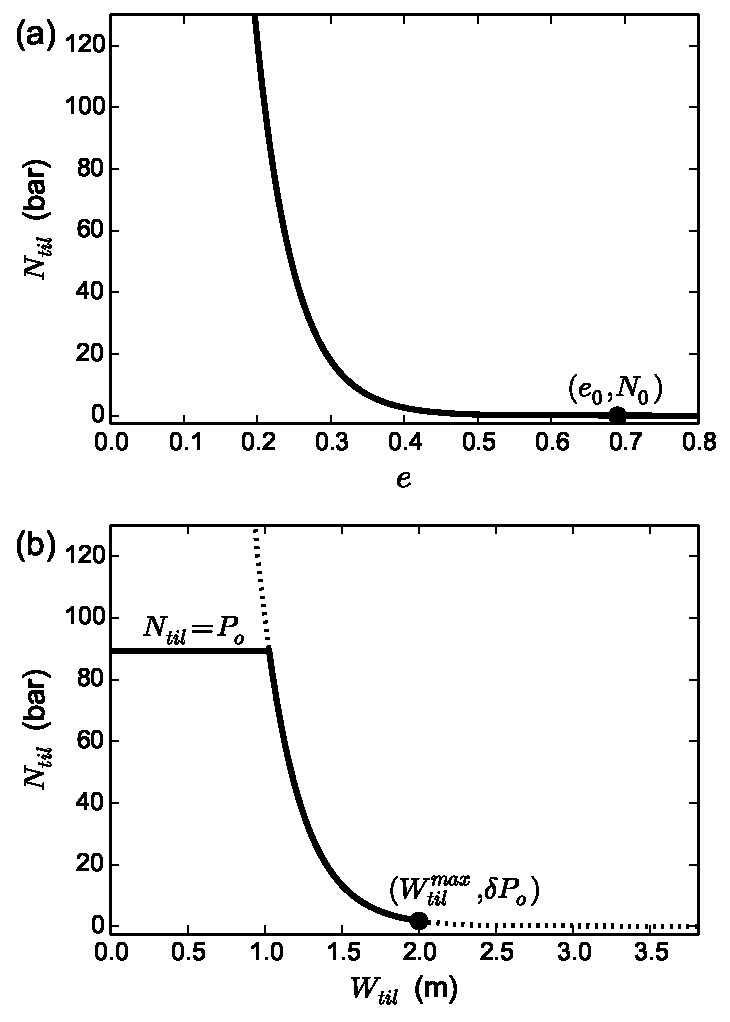
\includegraphics[width=3.0in,keepaspectratio=true]{Ntilfunctions}
\caption{\textbf{(a)} Equation \eqref{eq:voidpressure} determines the effective pressure $\Ntil$ as a function of the void ratio $e$\DIFdelbeginFL \DIFdelFL{, as shown here.  Reference }\DIFdelendFL \DIFaddbeginFL \DIFaddFL{; reference }\DIFaddendFL values \DIFdelbeginFL \DIFdelFL{of }\DIFdelendFL $e_0$\DIFdelbeginFL \DIFdelFL{and }\DIFdelendFL \DIFaddbeginFL \DIFaddFL{,}\DIFaddendFL $N_0$ are indicated.  \textbf{(b)}  The same curve, \DIFaddbeginFL \DIFaddFL{but }\DIFaddendFL with $\Ntil$ as a function of $\Wtil$, \DIFdelbeginFL \DIFdelFL{and  bounded }\DIFdelendFL \DIFaddbeginFL \DIFaddFL{with bounds }\DIFaddendFL above by overburden pressure $P_o$ and below by a fixed fraction $\delta$ of $P_o$\DIFdelbeginFL \DIFdelFL{(}\DIFdelendFL \DIFaddbeginFL \DIFaddFL{; the }\DIFaddendFL solid curve \DIFdelbeginFL \DIFdelFL{), }\DIFdelendFL is used in our model.  The case shown \DIFdelbeginFL \DIFdelFL{is for }\DIFdelendFL \DIFaddbeginFL \DIFaddFL{has }\DIFaddendFL 1000 meters ice thickness.}
\label{fig:Ntilfunctions}
\end{figure}

\begin{figure}[ht]
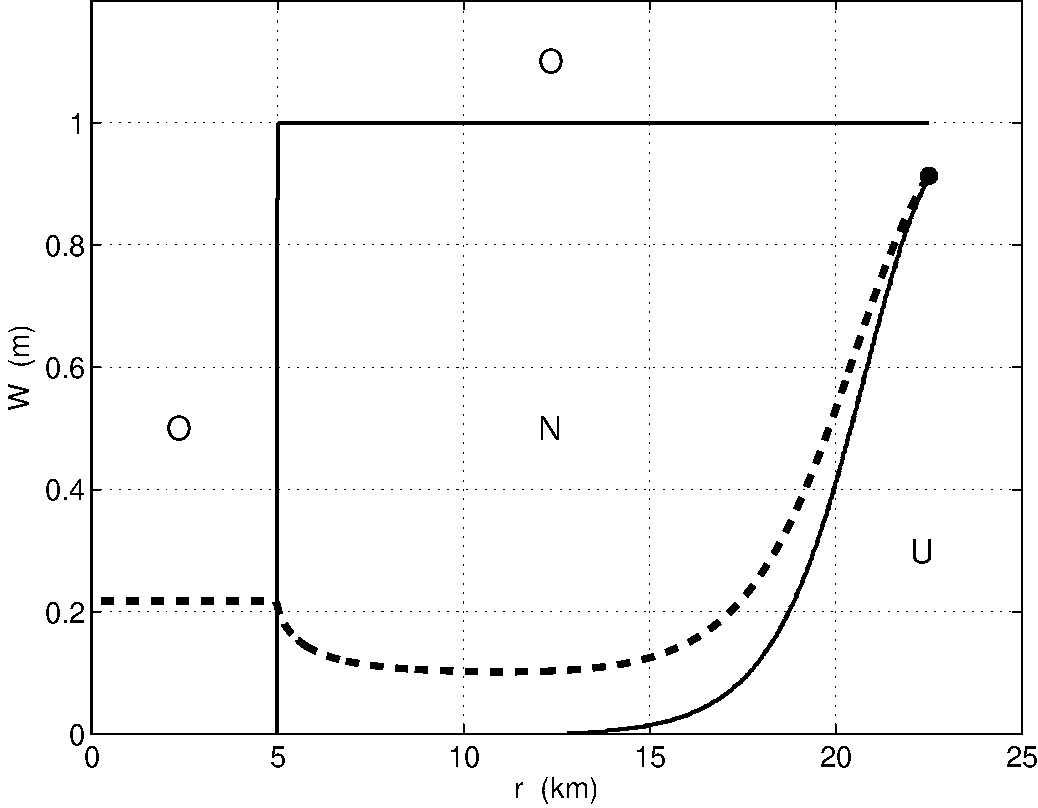
\includegraphics[width=3.0in,keepaspectratio=true]{exact-W-plot-onu}
\caption{\DIFdelbeginFL \DIFdelFL{An exact }\DIFdelendFL \DIFaddbeginFL \DIFaddFL{A nearly-exact }\DIFaddendFL radial, steady solution for water thickness $W(r)$ (dashed).  In $r$-versus-$W$ space the overpressure (O), normal pressure (N), and underpressure (U) regions \DIFaddbeginFL \DIFaddFL{(solid curves) }\DIFaddendFL are determined by ice geometry and sliding velocity\DIFdelbeginFL \DIFdelFL{(solid curves; see text)}\DIFdelendFL \DIFaddbeginFL \DIFaddFL{, because this is steady state}\DIFaddendFL .}
\label{fig:Wexact}
\end{figure}

\begin{figure}[ht]
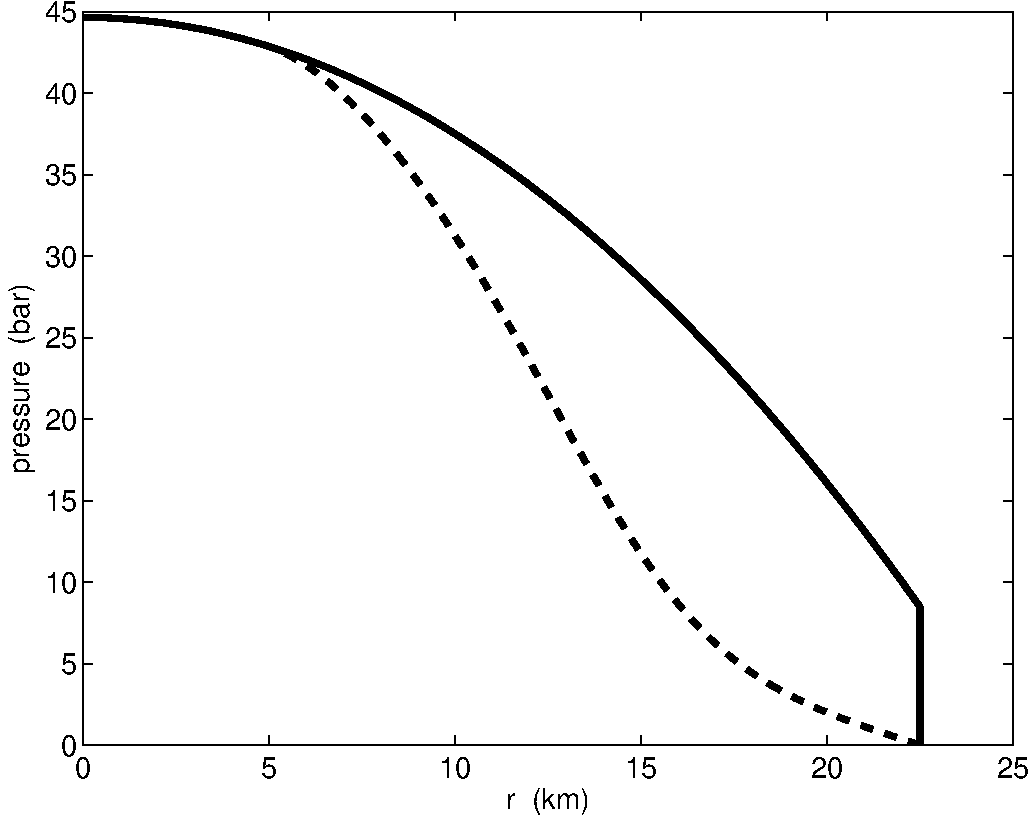
\includegraphics[width=3.0in,keepaspectratio=true]{exact-P-plot}
\caption{\DIFdelbeginFL \DIFdelFL{An exact }\DIFdelendFL \DIFaddbeginFL \DIFaddFL{A nearly-exact }\DIFaddendFL radial, steady solution \DIFaddbeginFL \DIFaddFL{for }\DIFaddendFL pressure $P(r)$ (dashed) and overburden pressure $P_o$ (solid).}
\label{fig:Pexact}
\end{figure}

\begin{figure}[ht]
\centering
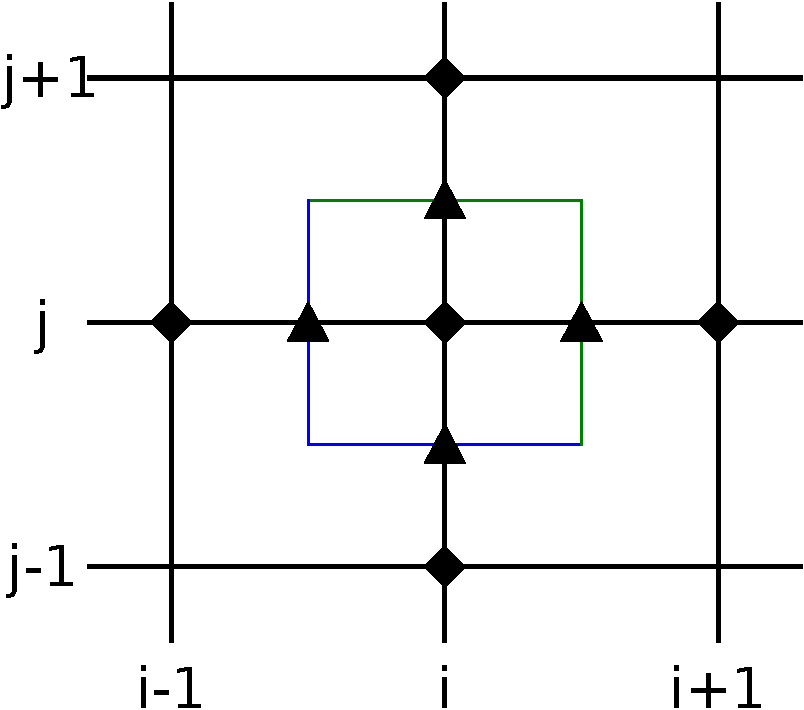
\includegraphics[width=2.2in,keepaspectratio=true]{diffstencil}
\bigskip
\caption{Numerical schemes \eqref{eq:Wfd} and \eqref{eq:Pfd} use a grid-point-centered cell.  Velocities, diffusivities, and fluxes are evaluated at staggered grid locations (triangles at centers of cell edges\DIFaddbeginFL \DIFaddFL{) }\DIFaddendFL denoted \DIFaddbeginFL \DIFaddFL{by compass notation }\DIFaddendFL $e,w,n,s$\DIFdelbeginFL \DIFdelFL{)}\DIFdelendFL .  State functions \DIFdelbeginFL \DIFdelFL{$W,P$ }\DIFdelendFL \DIFaddbeginFL \DIFaddFL{$W,W_{til},P$ }\DIFaddendFL are located at regular grid points (diamonds).}
\label{fig:stencil}
\end{figure}

\begin{figure}[ht]
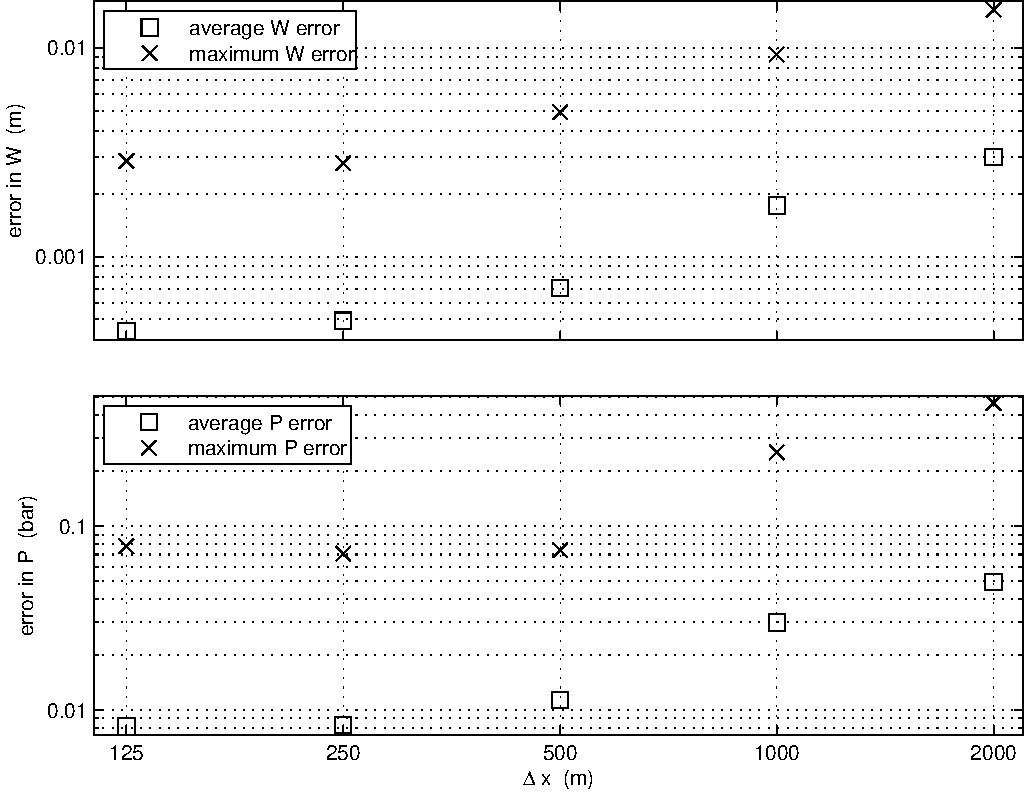
\includegraphics[width=3.0in,keepaspectratio=true]{refineWPpism}
\caption{Average water thickness error $|W-W_{exact}|$ decays as $O(\Delta x^{0.91})$, and average pressure error $|P-P_{exact}|$ decays as $O(\Delta x^{0.92})$, for grids with spacing $250 \le \Delta x = \Delta y \le 2000$ m.}
\label{fig:refineWPpism}
\end{figure}

\newcommand{\grnht}{3.4in}
\DIFdelbegin %DIFDELCMD < \begin{figure*}[ht]
%DIFDELCMD < %%%
%\DIFdel{\mbox{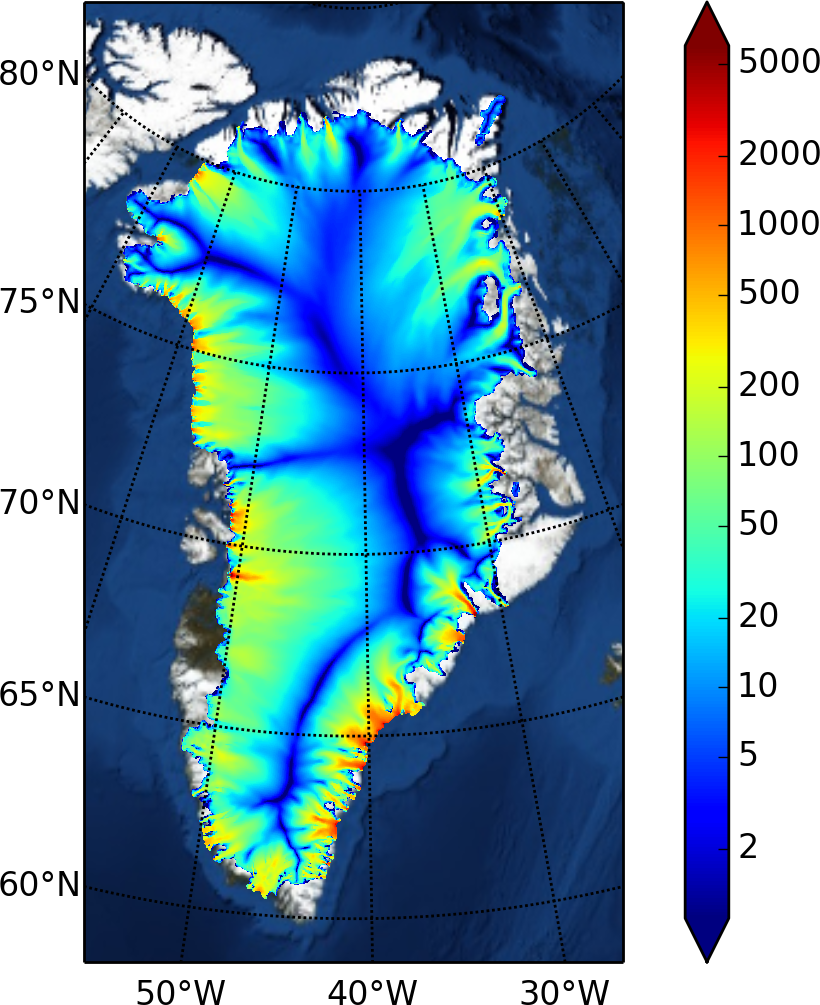
\includegraphics[height=\grnht,keepaspectratio=true]{g2km-init-velsurf-mag} \,
%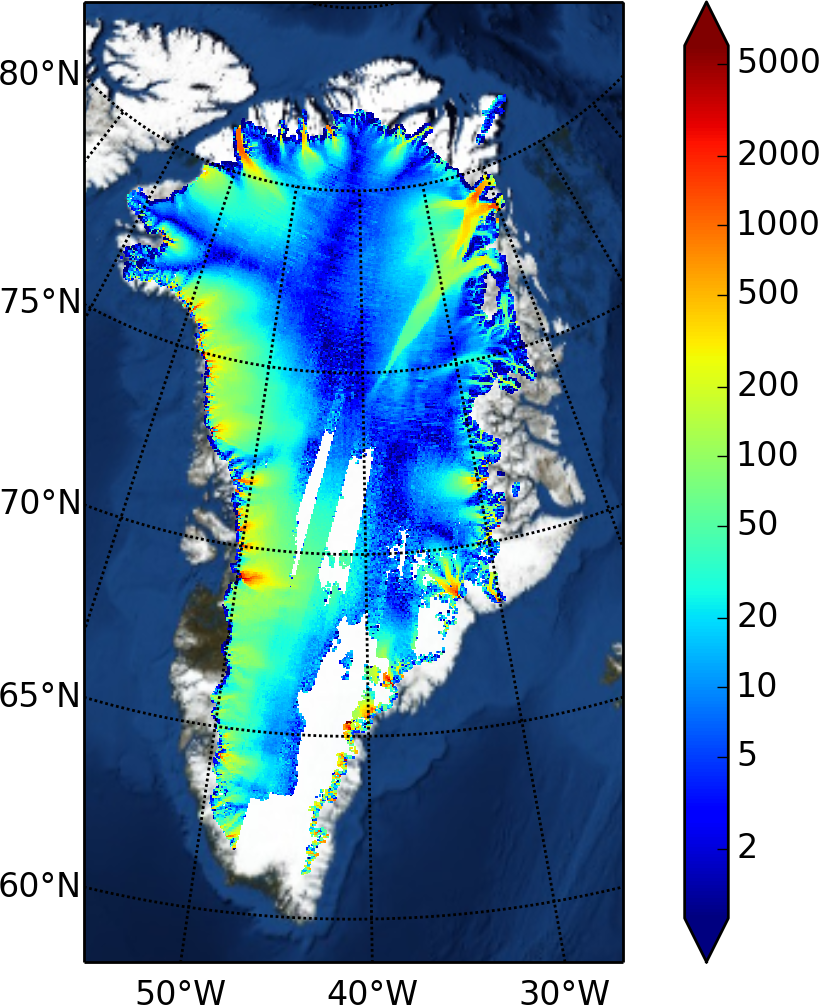
\includegraphics[height=\grnht,keepaspectratio=true]{Greenland-surfvelmag}}
%}%DIFDELCMD < \caption{%
{%DIFAUXCMD
\DIFdel{To evaluate the result of the 2 km grid spun-up ice dynamical model we compare modelled ice speed at the ice surface (left; $\mathrm{m}\,\mathrm{a}^{-1}$) to satellite observations (right; $\mathrm{m}\,\mathrm{a}^{-1}$).}}
%DIFAUXCMD
%DIFDELCMD < \label{fig:Greenspinupeval}
%DIFDELCMD < \end{figure*}
%DIFDELCMD < %%%
\DIFdelend 

\begin{figure*}[ht]
\mbox{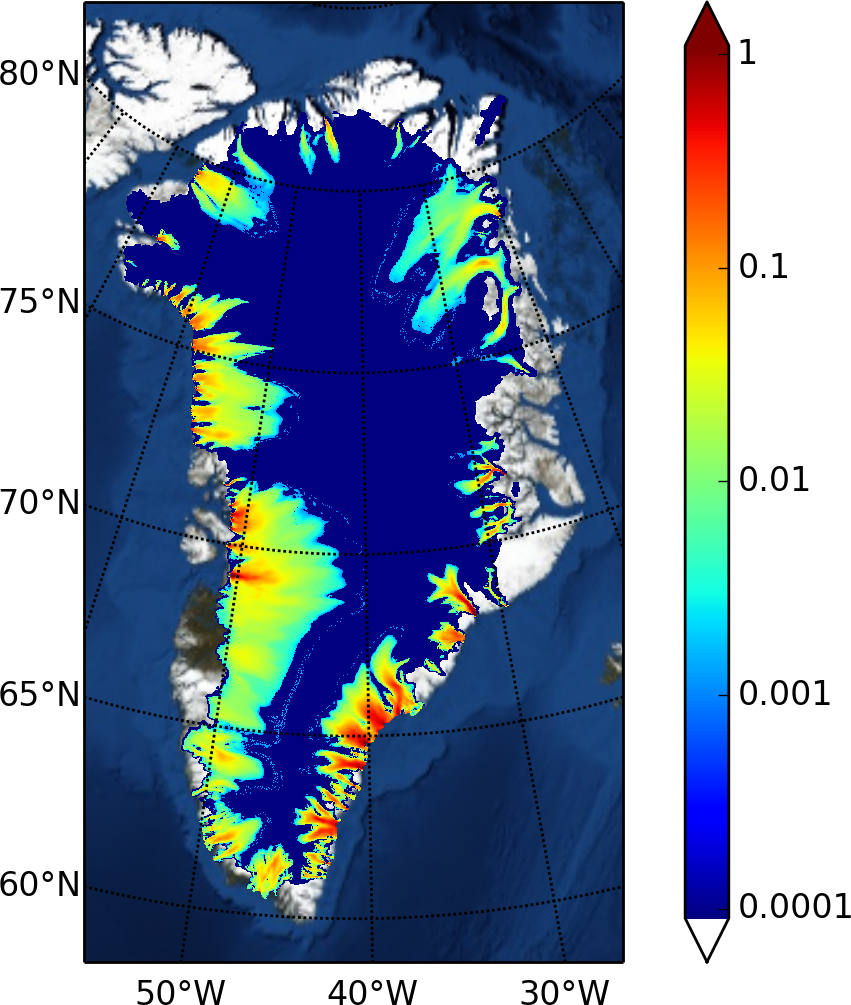
\includegraphics[height=\grnht,keepaspectratio=true]{g2km-init-bmelt} \,
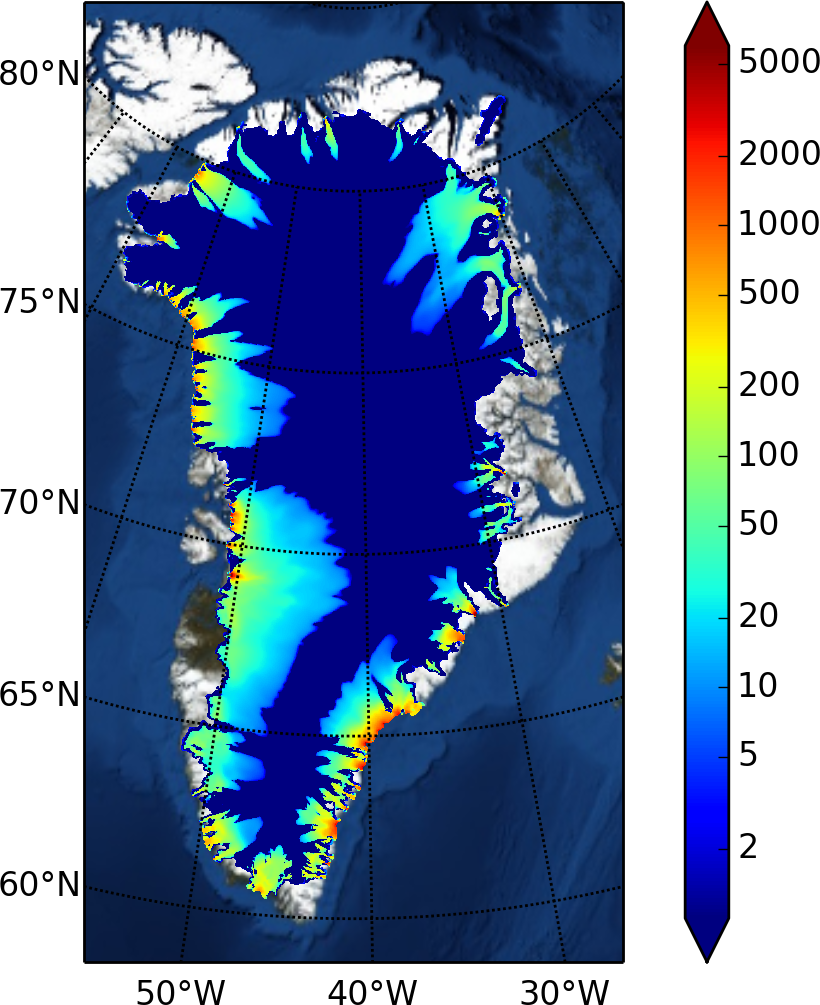
\includegraphics[height=\grnht,keepaspectratio=true]{g2km-init-velbase-mag}}
\caption{The inputs to the hydrology model are the modeled basal melt rate $m/\rho_w$ (left; $\mathrm{m}\,\mathrm{a}^{-1}$) and sliding speed $|\bv_b|$ (right; $\mathrm{m}\,\mathrm{a}^{-1}$) from the spun-up \DIFdelbeginFL \DIFdelFL{model}\DIFdelendFL \DIFaddbeginFL \DIFaddFL{state}\DIFaddendFL .}
\label{fig:Greenhydroinputs}
\end{figure*}

\begin{figure*}[ht]
\mbox{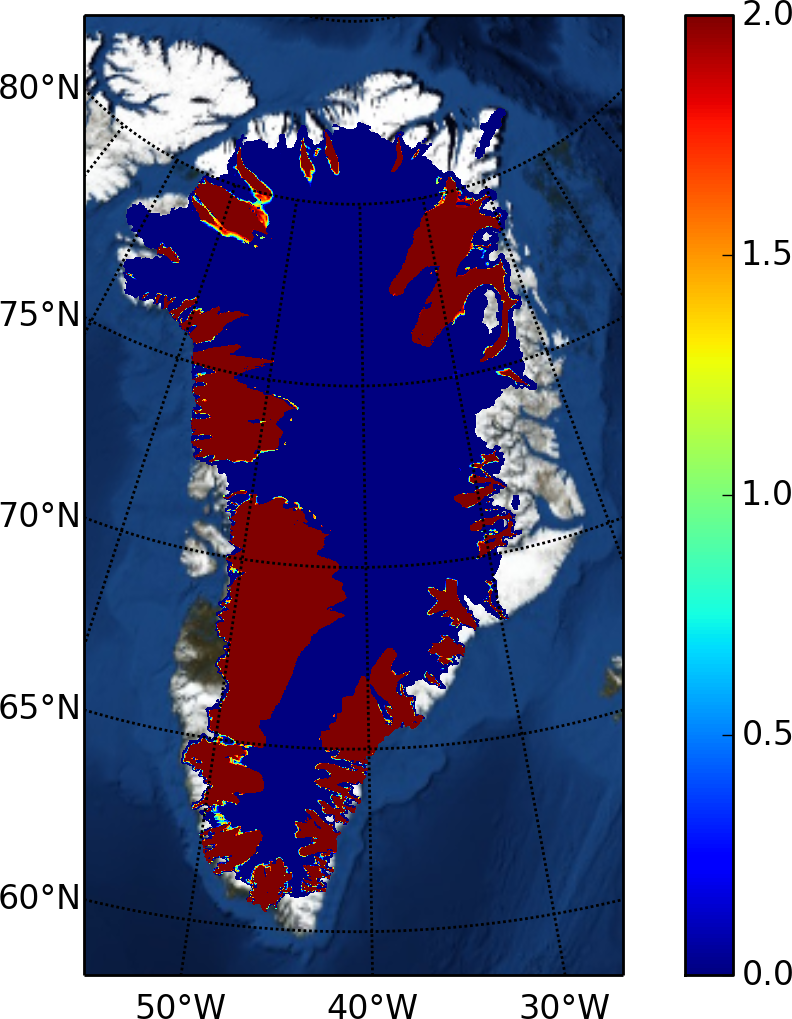
\includegraphics[height=\grnht,keepaspectratio=true]{routing-decoupled-tillwat} \,
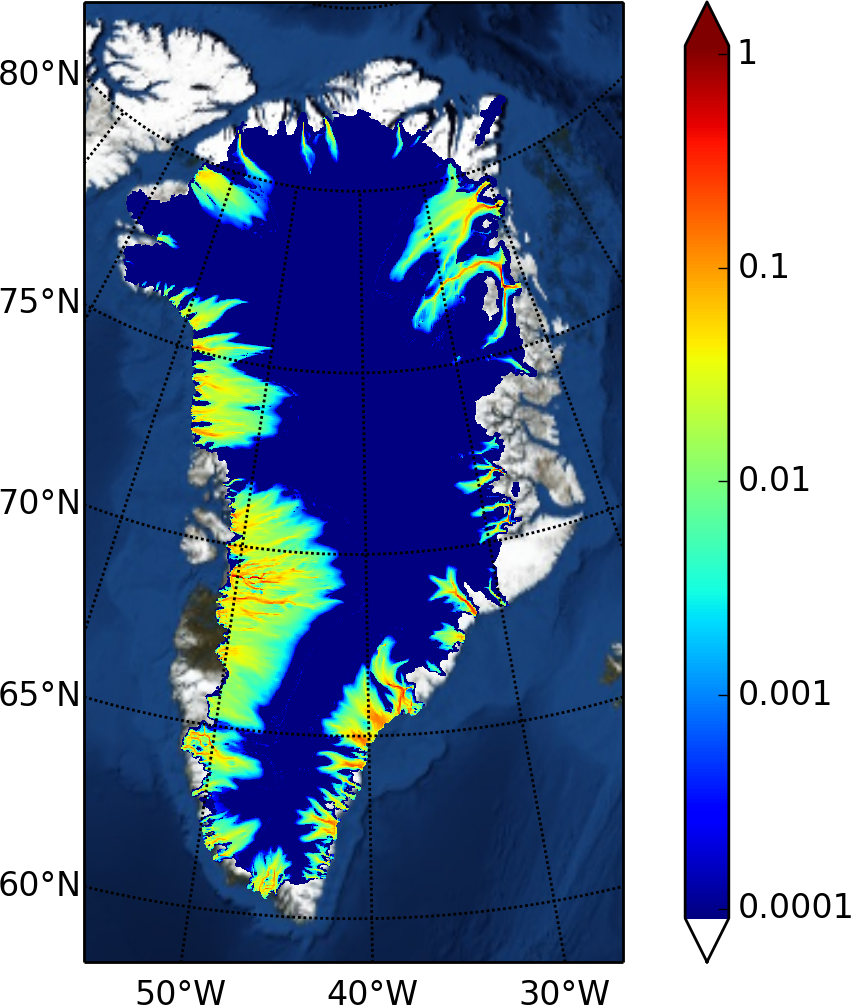
\includegraphics[height=\grnht,keepaspectratio=true]{routing-decoupled-bwat}}
\caption{Outputs from the \texttt{routing} hydrology model are the modelled till-stored water layer thickness $\Wtil$ (left; $\mathrm{m}$) and modelled transportable water layer thickness $W$ (right; $\mathrm{m}$).}
\label{fig:Greenroutingresults}
\end{figure*}

\begin{figure*}[ht]
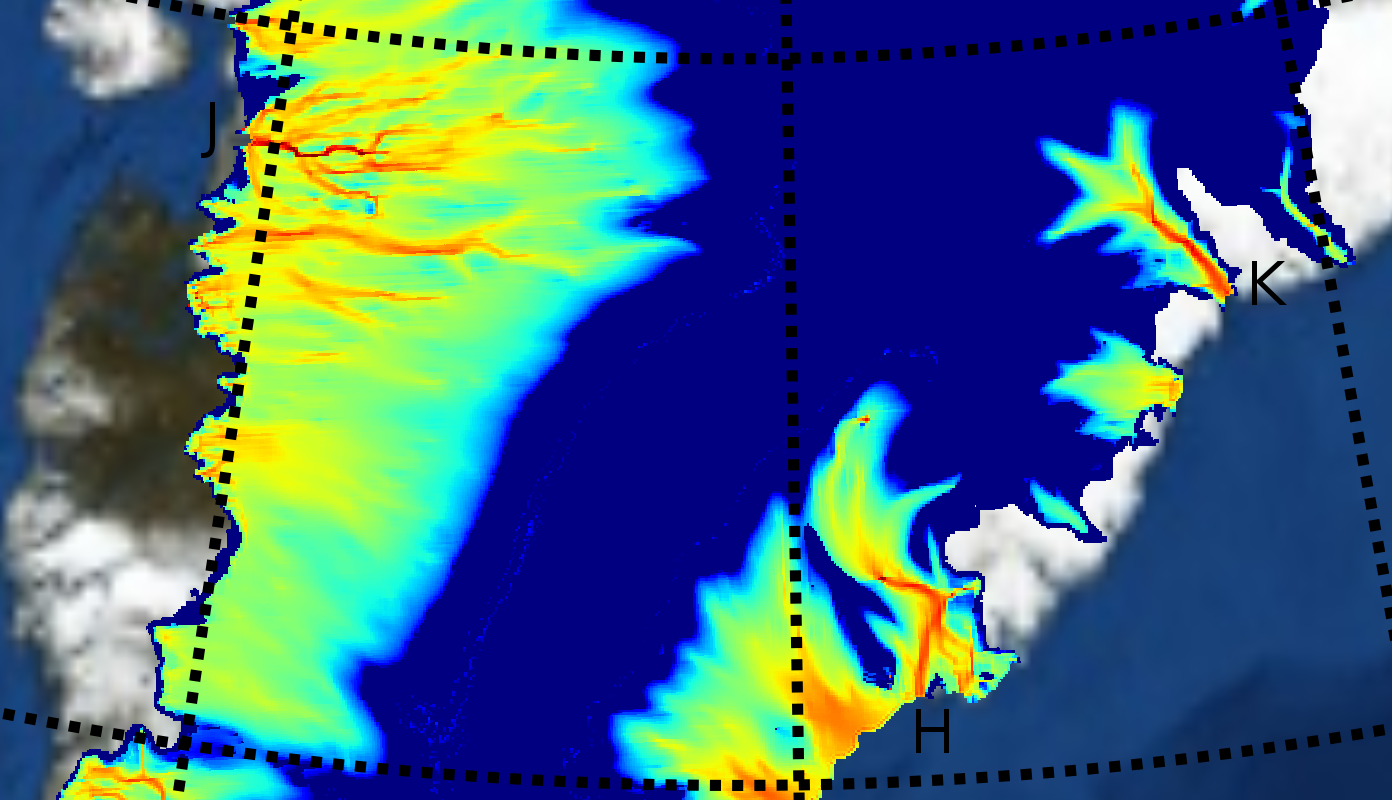
\includegraphics[height=2.7in,keepaspectratio=true]{detail-routing-decoupled-bwat}
\caption{Detail of transportable water $W$ plotted in Figure \ref{fig:Greenroutingresults}, covering Jakobshavn (J), Helheim (H), and Kangerdlugssuaq (K) outlet glaciers}
\label{fig:Greenroutingdetail}
\end{figure*}

\begin{figure*}[ht]
\mbox{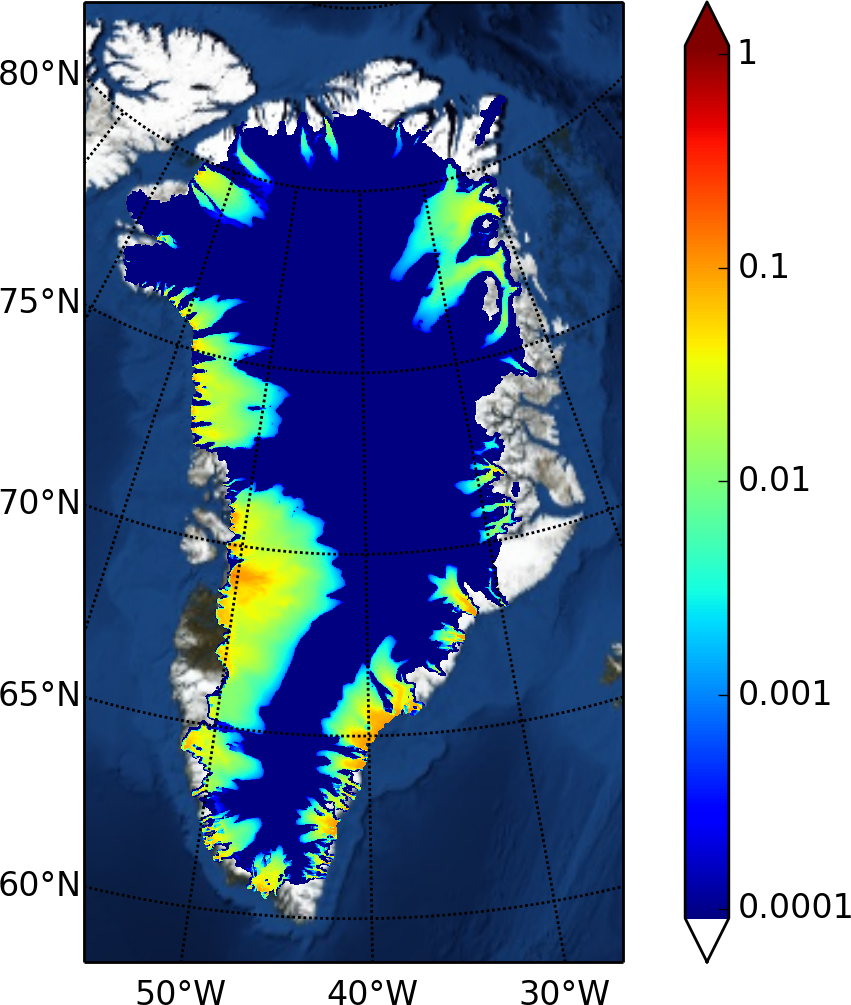
\includegraphics[height=\grnht,keepaspectratio=true]{distributed-decoupled-bwat} \,
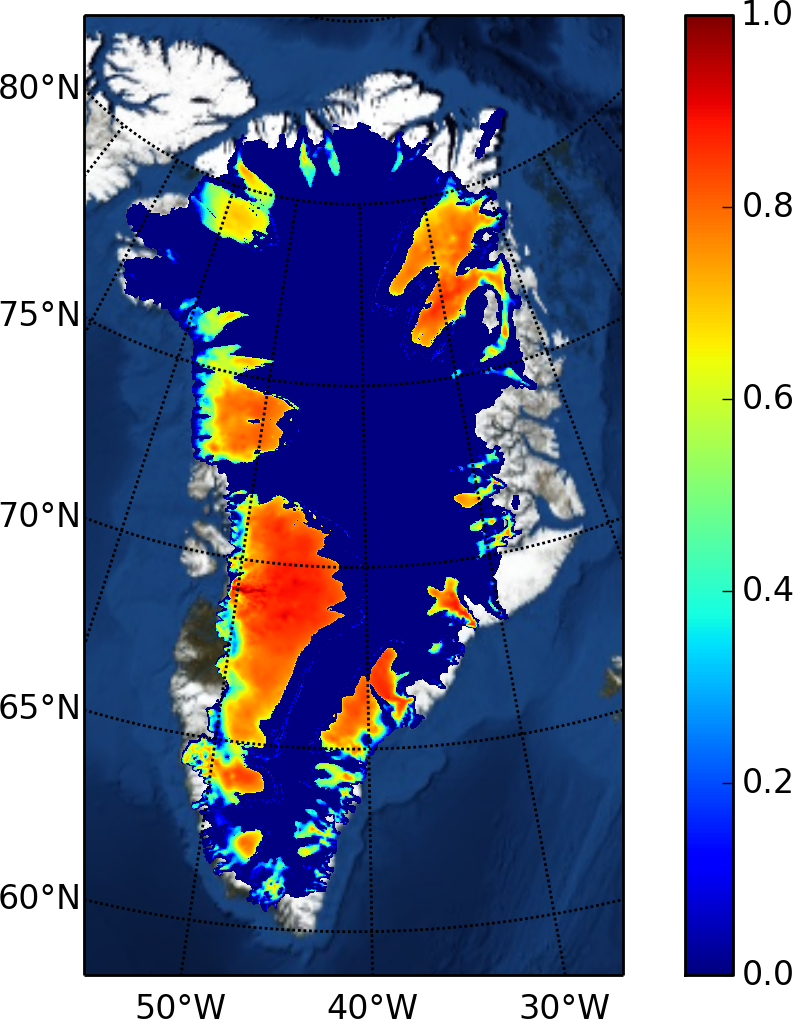
\includegraphics[height=\grnht,keepaspectratio=true]{distributed-decoupled-bwprel}}
\caption{Outputs from the \texttt{distributed} hydrology model include the modelled transportable water layer thickness $W$ (left; $\mathrm{m}$), and the modelled transportable water layer pressure \DIFaddbeginFL \DIFaddFL{$P$}\DIFaddendFL , shown relative to overburden pressure \DIFdelbeginFL \DIFdelFL{$P/P_o$ }\DIFdelendFL (\DIFaddbeginFL \DIFaddFL{i.e.~$P/P_o$; }\DIFaddendFL right).}
\label{fig:Greendistributedresults}
\end{figure*}

\newcommand{\myheight}{1.8in}
\begin{figure*}[ht]
\mbox{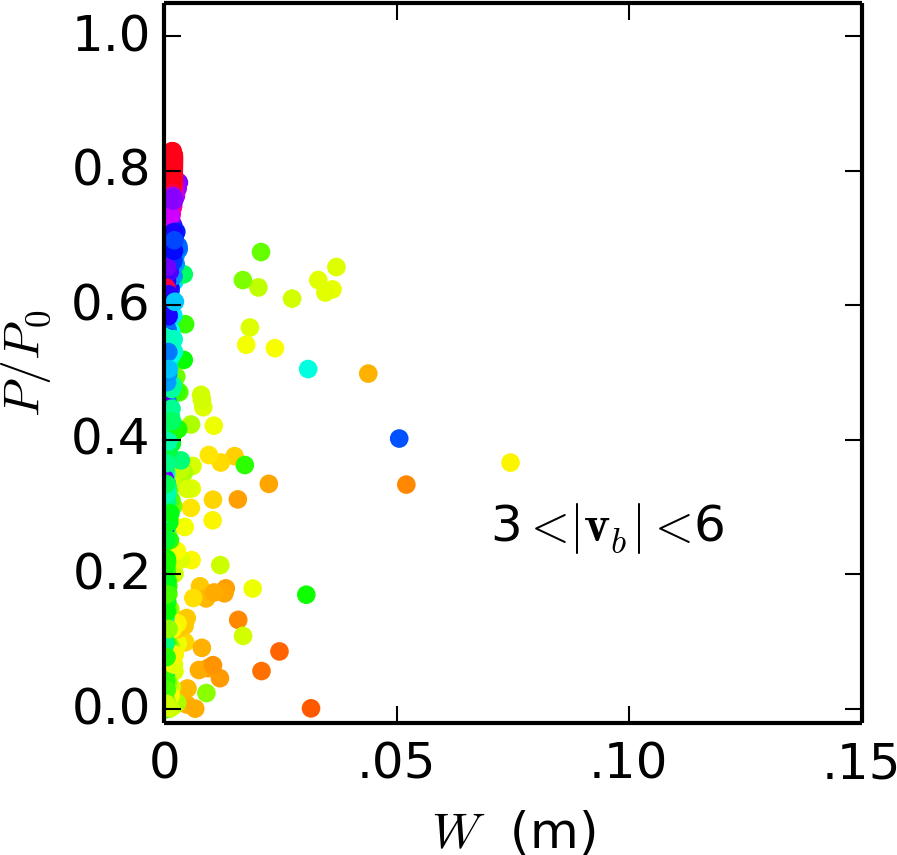
\includegraphics[height=\myheight,keepaspectratio=true]{bin1-g2km} \, 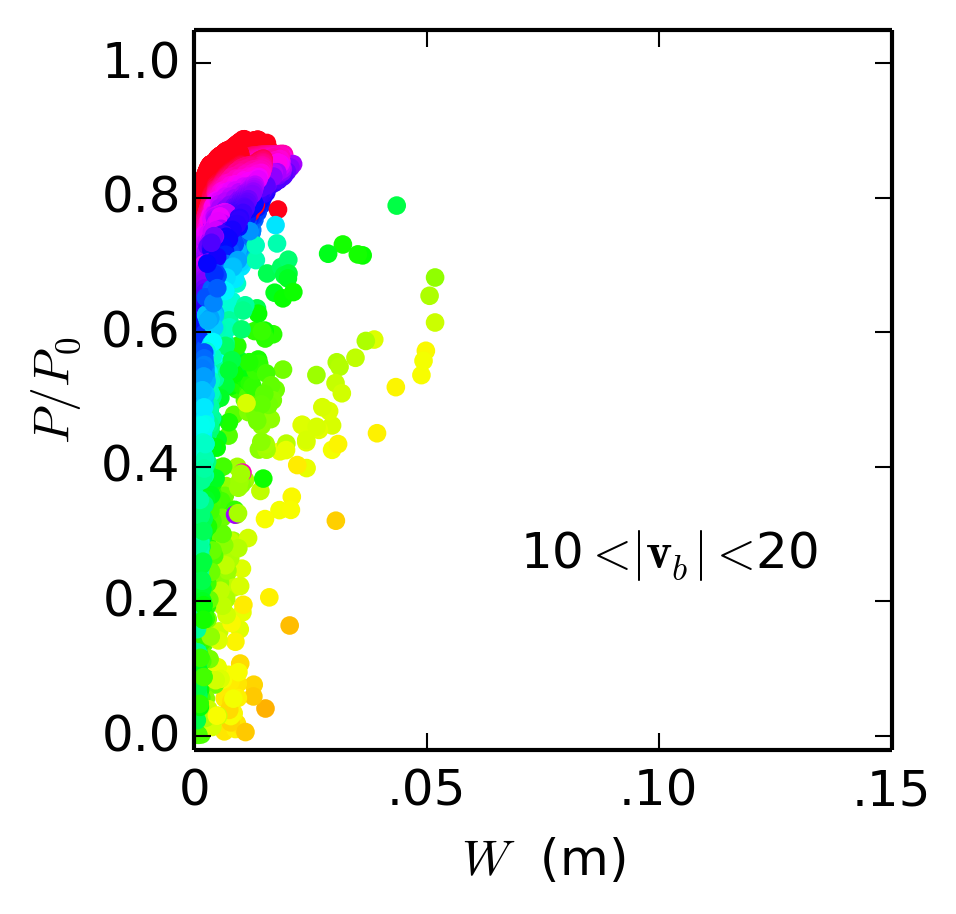
\includegraphics[height=\myheight,keepaspectratio=true]{bin10-g2km} \, 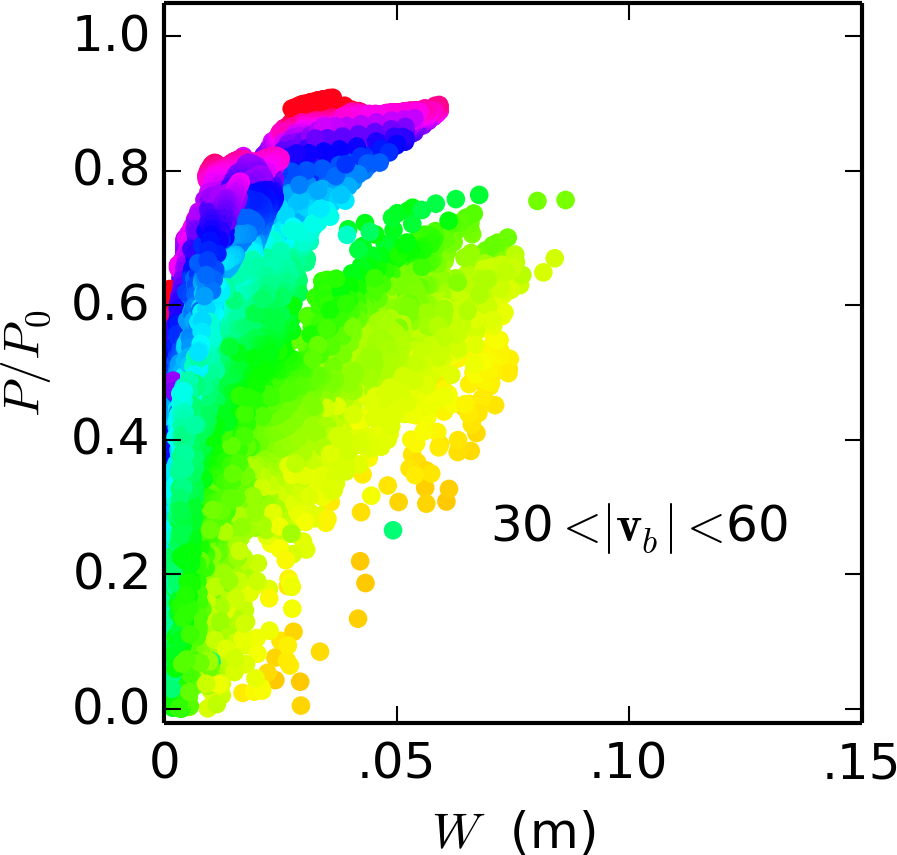
\includegraphics[height=\myheight,keepaspectratio=true]{bin30-g2km}}
\mbox{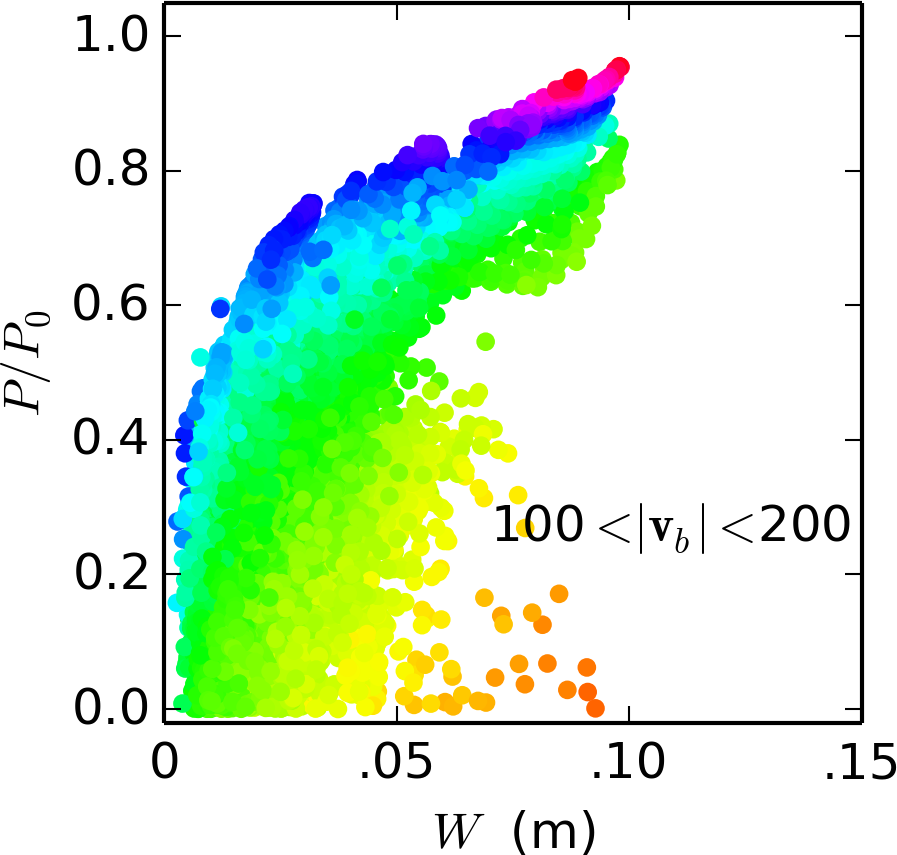
\includegraphics[height=\myheight,keepaspectratio=true]{bin100-g2km} \,
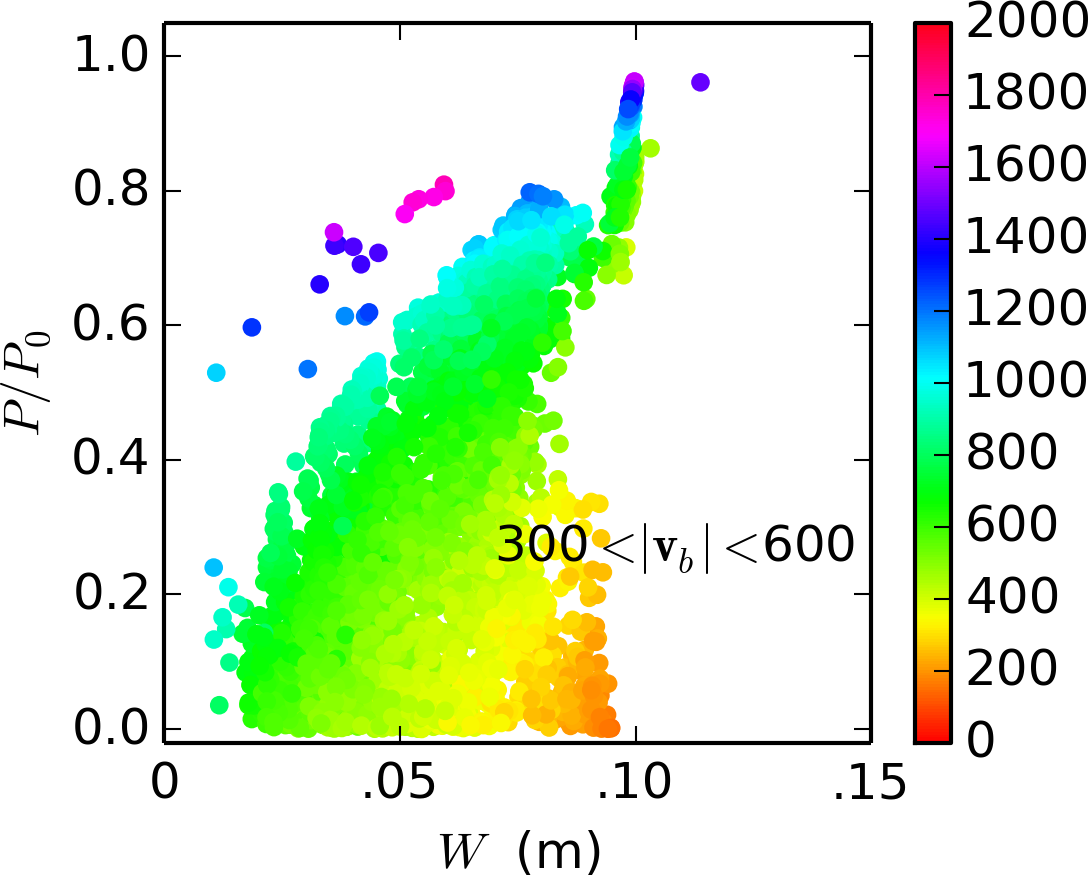
\includegraphics[height=1.85in,keepaspectratio=true]{bin300-g2km}}
\caption{Scatter plots of \DIFdelbeginFL \DIFdelFL{$(W,P)$ }\DIFdelendFL \DIFaddbeginFL \DIFaddFL{$(W,P/P_o)$ }\DIFaddendFL pairs for all cells \DIFdelbeginFL \DIFdelFL{at end of a 5 model year steady-input simulation on a 2 km grid for }\DIFdelendFL \DIFaddbeginFL \DIFaddFL{from }\DIFaddendFL the \DIFdelbeginFL \DIFdelFL{whole Greenland ice sheet using }\DIFdelendFL \DIFaddbeginFL \texttt{\DIFaddFL{distributed}} \DIFaddFL{model run, which used }\DIFaddendFL roughness scale $W_r = 0.1$ m.  Each \DIFdelbeginFL \DIFdelFL{scatter plot }\DIFdelendFL \DIFaddbeginFL \DIFaddFL{sub-plot only }\DIFaddendFL shows \DIFdelbeginFL \DIFdelFL{the }\DIFdelendFL pairs \DIFdelbeginFL \DIFdelFL{for a select }\DIFdelendFL \DIFaddbeginFL \DIFaddFL{from the indicated }\DIFaddendFL range of ice sliding speeds\DIFdelbeginFL \DIFdelFL{, as indicated}\DIFdelendFL .  Points are colored by ice thickness using a common scale shown beside last figure.}
\label{fig:GreenisPofW}
\end{figure*}

\begin{figure}[ht]
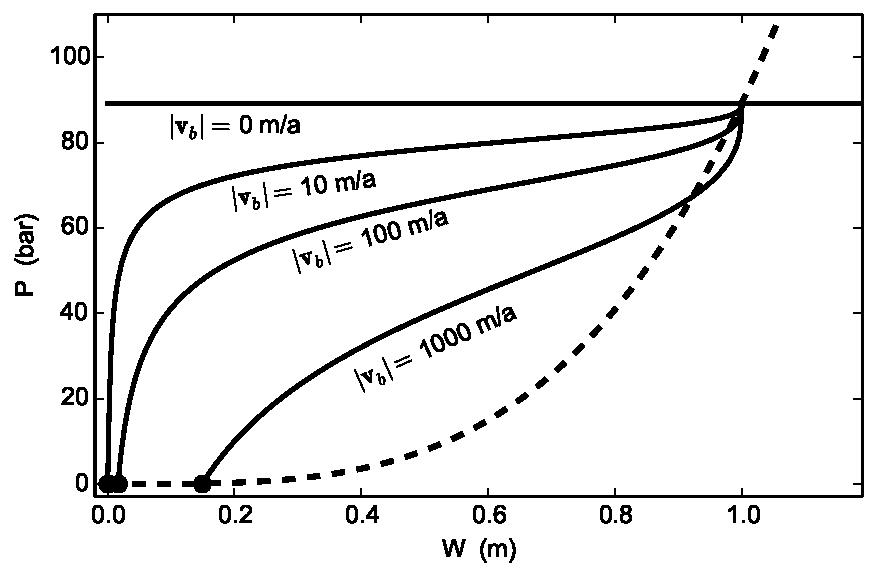
\includegraphics[width=2.8in,keepaspectratio=true]{psteady-vb}
\caption{The steady state function $P(W)$ defined by equation \eqref{eq:PofWsteady}\DIFdelbeginFL \DIFdelFL{depends on the sliding speed $|\bv_b|$.  Four cases are shown.  All use }\DIFdelendFL \DIFaddbeginFL \DIFaddFL{, using }\DIFaddendFL $W_r=1$ m and \DIFdelbeginFL \DIFdelFL{a uniform ice thickness of }\DIFdelendFL $H=1000$ m \DIFaddbeginFL \DIFaddFL{(solid curves)}\DIFaddendFL .  Values of $W_c$ are indicated by black dots at $P=0$.  \DIFdelbeginFL \DIFdelFL{Relation }\DIFdelendFL \DIFaddbeginFL \DIFaddFL{For comparison, \mbox{%DIFAUXCMD
\cite{FlowersClarke2002_theory}
}%DIFAUXCMD
relation }\DIFaddendFL \eqref{eq:PofWFC} \DIFdelbeginFL \DIFdelFL{(dashed black) }\DIFdelendFL is shown with $W_{\text{crit}}=1$ m \DIFdelbeginFL \DIFdelFL{for comparison}\DIFdelendFL \DIFaddbeginFL \DIFaddFL{(dashed black)}\DIFaddendFL .}
\label{fig:psteady-vb}
\end{figure}

\begin{figure}[ht]
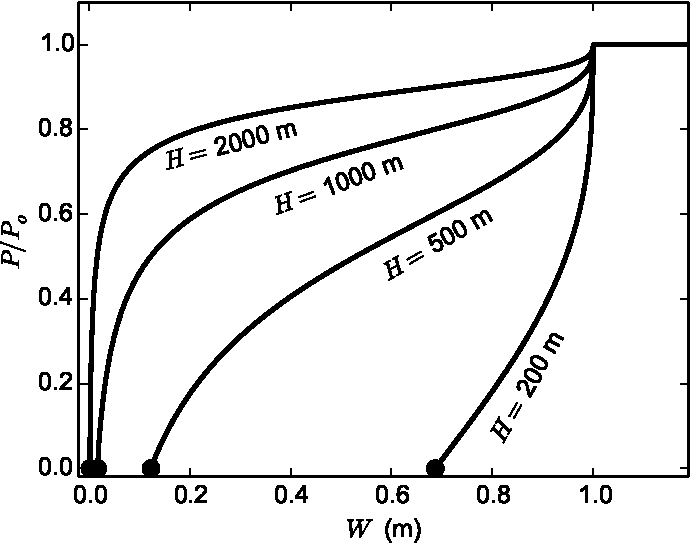
\includegraphics[width=2.8in,keepaspectratio=true]{psteady-Po}
\caption{The graph of $P(W)$ defined by \eqref{eq:PofWsteady} also depends on overburden pressure $P_o=\rho_i g H$\DIFdelbeginFL \DIFdelFL{.  We fix }\DIFdelendFL \DIFaddbeginFL \DIFaddFL{, shown using }\DIFaddendFL $|\bv_b|=100$ m/a and $W_r=1$ m\DIFdelbeginFL \DIFdelFL{and consider four cases of uniform thickness $H$}\DIFdelendFL .}
\label{fig:psteady-Po}
\end{figure}

\end{document}
